%This is my masters project report
\documentclass[a4paper,twoside]{report}
\usepackage{etoolbox}
\usepackage[utf8]{inputenc}
\usepackage{wrapfig}
\usepackage{subcaption}
\usepackage{amsmath}
\usepackage{url}
\usepackage{graphicx}
\usepackage{lipsum}
\usepackage{fancyhdr}
\usepackage{listings}
\usepackage{lastpage}
\usepackage[margin=0.8in]{geometry}
\usepackage[resetfonts]{cmap}
\usepackage{fancyvrb}
\begin{VerbatimOut}{ot1.cmap}
/CIDInit /ProcSet findresource begin
12 dict begin
begincmap
/CIDSystemInfo
<< /Registry (TeX)
/Ordering (OT1)
/Supplement 0kws 2018
>> def
/CMapName /TeX-OT1-0 def
/CMapType 2 def
1 begincodespacerange
<00> <7F>
endcodespacerange
8 beginbfrange
<00> <01> <0000>
<09> <0A> <0000>
<23> <26> <0000>
<28> <3B> <0000>
<3F> <5B> <0000>
<5D> <5E> <0000>
<61> <7A> <0000>
<7B> <7C> <0000>
endbfrange
40 beginbfchar
<02> <0000>
<03> <0000>
<04> <0000>
<05> <0000>
<06> <0000>
<07> <0000>
<08> <0000>
<0B> <0000>
<0C> <0000>
<0D> <0000>
<0E> <0000>
<0F> <0000>
<10> <0000>
<11> <0000>
<12> <0000>
<13> <0000>
<14> <0000>
<15> <0000>
<16> <0000>
<17> <0000>
<18> <0000>
<19> <0000>
<1A> <0000>
<1B> <0000>
<1C> <0000>
<1D> <0000>
<1E> <0000>
<1F> <0000>
<21> <0000>
<22> <0000>
<27> <0000>
<3C> <0000>
<3D> <0000>
<3E> <0000>
<5C> <0000>
<5F> <0000>
<60> <0000>
<7D> <0000>
<7E> <0000>
<7F> <0000>
endbfchar
endcmap
CMapName currentdict /CMap defineresource pop
end
end
\end{VerbatimOut}
\numberwithin{equation}{section}
\pagestyle{fancy}
\fancyhf{}
\rhead{Ankush B}
\lhead{Project Report for MSc 2 - ASTROSAT}
\cfoot{\thepage-\pageref{LastPage}}
\newcommand\eqline[1]{\begin{equation} #1 \end{equation}}
\newcommand\hfrac{\frac{\hbar^2}{2m}}
\newcommand\dif[2]{\frac{d #1}{d #2}}
\newcommand\diff[2]{\frac{d^2 #1}{d #2^2}}
\newcommand\oneby[1]{\frac{1}{#1}}
\newcommand\pdif[2]{ \frac{\partial #1}{\partial #2}}
\newcommand\sun{\cdot}
\newcommand{\pth}{$^{th}$}
\title{The Spectral and Temporal study of Neutron Star Ultra Comapct X-ray Binary 1A 1246-588}
\author{Ankush Banerjee}
\begin{document}
\maketitle
\begin{abstract}
Ultra Compact X-ray Binaries are a rare and mysterious class of Low Mass X-ray Binaries that have a companion with an orbital period less than an hour. These could be differentiated by the primary star being either a Neutron Star or a Black Hole. In the case of 1A 1246-588, the primary star is known to be a Neutron star, with a white dwarf companion, however, it’s orbital period is a mystery, given it’s low X-ray luminosity. Since there are no direct observation of it’s orbital period, the following work is to first, familiarize myself with the tools of the trade, the things that I would be using to analyze astrophysical data, and then try to probe the temporal and spectral properties of 1A 1246-588 using SXT and LAXPC data. Given the data, what I found has remained largely inconclusive as of now, however, comparison of the above with other satellite data remains to be done. The main intention of the project was for me to familiarize myself with the data analysis techniques used in astrophysical research and do some data analysis along the way so as to help me understand, to a certain degree how X-ray data is to be analyzed.
\end{abstract}
\newpage
\tableofcontents{}
\newpage
\chapter{Acknowledgement}
\paragraph{}
First of all I would like to thank my parents for being the unshakable pillars of my life, I fail to imagine a life without their support, whatever I am is because of them both literally and figuratively. I would also like to thank my guide Dr. Sudip Bhattacharya (TIFR) who took me in as his mentee and bestowed upon me the much needed guidance and resources for this project. His role has been paramount in developing my understanding of high energy astrophysics and I can see it become my love already. Apart from giving me access to the much needed data he allowed me to sit in for the astronomy course given at TIFR by him, which I should say was one of the best experiences I've had till date. I would also like to thank Mr. Vikas Chand (TIFR) for helping me understand the nuances of spectral analysis and for sharing how it is supposed to be done. I would also like to thank my firends who have put up with my tantrums and mood swings during my college days and never gave up on me, I would've never completed my work if it were not for them. I would also like to thank my professors at K. J. Somaiya College of Science and Commerce for allowing me to take a project outside my college, and guiding me through the official technicalities of the same. 
\newpage
\chapter{Introduction to ASTROSAT}
\paragraph{}
Analyzing and understanding the data one receives from X-ray satellites is something that is paramount in understanding high energy events transpiring within the cosmos. Most of the events that lead to the release of x-rays are generally very high energy events. Such extreme environments are the only regions in space where one can test the limits of physics, which, in some cases are near impossible to recreate (yet) in a “controlled” environment, not to mention the hazards associated with such experiments. This leads us to the frontiers of physics, after which everything is unknown, and exciting.
\paragraph{}
\begin{figure}[h]
\begin{subfigure}{0.4\textwidth}
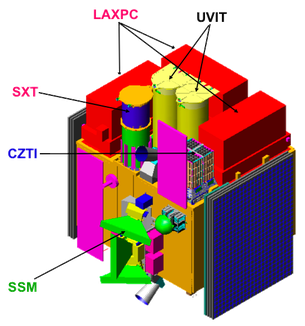
\includegraphics[width=1.0\linewidth]{Astrosat_folded_large.png} 
\caption{Astrosat With Payloads}
\label{Astrosat With Payload}
\end{subfigure}
\begin{subfigure}{0.6\textwidth}
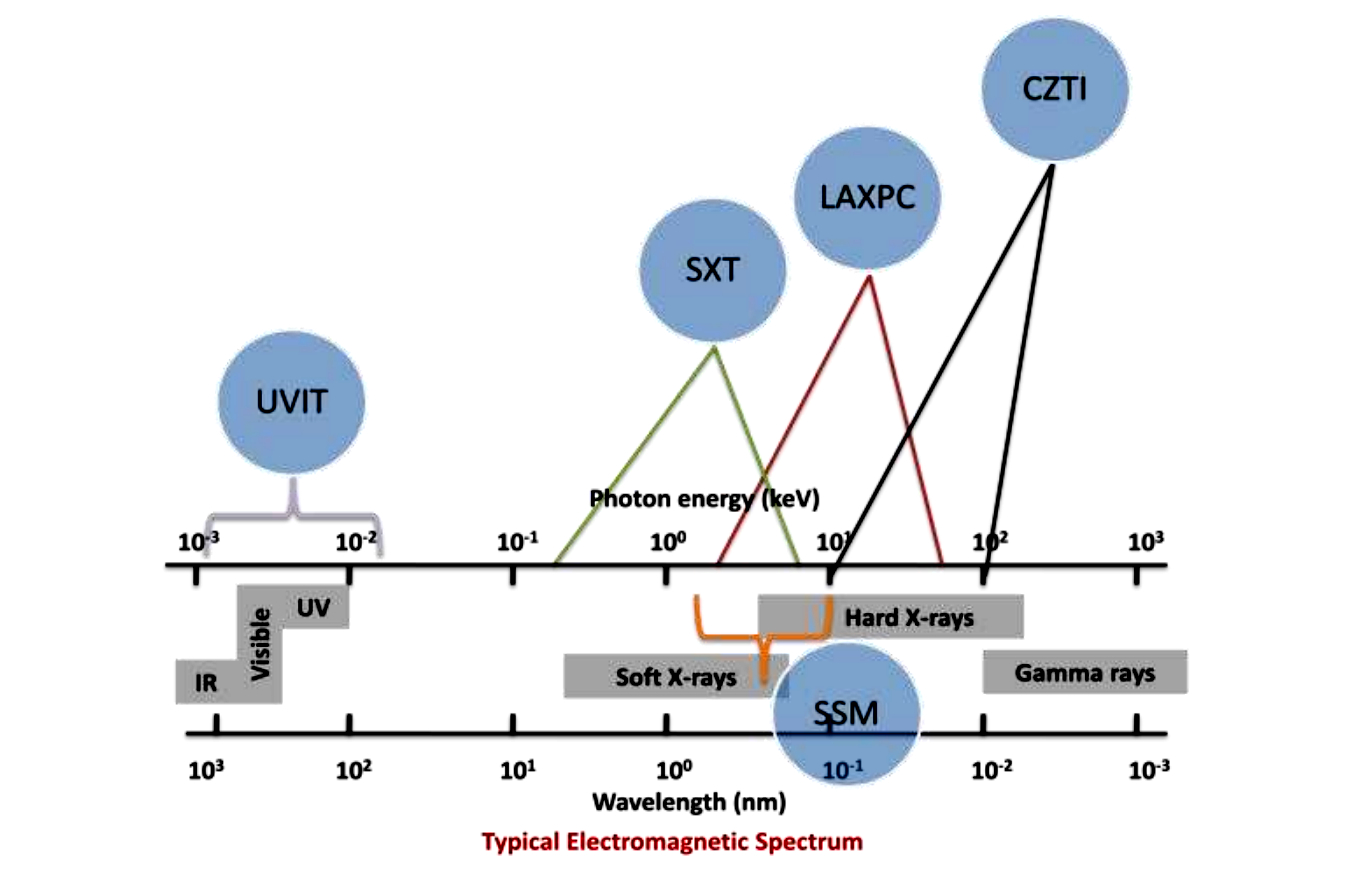
\includegraphics[width=1.0\linewidth, height=6cm]{Im2.jpg}
\caption{Wavelength Sensitivity of the Instruments}
\label{Wavelength Sensitivity}
\end{subfigure}
\caption{The Astrosat with its payloads and their wavelength sensitivities}
\label{fig:Wavelength Sensitivity}
\end{figure}
ASTROSAT is India's first multi-wavelength satellite dedicated to science, and aboard it are several instruments that look at different wavebands of the electromagnetic spectrum. They are:
\begin{description}
  \item[$\bullet$ Instrument 1] Soft X-ray Telescope (SXT)
  \item[$\bullet$ Instrument 2] Large Area X-ray Proportional Counter (LAXPC)
  \item[$\bullet$ Instrument 3] Ultra-Violet Imaging Telescope (UVIT)
  \item[$\bullet$ Instrument 4] Cadmium Zinc Telluride Imager (CZTI)
  \item[$\bullet$ Instrument 5] Scanning Sky Monitor (SSM)
\end{description}
\paragraph{}
Since the intensity of any source is a time dependent variable, simultaneous observations of such a source is very important to be able to derive much more information from a single event in various wavebands giving us a broad understanding of an event. Hence the availability of such an instrument saves the logistical difficulties one might face while gathering the same time interval data from different satellites/observatories. 
\paragraph{}
Out of the five primary payloads aboard the satellite, my work focused on the first two payloads mentioned. Namely, SXT and LAXPC since they are the ones that are sensitive to the the soft ($~0.3$ to $8$ $KeV$) and hard (above $8$ $KeV$) x-rays.
\section{Introduction to the Soft X-ray Telescope}
\paragraph{}
SXT, as the name suggests is sensitive to soft X-rays, that is, photons between the energy range $0.3$-$8.0$ $KeV$. Wavelengths of this energy range are responsive to focusing and hence will have a higher angular resolution, allowing it to discern between different sources very close to each other. To be more precise, it will be able to resolve between two x ray sources separated by an arc min. It will be able to perform Spatially Resolved Spectroscopy, and perform several variability studies on its sources.
\subsection{Focusing The X-Rays}
\paragraph{}
\begin{wrapfigure}{l}{0.5\textwidth}
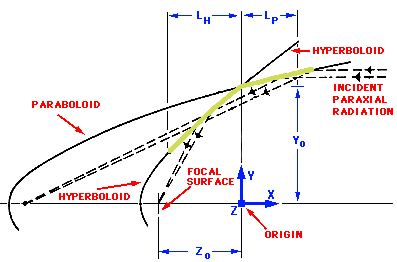
\includegraphics[width=0.9\linewidth]{paraboloid_hyperboloid.png} 
\caption{Wolter-$1$ Optics}
\label{fig:Wolter-1 optics}
\end{wrapfigure} 
The telescope consists of tubular gold foils which act as X-ray reflecting mirrors by employing the grazing incidence technique. Since the Refractive Index (R.I). of a metal, for X rays is slightly lesser than one, it is possible to get a total external reflection at a vacuum metal interface. The limiting angle for grazing incidence is a few degrees at $0.1$ $KeV$ and a few arc minutes at $10$ $KeV$. Sections of the paraboloid surfaces can be made to focus X rays via grazing incidences. However, this arrangement violates the Abbe sine Condition and hence the images in the focal plane seriously suffer from coma. However, this can be avoided by using a second hyperboloidal surface. This arrangement is called the Wolter-$1$ optical arrangement and has been adopted in most of the optical telescopes flown till today. 
\paragraph{}
\begin{wrapfigure}{r}{0.5\textwidth}
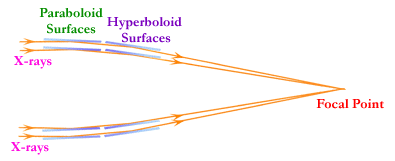
\includegraphics[width=1.0\linewidth]{teles2_th.png} 
\caption{Mirror Nesting}
\label{fig:Mirror nesting}
\end{wrapfigure}
In order to increase the collecting area, these hyperboloid mirrors are nested within each other, as shown in figure $3$:
\subsection{Foil Optics}
\paragraph{}
The Wolter-$1$ optics may provide some excellent image qualities, however, maintaining and making an accurate paraboloidal-hyperboloidal is very expensive and require thick, heavy mirror substrate limiting the number of mirror surfaces that can be nested together. 
\paragraph{}
An alternative method would be to approximate the paraboloid and hyperboloid by conical surfaces tangent to them. This however sacrifices the image quality resulting in a Point Spread Function (PSF) of the order of about one arc minute. One can produce these conical surfaces by nesting thin, light weight foils in large numbers to achieve a large surface area. The SXT optics aboard ASTROSAT has adopted this design. Two mirror blocks are used, one to replace the parabolic section, namely the alpha-$1$ section and the other to replace the hyperbolic section caller the alpha-$3$ section. These blocks are then accurately aligned to form the final mirror assembly. 
\subsection{SXT Mirrors}
SXT mirrors are made out of $10$ $cm$ long, conically shaped $0.2$ $mm$ thick aluminum shells. Each foil is coated with $20$-$50$ micron thick epoxy (glue) upon which a $1400$ angstrom thick layer of gold is deposited. The gold acts as a reflecting surface for the X-ray. 
\newpage 
\paragraph{}
Each shell is made up of four quadrant segments, there are $41$ such nested shells in both $1$-alpha and $3$-alpha sections, thus requiring a total of $328$ foils. Some basic parameters of the mirror assembly are as follows:
\begin{enumerate}
\item Focal Length : $2000$ $mm$
\item Maximum Foil Radius : $130$ $mm$
\item Minimum Foil Radius : $65$ $mm$
\item Reflector Length : $100$ $mm$
\item Minimum Reflector Spacing : $0.5$ $mm$
\end{enumerate}
\begin{figure}[h]
\begin{subfigure}{0.5\textwidth}
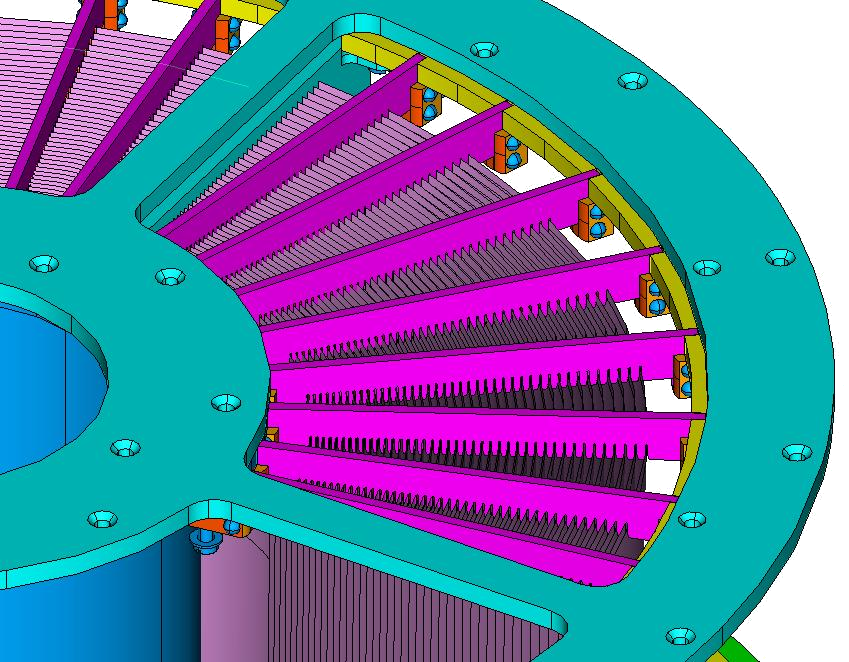
\includegraphics[width=0.9\linewidth, height=5cm]{SXT_foil_mount.png} 
\caption{SXT Foil Mount}
\label{Foil Mount}
\end{subfigure}
\begin{subfigure}{0.3\textwidth}
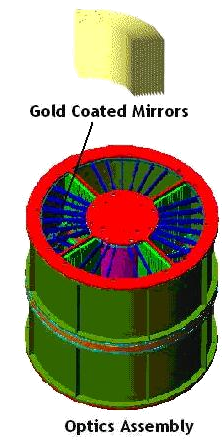
\includegraphics[width=1.0\linewidth, height=6cm]{SXT_OPTICS.png}
\caption{SXT Optics Assembly}
\label{Optics Assembly}
\end{subfigure}
\caption{SXT foil mount and optics assembly}
\label{fig:Optics assembly}
\end{figure}
\paragraph{}
A schematic of the SXT reflector is as shown above, with the diagram of the SXT Foil Mount. The upper half consists of the $1$-alpha section and the lower half consists of $3$-alpha section.
\subsection{Focal Plane Camera Assembly}
\paragraph{}
\begin{wrapfigure}{r}{0.5\textwidth}
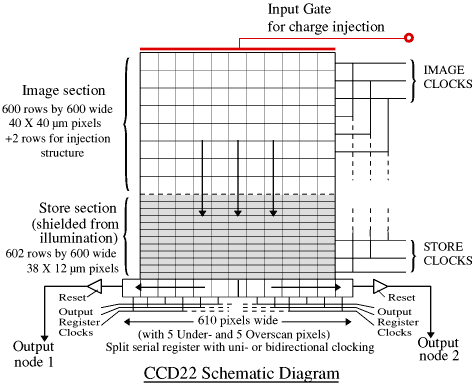
\includegraphics[width=1.0\linewidth]{CCD22.png} 
\caption{}
\label{fig:CCDSD}
\end{wrapfigure}
The focal plane camera, the instrument responsible for collecting the data is a thermo-electrically cooled (by the Peltier effect) X-ray CCD camera, similar to the one flown in the XMM and SWIFT missions. The CCD dimensions are of $600$x$600$ pixels each pixel being $40$ square microns. It is a frame transfer device, i.e. an image transferred from image to store section can be read out while a new image is being acquired. 
\paragraph{}
The CCD operates in single photon counting mode. Each X-ray photon, depending on the energy liberates about $100$-$1000$ electron hole pairs. Preserving this total charge information for each photon will lead to the measurement of its energy, thus enabling spectroscopic studies. The energy resolution is strongly degraded by system noise. So in order to reduce the thermal noise in the CCD it is thermo-electrically cooled to an operating temperature of $193$ $K$, which is expected to yield an energy resolution of $0.02$ at $6$ $KeV$.
\paragraph{}
The focal plane camera assembly consists of the CCD and its cooling arrangement housed in a cryostat, which also contains Iron-$55$ calibration sources (at the four corners of the CCD), an optical blocking filter for the CCD and an aluminum proton shield to protect the shield from proton damage while passing through the south Atlantic anomaly region. The optical blocking filter is made of a single fixed polyamide film of $184$ mm thickness, with a $48.8$ $mm$ thick aluminum coating on one side. This yields an optical transmission of about $0.0025$, limiting the background light reaching the detector. The entire cryostat body is made of aluminum alloy, and gold plated for thermal insulation.
\begin{wrapfigure}{l}{0.6\textwidth}
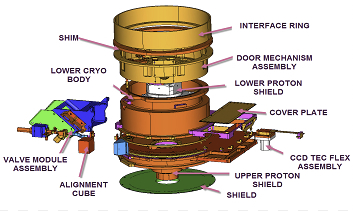
\includegraphics[width=1.0\linewidth]{IMp2.jpg} 
\caption{SXT CCD Module}
\label{fig:CCD Module}
\end{wrapfigure}
\subsection{Data Collection Modes}
\paragraph{}
The data from SXT CCD are stored on-board, and transferred to the ground station once each orbit (with an orbit of $\approx 97$ minutes each $14$ times a day). The memory quota for each orbit is $280$ $MB$. Hence this puts serious load on the data modes and how the data is packaged. There are four data modes, and only one mode for housekeeping. In each mode, the data is packed in $2$ $KB$ segments. Hence, the SXT memory per orbit is filled with $143360$ $2KB$ blocks. 
\paragraph{}
The various data modes are as follows:
\begin{description}
  \item[$\bullet$ Mode 1] Photon Counting (PC)
  \item[$\bullet$ Mode 2] Fast Windowed photon counting (FW)
  \item[$\bullet$ Mode 3] Bias Map (BM)
  \item[$\bullet$ Mode 4] Calibration Mode (CM)
  \item[$\bullet$ Mode 5] Housekeeping mode (HK)
\end{description}
\begin{wrapfigure}{r}{0.45\textwidth}
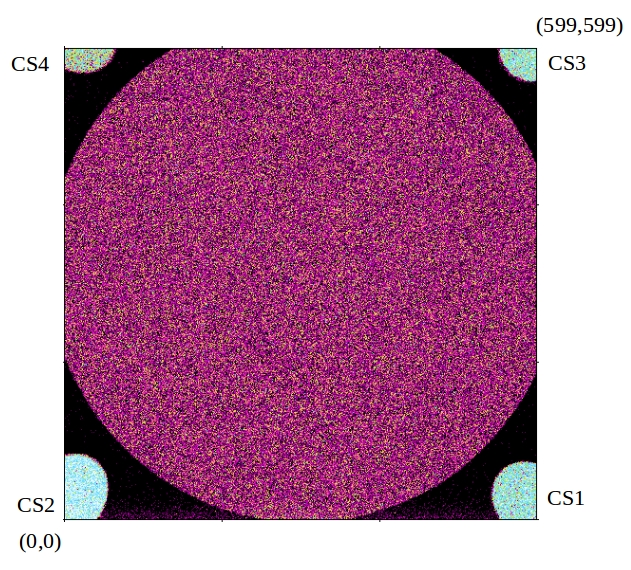
\includegraphics[width=1.0\linewidth]{SXT_calibration.jpg} 
\caption{SXT Calibration Sources}
\label{fig:SXT_Calibration}
\end{wrapfigure}
\subparagraph{Photon Counting Mode (PC):}
In PC mode, data from the entire CCD is collected, provided that these are above a specified threshold energy (set by the SXT team, it can be around $100$-$200$ $eV$). Currently it is about $105$ $eV$ (which is $4$ sigma above the noise peak). The readout time of this mode is \textbf{~2.4} s (that is, the amount of time it takes to read the data from the sensor).
\subparagraph{Fast Windowed photon counting mode (FW):}
In the FW mode, a $150$x$150$ pixel window is used at the center of the CCD. The readout time of this mode is ~$248$ $ms$ (hence FW mode has higher time resolution than PC mode). Data in the FW mode is also thresholded as in the PC mode. 
\subparagraph{Bias Map mode (BM):}
In the BM mode, the entire CCD frame is sent (again with zero threshold) with incrementally addressed $60$ rows per CCD frame along with their coordinates. On the ground, each of these frames are mapped to generate an individual CCD frame. It takes $24$ seconds of data to generate one fully mapped CCD frame.
\subparagraph{Calibration Mode (CM):}
The calibration mode, as the name suggests, is used to check the calibration of the SXT. The readout time of the calibration mode is ~$2.4$ $s$. Data from the four corner windows of the CCD with a size of $80$x$80$ pixels and a central window with a size of $100$ pixels are transmitted with zero threshold in the calibration mode. 
\subparagraph{Housekeeping mode (HK):}
The housekeeping mode is activated only when there is a failure of both LBT telemetry channels. When HK mode command is sent to SXT, LBT telemetry data in the form of HK data is sent in $2K$ data packages. Hence only one frame will be generated and pushed in currently operating mode data package. 
\subparagraph{}
Spectral information is available under all four modes. However, for this particular project I would be using only the first two modes, that is FW and PC mode for the data analysis. These are the modes that one uses to derive scientific data.  
\subsection{Data Levels of SXT}
SXT has three levels of data:
\begin{description}
\item[$\bullet$ Level $0$ data:]
These are the instrument-wise raw data in binary format, which are paired with its associated auxiliary data, which is segregated from all instrument combined raw data obtained through telemetry. This data is very mission specific and is not available for public use.
\item[$\bullet$ Level $1$ data:]
This data is obtained by applying various transformations on the level $0$ data and are stored in FITS format. The data is made available for public use only after an initial lock-in period. The Principle Investigator of the data will be given access to this data at the earliest possible time after a pre-processing to level $2$ and a check-out by SXT POC team. The Level-$1$ data directory contains science data file, time calibration file, attitude file, orbit-file, level-1 MKF file and house-keeping data file.
\item[$\bullet$ Level $2$ data:]
This data contains the standard science products obtained from processing Level $1$ data for a default set of parameters and is hence available for public use. The Level $2$ software offers user interface for proper selection of parameters and desired analysis of Level $1$ data. One can have selections of these parameters depending on  science objectives. 
\end{description}
\paragraph{}
Once we obtain the Level $2$ data, we can start with the “science” part of the project. That is discussed in detail later in the report. 
\newpage
\section{Introduction to the Large Area X-ray Proportional Counter}
\paragraph{}
LAXPC covers an energy range of $3$-$80$ $KeV$. The three LAXPC units aboard the ASTROSAT have the largest effective area (for collecting data) and sensitivity among all the satellite missions flown so far for X-ray astronomy studies above $20$ $KeV$, The instrument also has a fine time resolution of 10 microseconds. The collection area of the instrument is $8000$ $cm^2$. It is well suited for timing and spectral measurements. 
\paragraph{}
\begin{figure}[h]
\begin{subfigure}{0.6\textwidth}
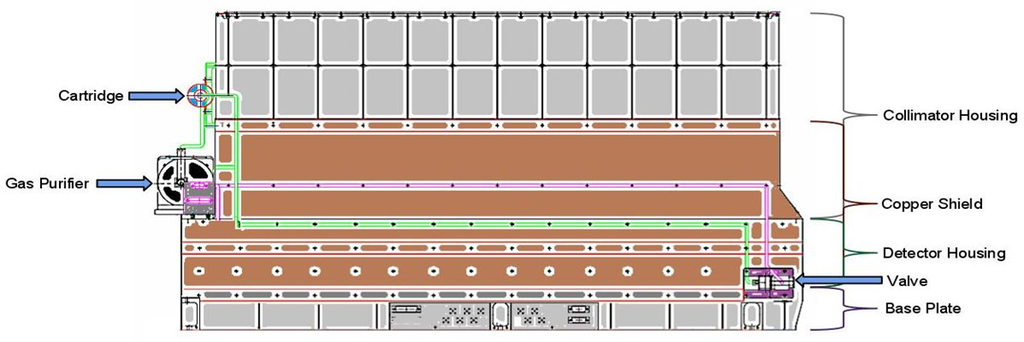
\includegraphics[width=1.0\linewidth, height=5cm]{image297_small.png} 
\caption{LAXPC Schematic}
\label{lAXPC Schematic}
\end{subfigure}
\begin{subfigure}{0.36\textwidth}
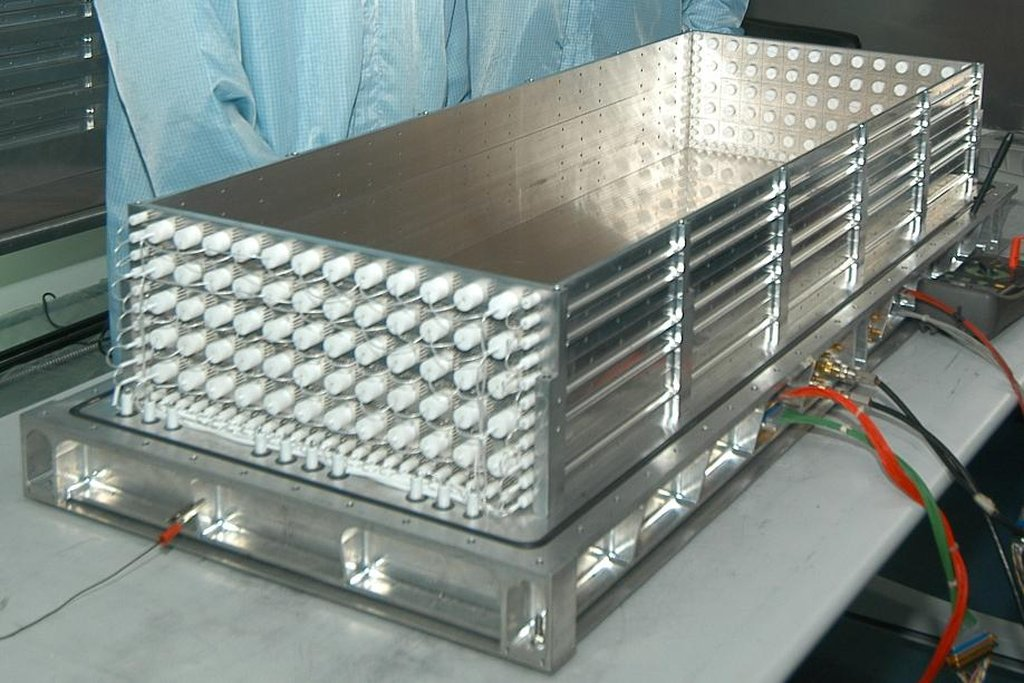
\includegraphics[width=1.0\linewidth, height=5cm]{image298_medium.jpg}
\caption{LAXPC Anode wiring}
\label{Anode wiring LAXPC}
\end{subfigure}
\caption{}
\label{fig:LAXPC}
\end{figure}
Because of the large detection volume (with a depth of $15$ $cm$) of LAXPC, and because they are filled with Xenon gas at $2$ atm pressure, the detection efficiency is greater than $50$\% in $30$-$80$ $KeV$ band. Hence the three LAXPC units will have the largest effective area and sensitivity among all the satellite missions flown so far.
\paragraph{}
Each LAXPC detector consists of $60$ anode cells with a  $3$ $cm$ $\times$ $3$ $cm$ cross section with a length of $100$ $cm$ arranged in $5$ layers providing a $15$ $cm$ deep X-ray detection volume. Hence each anode layer has $12$ anodes with a total width of $36$ $cm$. A Veto layer made up of $46$ anode cells each with cross-section of $1.5$ $cm$ $\times$ $1.5$ $cm$ surrounds the main X-ray detection volume on $3$ sides to reject events due to charged particles and interaction of high energy photons in the detector. 
\paragraph{}
\begin{wrapfigure}{l}{0.7\textwidth}
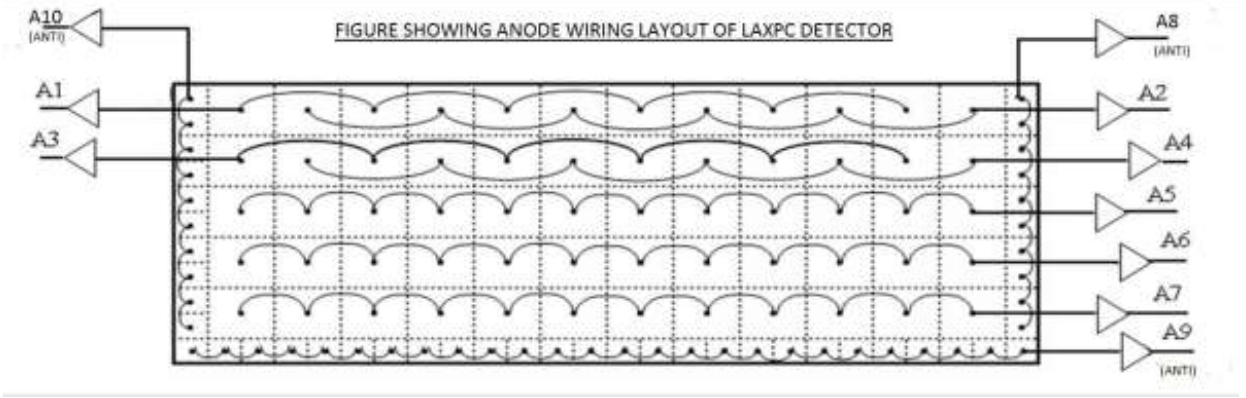
\includegraphics[width=1.0\linewidth]{Anode_wiring_layout_LAXPC.jpg} 
\caption{Anode wiring layout of LAXPC}
\label{fig:Anode wiring layout LAXPC}
\end{wrapfigure}
The alternate anode cells of Layer $1$ and $2$ are linked together and thus $4$ outputs are obtained from Layer $1$ and Layer $2$. The anode cells in each of the Layer $3$, $4$ and $5$ are linked together to provide one output from each layer. Thus, there are $7$ anode outputs that are operated in mutual anti-coincidence to reduce the non-cosmic X-ray background. The Veto layer is divided in $3$ parts providing $3$ Veto layer outputs. The left side and right side Veto anodes are linked together to provide one output from each one and the third Veto output is from the bottom layer Veto anodes linked together.
\paragraph{}
To suppress background from charged particles from all events, which register in multiple anodes, or those, which trigger the Veto anodes are rejected, except for the situation where one of the energies is in the K X-ray for Xenon. For X-rays with energy above the K-edge of Xe, a K-electron may be ejected and the ion can radiate a K X-ray photon in energy range $29.4$ - $34.4$ $keV$. These X-ray may escape from the detector or be absorbed in a different anode. In order to include such events the anti-coincidence logic is modified to detect this energy range. If two main anodes register an event and at least, one of them is in the energy range, of $25$-$35$ $keV$, then the energy of the two anodes are added and the event is accepted. The lower (KLLD) and upper (KULD) threshold can be set through tele-command.
\paragraph{}
The detector is filled with a mixture of $90$\% Xenon added with $10$\%  Methane at a pressure of $1520$ $torr$ (i.e. $2$ $atm$). The Mylar window is supported against the gas pressure by a honeycomb shaped collimator made of square geometry aluminum cells termed as Window Support Collimator (WSC). The Field Of View Collimator (FOVC) is placed above the WSC and is aligned with the openings in the WSC. The FOVC is made of sheets of tin, copper and aluminum and is placed in a collimator housing. The total height of the collimator is about $45$ $cm$ giving a Field of View (FOV) of about $0.9^o$ $\times$ $0.9^o$. A $1$ $mm$ thick tin sheet coated with copper serves as the shield for X- rays entering the detector from the sidewalls.
\subsection{Processing Electronics}
\paragraph{}
There are $7$ anode outputs from the X-ray detecting cells and $3$ Veto outputs from each detector that are fed to $10$ Charge Sensitive Per-Amplifiers (CSPAs). High voltage is supplied to the anodes from a command controlled HV unit whose output can be varied by another command. The $7$ X-ray anode and $3$ Veto layer outputs forming the CSPAs are sent to the peak detectors and events satisfying the selection logic as “true X-ray events” are further processed by signal processing electronics for Broad Band Counting (BBC) and time tagging every events with its energy to an accuracy of $10$ $\mu s$.
\paragraph{}
In BB counting output Anode $1$ and $2$ are combined as layer-L$1$, similarly Anode $3$ and $4$ are combined as layer–L$2$ and Anode $5$, $6$ and $7$ are combined as layer–L$3$. All Anti anode A$8$, A$9$ and A$10$ are combined as anti-counter. All the events in each LAXPC above a lower energy threshold of $3$ $keV$ in main anodes (A$1$ to A$7$) (LLD), upper energy threshold of $80$ $keV$ in main anodes (A$1$ to A$7$) (ULD), all the three Veto layer counts are termed as Anti-counts, are recorded in separate counters.
\subsection{Modes of operation of LAXPC}
\paragraph{}
All the three payloads of LAXPC have identical operation modes. There are three different modes of operation and each instrument can be operated in more than one mode simultaneously.
\paragraph{}
The LAXPC data carries information about the cosmic X-rays detected with the instrument and it has three entries i.e. the time of detection, the energy (spectral channel) of the X-ray photons and the identity of the detecting element (detector/anode-layer) including double-identity in some cases. The signal then generated by the instrument after detecting the X-ray is processed and stored in any of the following modes:
\paragraph{Normal Operation mode:}
During this mode there are two modes running simultaneously and the data is acquired from each LAXPC.
\begin{description}
\item[$\bullet$ Broad Band Counting Data:]
This mode records the data in various energy bands with selectable time bins (all the events within a time interval selected would be replaced by an energy value representative of that interval, often being the energy value of the median time), in this case it is usually between 16 ms to 2048 ms. The default binning value is $128$ $ms$. There are $15$ counters for the broadband counting of the valid X-ray events in different energy bands covering $3$-$100$ $KeV$ from the three layers as mentioned above in the processing electronics section. Note that the bin time can be selected in multiples of $2$, and are done so by commands.
\item[$\bullet$ Event Mode Data]
In this mode, the energy and identity of each event is recorded. Also with a dead time of about $54$ $\mu s$, the arrival time of each microsecond is also tagged with an accuracy of $10$ $\mu s$. A total of $5$ $mb$ data is generated from each accepted and analyzed event.
\end{description}
\paragraph{Fast Counter Mode:}
In this mode the event rate is measured only from the top layer of the LAXPC counter in four energy channels covering $3$-$20$ $KeV$ band with a fixed time bin of $160$ $\mu s$. The dead time in this mode is $10$ $\mu s$. Each of the four counters are $8$ $bit$ deep and cover $3$-$6$, $6$-$8$, $8$-$12$ and $12$-$20$ $KeV$ energy bands. This mode is used for studying rapid variabilities during short duration flares 
%\newpage
%\section{Introduction to Cadmium Zinc Telluride Imager}
%\subsection{*Edit This*}

%\newpage
%\chapter{Rossi X-ray Timing Explorer (RXTE)}
%\section{A brief Introduction to RXTE}
%\paragraph{}
%Named after the astronomer Bruno Rossi, NASA's Rossi X-ray Timing Explorer (RXTE) was launched into low-Earth orbit on December 30, 1995. The main objective of RXTE was to probe the physics of cosmic X-ray sources by making sensitive measurements of their variability over time scales ranging from milliseconds to year. How these sources behave are a source of valuable information since they provide insight into objects such as white-dwarfs, Neutron stars, Black holes, Pulsars, etc. Given that RXTE can maneuver at speeds of upto 6 degrees a minute, it can be made to point at transient sources rapidly. 
%\paragraph{}
%On board are three science instruments: the \textbf{All Sky Monitor (ASM)}, which scans the entire viewable sky and measures the time histories of source intensities in three energy bands from \textbf{1.5--12.0 keV}; the \textbf{Proportional Counter Array (PCA)}, composed of five co-aligned Xenon detectors (PCUs) with a total collecting area of 6500 cm$^2$, most sensitive over the \textbf{2-25 keV} energy range; and the \textbf{High Energy X-ray Timing Experiment (HEXTE)}, two clusters of "phoswich" scintillation detectors that rock on and off source along mutually orthogonal directions for real-time background measurements, sensitive to high-energy X-rays from \textbf{15-250 keV} (refer \cite{RXTE_standardProducts}). 
%\paragraph{}
%Among these, ASM was and still is primarily used to detect transient sources. Whenever any X-ray burst is detected, i.e. it crosses a certain threshold (which determines whether or not the signal is because of background oscillations) from a certain location of the sky, RXTE slews to the localization coordinates set by the ASM for a detailed observation (similar to how SSM works in case of ASTROSAT). This is when the other two payloads PCA and HEXTE come into play. 
%\paragraph{}
%PCA has 5 xenon gas proportional counter detectors that are sensitive to X-rays from 2--60 KeV. The PCA has a large collecting area ($\approx$ 6250 cm$^2$). The PCA's pointing area overlaps with that of HEXTE increasing the collecting area by $\approx$ 1600 cm$^2$.
%\paragraph{}
%HEXTE extends the sensitivity of RXTE up to 200 KeV, so that together with the PCA, they make an excellent, high time resolution sensitive X-ray detector. 
%\subsection{Data Analysis}
%\paragraph{}
Information on events within the PCA detectors are handled by the Experimental Data System (EDS), a microprocessor-driven on-board data system. The EDS is capable of processing upto 500,000 counts per second, and time the arrival of individual X-rays to about 1 micro second. The data can then be collected in a number of different modes simultaneously. This facilitates collection and analysis of the data appropriate to different sources. 
%\paragraph{}
%The data from different EDS and HEXTE are kept in separate files. Form these files the user extracts light curves and energy spectra. Then by running it through some algorithms, the astronomer converts the measured quantities into physical quantities. 
%\paragraph{}
%Astronomers use light curves to analyze short-term or long-term changes in intensity of a source. Further analysis of the light curves may reveal the presence of periodicity or the make-up of complex variations. Such studies may yield the size of the object or of the orbit the object may be in around another body.
%\paragraph{}
%The energy spectra are analyzed by fitting the data with models of possible energy sources. Statistics determine how well each model fits the data and may be used to eliminate inappropriate models. Successful analysis may determine, for example, the amount of energy emitted by the object and the source of the energy emission. Emission or absorption lines found in the spectrum further measure the composition of material in or surrounding the object.











%\newpage
%\chapter{Some Basic concepts}
%\section{Statistical significance}
%\paragraph{}
%In the following chapters you would come across "sigma" ($\sigma$) value a lot as a sign of a successful detection of the source signal (or any other parameter measured)









\newpage
\chapter{Introduction to the software}
\section{HEASARC}
\paragraph{}
The High Energy Astrophysics Science Archive Research Center (HEASARC) is NASA’s designated multi-mission archive for cosmic astronomy datasets for observations in cosmic, Extreme Ultra-Violet (EUV), X-ray and gamma ray wavebands as well as for Cosmic Microwave Background (CMB) datasets. These kinds of rays are mostly studied by observatories on the orbit, since these wavebands are generally absorbed by our atmosphere (our atmosphere is opaque to these wavelengths). HEASARC holds EUV, X-ray and gamma ray data for $32$ observatories which have been operated over the last five decades. 
\section{HEASoft}
\paragraph{}
Now in order to analyze data from the SXT and LAXPC, one needs to clean the data obtained, since this is the introduction part we wouldn’t go into the details of how it is done, we would come to the process of extraction later in the report. However, once one receives the level $2$ data, out of the pipeline software for a respective mission, one would need the help of certain data processing software so as to be able to extract the required light curves, spectra, image etc. from the data. 
\paragraph{}
This is where software packages like HEASoft come in. HEASoft is a collection of several packages that are designed to analyze high energy data efficiently and in an user-friendly manner from HEASARC. We would be using several packages from HEASoft, to be more accurate, we would be using the packages from XANDU, which is a collection of high energy data analysis software.
\paragraph{}
The software packages we would use (for now) are Xselect and Xspec (primarily, apart from some other packages from HEASoft which we would use for plotting, listing etc.) which we would be using in order to obtain our initial calibration results.
\subsection{Xselect}
\paragraph{}
Xselect is a Command Line Interface (CLI) software responsible for the following functions:
\begin{enumerate}
\item Organize the input of data through the observation catalogue, and store it internally for easy use.
\item Accept intensity, phase, region, detector, grade, event file column, spectral, and timing filters, which will be applied to the event data.
\item Make good time intervals (GTI) by applying selection criteria to the Housekeeping and auxiliary filter data.
\item Extract images, light curves and spectra from the event data, using the entered filters, as well as the GTI created by the applied selections.
\end{enumerate}
\paragraph{}
In our analysis, we would be using several of the above functions in order to obtain our Good Time Intervals (GTI), apply several filtering to the data etc. We would discuss the steps to obtain meaningful data later in the report. One of the salient features of Xselect is that it can be configured to support any new mission or instrument that does not require any mission specific routines, simply by editing the mission database file Xselect.mdb. This makes Xselect a great tool to obtain the preliminary files needed for  spectral analysis, using the ASTROSAT data. 
\paragraph{}
Now, one might wonder, what is a GTI? GTIs are a table of sorted START and STOP times in units of seconds. The GTIs give the time periods when the mission time line parameters fell within acceptable ranges. In other words, the “good times” are those times when the observation conditions were “good”. Some of the principle reasons for bad observation period are $1$). Bad Aspect Solution (bad RA, Dec, roll angle of the telescope versus time), i.e. when the telescope isn’t tracking accurately in accordance with the change in RA and Dec while telescope slews, and $2$). 

High background times are when there is a surge of background events (meaning, cosmic rays or any other high energy rays, from sources other than the observed source hitting the sensor, which would generate an event that is not from the actual source being observed) and $3$) When the satellite passes through the South Atlantic Anomaly (SAA), this is a region where the earth's inner Van Allen Radiation belt comes closest to the earth's surface, and hence bombards anything (in our case satellites) with higher than usual dose of charged particles, causing problems such as reduced lifetime, corrupted data etc. from the satellite. One might wish to create a more restrictive set of GTIs if one wishes to reduce the background influence on the data. Now, one might ask how does one process the data obtained from the satellite? The satellite takes in all the data, everything while it is pointed to the object, even when the object is behind earth. The GTI filtering is done during the conversion of level $0$ to $1$ to $2$, at every step. However, even after the stringent filtration there could be some frames that are not quite right and might need further filtration during the data processing with Xselect, the process will be discussed with examples later in the report.
\paragraph{}
Now, to sum it up, we will be using Xselect, to obtain:
\begin{enumerate}
\item The spectral file, with an extension .pha (Pulse Height Amplitude). This file contains point based  count-histogram obtained from an X-ray observation. This type of spectral file is also called the type I PHA, (type II being .pi), which complies to the Office for Guest Investigator Programs (OGIP) spectral file format. This file represents the integrated charge per pixel from an event recorded in a detector. In early electronic devices this was the size of the pulse recorded. This means, that if a high energy photon is “detected” (meaning, generates a pulse of current), this .pha file is carrying the information of the current generated by this photon, i.e. information of its energy. Note, on getting this file, one loses the timing data.
\item The Light Curve (.lc) file, which, as the name suggests, contains a map of the intensity of X-rays photons received from the source as a function of time. This helps us study the variation of the intensity of the source with respect to the time. In easier terms, light curves are graphs that show the brightness of an object over a period of time. 
\item The events list, with an extension .evt . X-ray instruments record a separate signal from every individual photon they detect. This is unlike optical CCDs which need to integrate the signal from a number of photons to generate a detectable signal. As a result X-ray data is stored event by event, retaining more information allowing for greater flexibility of analysis. Every X-ray “event” (a general term for a detection, may refer to a photon or a background cosmic ray) is characterized by a pulse height that encodes the energy of the incoming photon, a time coordinate (which details when the pulse was detected), a grade (a number assigned to every event, based on the number of pixels in its immediate surrounding i.e. $3 \times 3$ pixels, which have crossed their threshold value), and typically two position coordinates (meaning, from “where” this signal was detected). One might think of the events list as a $4$ dimensional array of x, y, time, energy. However, since most of the pixels are empty, an event would be a collection of non empty pixels. Also note that there are many more parameters for each photon (event) than just these $4$. 
\item The Image file with an extension .img . These are the images of the event files of the whole field and/or an expanded view of the central region. 
\end{enumerate}
\paragraph{}
Note that this just an introductory paragraph for Xselect, we would discuss the commands we use to extract meaningful (i.e. data from which we can draw scientific meaning) data later in the report.
\subsection{Xspec}
\paragraph{}
Xspec is a command driven, interactive, X-ray spectral fitting program, designed to be completely detector-independent so that it can be used for any spectrometer, the key word being “fitting”. Although we use a spectrometer to measure the spectrum of the source, what we receive is not the spectrum, but the photon counts (C) within specific instrument channels (I). This observed spectrum is related to the actual spectrum of the source f(E) by (ref. *insert citation for xspec manual*): 
\begin{equation}
C(I)=\int{f(E)R(I,E)dE}
\end{equation}
\paragraph{}
Where R(I,E) is the instrument response and hence is proportional to the probability that the incoming photon will generate an event of energy E detected by the channel I. Ideally, we would think that inverting the equation would give us the f(E) for a given set of C(I), however, doing so makes f(E) get solutions that are non unique and unstable to small changes in C(I). 
\paragraph{}
Another alternative would be to choose a model spectrum f(E), that can be described in terms of a few parameters and match, or “fit” it to the data obtained by the spectrometer. For each f(E), a predicted count spectrum $C_p (I)$ is calculated and compared to the observed data C(I). Then a “fit statistic” is computed from the comparison and used to judge whether the model spectrum “fits” the data obtained by the spectrometer.
\paragraph{}
The model parameters are then varied to find the parameter values that give the best fit statistic. These values are, as one might guess, are referred to as the best-fit parameters. The model spectrum, $f_b (E)$, made of the best-fit parameters is considered to be the best-fit model.
\paragraph{}
The most common statistic used to determine the “best-fit” model is $\chi^2$, defined as follows (ref. *insert xselect manual reference here*):
\begin{equation}
{\chi ^2} = \sum \frac{(C(I) - C_p (I))^2}{(\sigma (I))^2}
\end{equation}
where $\sigma (I)$ is the (generally) unknown error for channel I. 
\paragraph{}

Now, how can we say, with the help of $\chi ^2$, that the particular model is best-fit? This is where the goodness-of-fit comes in. The $\chi ^2$ statistic provides a well-known-goodness-of-fit criterion for a given number of degrees of freedom ($\nu$, which is calculated as the number of channels minus the number of model parameters) and for a given confidence level. If $\chi ^2$ exceeds a certain critical value one can conclude that $f_b (E)$ is not an adequate model for C(I) i.e. the observed data. As a general rule, one wants the value of reduced $\chi ^2$ (i.e. $\chi ^2 / \nu$) to be approximately equal to one. That is, $\chi ^2$ is approximately equal to $\nu$. A reduced $\chi ^2$ greater than one indicates a poor fit, while a reduced $\chi ^2$ that is much less than one indicates that the errors in the data have been over estimated. Note that even if the best-fit model passes the “goodness-of-fit” test, it doesn't mean that $f_b (E)$ is the only acceptable model. For example, if the data used in the fit are not particularly good, one may be able to find many different models for which adequate fits can be found. In such a case, the choice of the correct model to fit is a matter of scientific judgment.
\paragraph{A point to note while choosing the model to be used}
Now, while choosing the appropriate model, there are many things that have an impact on the resultant data and hence would make a huge difference in what is being obtained at the end. A few things that one might do well to consider while choosing the model would be:
\begin{enumerate}
\item Look where the object is at, that would help you select whether you consider the galactic or photon absorption model. (do recheck)
\item (this section is under work and I will a
dd new models soon) 
\end{enumerate}
\paragraph{}
Another point which one would have to keep in mind would be to determine the " confidence interval ” for the parameter (i.e the range of values within which one can be confident the true value of the parameter lies). The confidence interval for a given parameter is calculated by varying the parameter value until $\chi ^2$ increases by a particular amount above the minimum, or best-fit value. The amount that $\chi ^2$ is allowed to increase (also referred to as the critical $\Delta \chi ^2$) depends on the confidence level one requires, and on the number of parameters whose confidence space is being calculated. The critical for common cases are given in the following table (from *insert reference here* Avni, $1976$) (ref. *insert xselect manual reference here*):
\begin{center}
\begin{tabular}{ |c|c|c|c| } 
 \hline
 Confidence & \multicolumn{3}{|c|}{Parameters}\\
 & 1 & 2 & 3\\
 \hline 
 0.68 & 1.00 & 2.30 & 3.50 \\ 
 0.90 & 2.71 & 4.61 & 6.25 \\ 
 0.99 & 6.63 & 9.21 & 11.30 \\ 
 \hline
\end{tabular}
\end{center}
\paragraph{}
We shall discuss the implementation later in the report. 
\newpage
\chapter{Setting up the system}
\paragraph{}
The software one is expected to have at their disposal in order to process the data from SXT and LAXPC are as follows;
\begin{description}
\item[$\bullet$ HEASoft]: As mentioned previously, we would be needing packages such as Xselect and Xspec for plotting the light curves and energy spectrum of the source we would be observing. We would also (occasionally) need f tools to be able to list the good time intervals, so that we can use them for time filtering the data.
\item[$\bullet$ SAO ds$9$]: It is a software that we would be using to plot the image of the source. We would be using it primarily for the SXT analysis since plotting the image for LAXPC doesn’t make logical sense. Why? Because of the way both these instruments collect data. Another important function of this software would be to generate the regions file so that we can perform region filtering with Xselect. And to get the RAWX and RAWY coordinates of the center of the object in the sensor. 
\item[$\bullet$ SXTEVTMERGERTOOL]: This, as the name suggests is a tool that we would be using to merge the clean event files from every orbit into one clean event file which would contain all of the data. The installation file is given in in the SXT POC website.
\item[$\bullet$ SXTMKARF] This is one of the many SXT pipeline tools that one might need install to obtain the off-axis auxiliary response files from the level $2$ (offaxis) .pha files with the help of the on-axis .arf files. 
\item[$\bullet$ LAXPC] Setting up the system to analyze LAXPC data requires one to run the FORTRAN codes mentioned in the downloaded software package. Note, that at the time of writing this report there were $2$ major software packages for analyzing the LAXPC level $1$ data. One is the base FORTRAN code written by H.M. Antia, which is available at the TIFR POC website, and the second one is the base code with a python shell, making it easier to use, and a cleaner interface. However, Dr. Antia's code is updated on December $21^{st}$ and contains the recent background processing software during the time of writing this report. The method for installing the software is given in the read me files with the package. 
\end{description}
\paragraph{}
Note that I have refrained from mentioning the installation steps of these software. I have done so because every environment has a different method of installation of the software and hence mentioning how I got them to work on my local system (which is a bash shell Ubuntu $16.04$ LTS system) would be futile since the instructions which I might mention here would only work if someone has the same system as my own. However, one thing to note is that to run the sxtevtmergertool and sxtmkarf, I would recommend the installation of pip, and, using that install several python packages such as scipy etc (to keep this report short, I haven’t attached a list of all the packages here). since they (i.e. sxtevtmergertool and sxtmkarf) would need those python packages as auxiliary support. Also, one might need to initialize HEASoft every-time one wishes to run those software in a new terminal.
\chapter{Data Processing}
\paragraph{}
This section would be divided into two parts, SXT data analysis and LAXPC data analysis. Since I have done SXT analysis to begin with, I would be discussing the basic steps to obtaining the light curves and energy spectra from the level $2$ data from SXT first. We would then move on to LAXPC analysis later in this section.
\section{SXT data Processing}
\subsection{Step 1: Merging the data}
\paragraph{}
In this section we would be discussing the steps to process the level $2$ data obtained through the SXT pipeline. For starters, since I have done the SXT analysis till date (of writing this report) we would be discussing SXT data analysis at the start. Assuming that all the above software are installed without any errors, let us look into the basic steps towards obtaining the light curves and the energy spectrum of the given level $2$ data. 
\paragraph{}
Now the level $2$ data that we were talking about comes in the following form (figure \ref{Crab_Compressed}) and when extracted they are as figure \ref{Crab_Extracted}. In order to save space the data is compressed. As mentioned above, I am using Ubuntu $16.04$ LTS (And this would work on any further versions as well) and hence, the screen-shots are from the same. Once you have the data in such form, see to it that you extract it to a single file. This will be essential to create a list of the clean event files as mentioned later in the report. 
\begin{figure}[h]
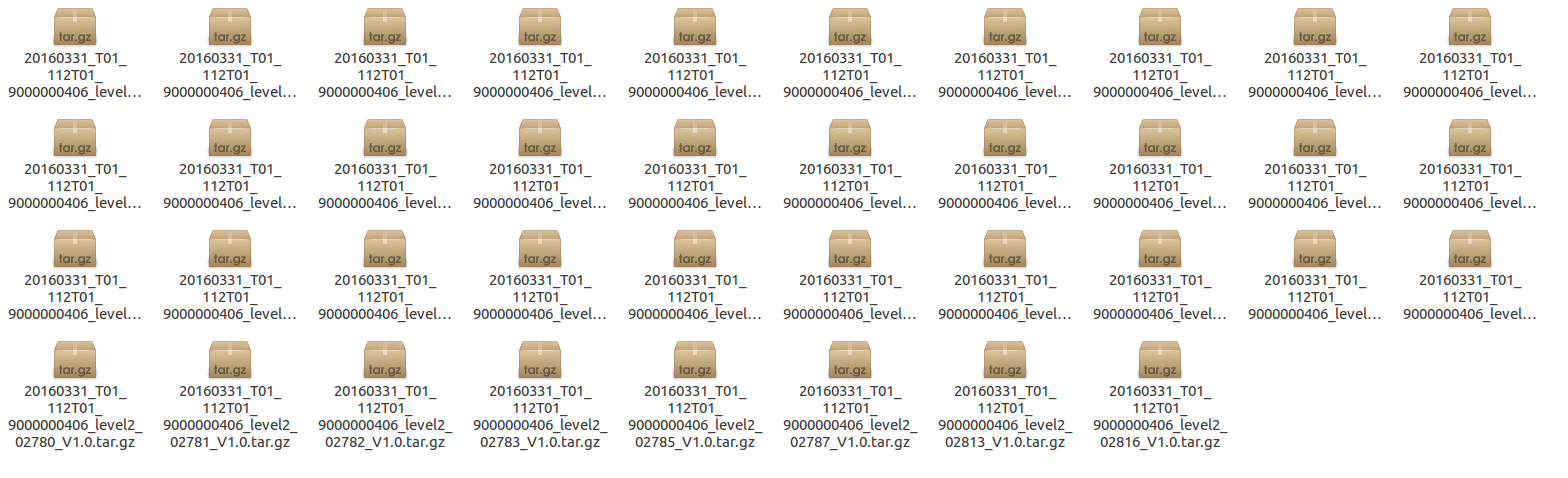
\includegraphics[width=1.0\linewidth]{Crab_Level2_Compressed.jpg} 
\caption{Compressed Data}
\label{Crab_Compressed}
\end{figure}
\begin{figure}[h]
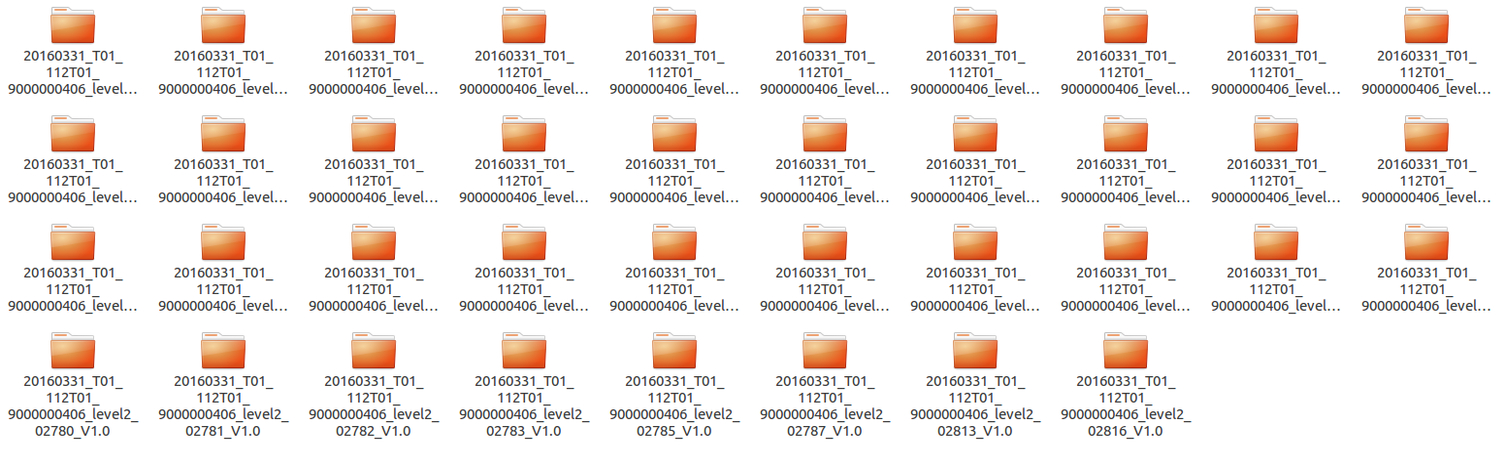
\includegraphics[width=1.0\linewidth, height=6cm]{Crab_Level2_Extracted.jpg}
\caption{Extracted Data}
\label{Crab_Extracted}
\end{figure}
\paragraph{}
Now, each of the extracted files is one orbit with their respective GTI(s). Now, as mentioned above, each of these orbits have their clean event files, which may have one or more GTIs, the reason for that could be because GTIs are those timings which are considered “good” for observation (i.e. timings when there is minimal background events, and good aspect solution), there could be several timings per orbit that would comply with those requirements and hence they will be included in the filtered file.  
\paragraph{}
However, we would have to merge those clean event files into one file so that we could use it in Xselect to obtain the .pha, .im, .evt, and .lc files. For that we would have to use the python script called sxtevtmergertool, as mentioned previously. Now, in order for sxtevtmergertool to work, it needs the location of all the clean event files in one .txt file. Now, there are two ways to do it, 
\begin{enumerate}
\item You copy and paste the locations of each clean event files manually, or,
\item You could let linux do all the work and have it create a list for you at the location where you wish. 
\end{enumerate}
\paragraph{}
Now, if you’re a fan of the good ol’ hard work then you are free to go for the first method. However, if like me, laziness is your forte you could use the second method to get the work done for you. Now, finding the clean event file is easy, 
\begin{enumerate}
\item Click on one of the files, eg. 
\item Go to the file \textbf{sxt}
\item There should only be one file in the folder, eg. \textbf{02740}. This is the orbit ID.
\item There should be two folders and one file in it. Click on \textbf{sxt.01}.
\item You would find many files in that folder. However, the file you are interested in has \textbf{cl.evt} at the end of its name.
\item Now, to copy the location of the file, just click on the file, then \textbf{ctrl+c}, then past it in any text editor. The location would look something like this, based on where you have your data.\\ 
\begin{center}
\path{/home/ankush/Desktop/Data/Level_2_Crab/Extracted/
20160331_T01_112T01_9000000406_level2_02740_V1.0/sxt/02740/sxt.01/AS1T01_112T01_9000000406sxtPC00_level2_cl.evt}
\end{center}
\end{enumerate}
\paragraph{}
Now, there are many aspects to the above location that changes, in every orbit, and certain aspects, such as \textbf{sxt}, \textbf{sxt.01} and \textbf{cl.evt} that remain same, (apart from the \path{home/ankush/Desktop/Data/Level_2_Crab/Extracted/}). Now, in order to make a list we would be using the \textbf{-ls} command. The syntax goes something like this:
\begin{center}
\item ls \path{/home/ankush/Desktop/Data/Level_2_Crab/Extracted/*/sxt/*/sxt.*/*_cl.evt} $>$ list\_name.txt
\end{center}
\paragraph{}
Notice that we have changed certain sections of the location and replaced them with * in the argument passed to ls. This tells the system to ignore changes in those “file names” and look for files with the mentioned (without *) names within them. The ls program would then make a list of all the files (in this case, the clean event files) that comply with the above given argument and save it to list\_name.txt in the directory where you are running this command. Note that sometimes the orbits have data in two different files, within the orbit folder, eg. sxt.$01$ and sxt.$02$ or more, this should be taken care for and we need those data as well, hence the * after the sxt. part, thus telling the computer to ignore the * part and take whatever files comply with the aforementioned name. 
\newpage
\paragraph{}
Now we have a list of all the clean event files which should look something like this when one opens the list.txt file. 
\begin{figure}[h]
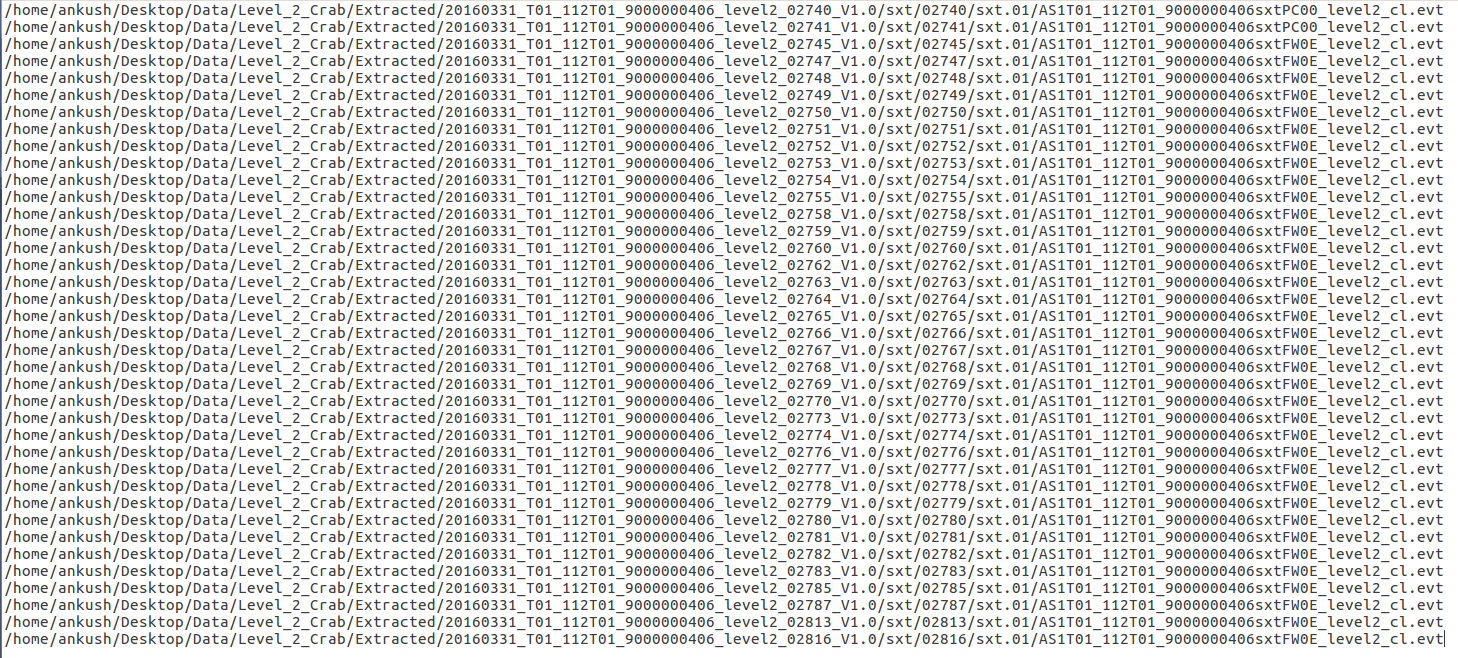
\includegraphics[width=1.0\linewidth, height=6cm]{Ls_all.jpg}
\caption{LS for all orbits}
\label{ls_all}
\end{figure}
\paragraph{}
Now, looking at the list screen shot, you might have noticed that the first two clean event files have \path{PC00_level2_cl.evt} written towards the end of the file name. And the others have \path{FW0E_level2_cl.evt} as their ending. This means the ones with PC are PC mode data and the ones with FW are FW mode data. {\large \textbf{Warning!! Do not merge PC and FW mode data together}}. Create a separate file for PC and FW mode (you could name them PC.txt and FW.txt, or however you like) and copy the PC mode lines to PC.txt and FW mode lines to FW.txt.
\paragraph{}
Now we can use these (PC.txt and FW.txt) with sxtevtmergertool to create a single clean event file for each mode to be able to use it in Xselect. Assuming that we have sxtevtmergertool installed properly, (one way to check that is to open the terminal and type sxtevtmerger -h command, on doing that we should get the help window of the sxtevtmergertool) we can use the command mentioned below to merge the files. 
\begin{figure}[h]
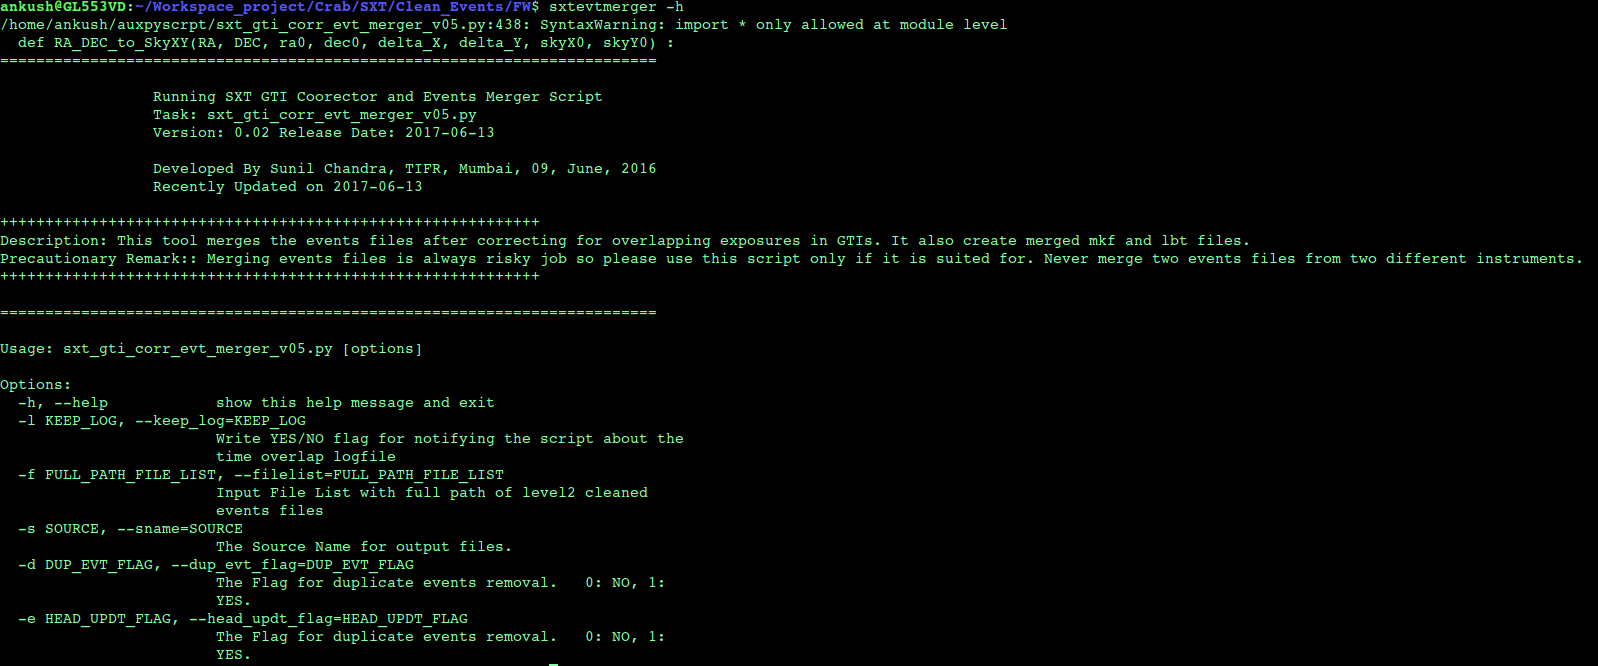
\includegraphics[width=1.0\linewidth, height=6cm]{sxtevtmergertool.jpg}
\caption{sxtevtmergertool help window}
\label{sxtevtmerger_help}
\end{figure}
\paragraph{}
Once we have confirmed that the merger tool is installed correctly, we can use the following command to get the clean event file for both PC and FW modes. 
\begin{center}
\item sxtevtmerger -f (location of the .txt file containing the list of all the cl.evt files) -s (name of the output cl.evt file)
\end{center}
\subsection{Step 2: Creating GTI list file}
\paragraph{}
Now that we have a Clean event file we are supposed to create a GTI time list file using the final clean event file.  We do this by using the FV command. We need to open a new terminal within the same working directory and type:
\begin{center}
\item \large \textbf {fv}
\end{center}
\paragraph{}
This will open a new window where it will first prompt us to open the cl.evt file we created in the previous section. We are supposed to open it, and the following dialogue box will open (Figure \ref{FV_one}):
\begin{figure}[h]
\begin{subfigure}{0.6\textwidth}
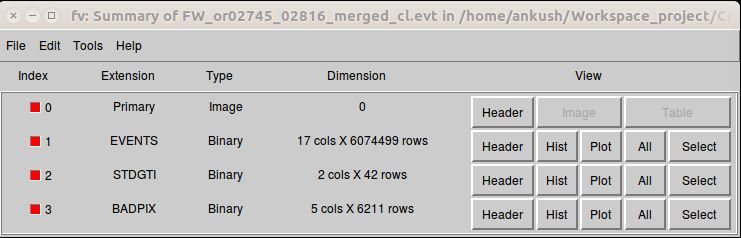
\includegraphics[width=1.0\linewidth, height=4cm]{Step_3.jpg} 
\caption{FV Clean Event file details}
\label{FV_one}
\end{subfigure}
\begin{subfigure}{0.36\textwidth}
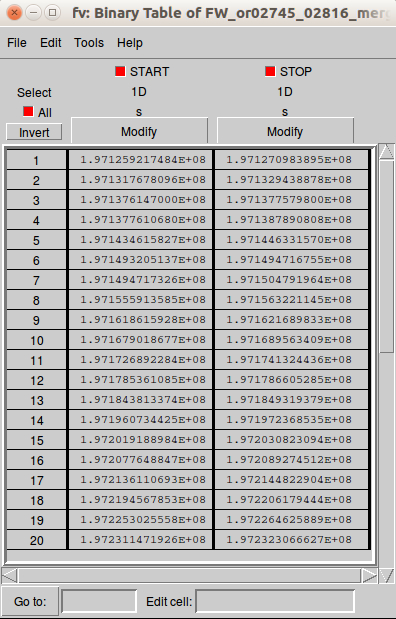
\includegraphics[width=1.0\linewidth, height=10cm]{Step_4.jpg}
\caption{FV GTI}
\label{FV_two}
\end{subfigure}
\caption{}
\label{FV_GTI}
\end{figure}
\paragraph{}
Now, in the third row, (index $2$) with the extension STDGTI, we are supposed to click on the all button on the right, under the column “view”. On doing that, we obtain Figure \ref{FV_two}. It is a list of all the Good time intervals in our clean event file. Notice that we had $36$ orbits worth of data, we got $42$ GTIs.  
\paragraph{}
\begin{wrapfigure}{l}{0.4\textwidth}
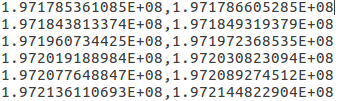
\includegraphics[width=1.0\linewidth, height=2cm]{Step_5.jpg}
\caption{Time File Format}
\label{step_5}
\end{wrapfigure}
Now that we have Figure \ref{FV_two}, we need to select, under "file" (in the tool-bar), the option to export everything as text. This will save this whole list of GTIs as a .txt file. Now, for the time filtering to work, it is advisable that we remove the inverted comma's from the intervals. It should look something like as shown in figure \ref{step_5} (Note, this is not all of the GTIs, just a small snapshot to display what format works with Xselect).
\paragraph{}
\newpage \clearpage
\subsection{Intermediate Step}
\paragraph{}
Instead of Filtering the file using the aforementioned method, another way of filtering would be to filter out bad orbits (and not GTIs, since each orbit might have more than one GTI intervals). The ultimate aim of this would be to make separate clean event files. There are two ways to do this. 
\subsubsection{Method 1}
\paragraph{}
When you enter Xselect, select the clean event file, filter using the command \textbf{filter time file} (given in the following section), and extract the event using the command (Xselect is given in the next section): 
\begin{center}
\large \textbf{extract event}
\end{center}
\paragraph{}
One can use \textbf{ext event} as well. Once executing the command Xselect would extract an event file, and you can then use that event to proceed with this file for further analysis (don't forget to save the event file!). This was one way of extracting the event. Another way (And the reason why this step is given here) would be to use the event merger tool to merge different orbits, without using xselect.
\paragraph{}
Now, the previous method does a similar thing since it creates separate clean event files for every GTI interval. What we would be doing in the second method would be to isolate the orbits in groups and use the merger tool on them, to get separate clean event files for every orbit group. How does one do that?
\subsubsection{Method 2}
\paragraph{}
From the initial orbit list file, the one that we made using the ls command in the previous section. Make equal groups of orbits each i.e. if you have a total of $40$ orbits, make groups of roughly $5$ orbits each (you can go more or less, since the main intention here is to make separate groups of more than one orbit). What do I mean by "make groups"? Well, create a new text file, and from the initial file (let us call that \textbf{file 1}), copy the first five (or whatever group size you have decided) lines, (note that each line is the location of one orbit, and sxtevtmergertool reads this, collects the files and merges them into one clean event file) and paste them in a new text file. Once done, select those text files and use sxt event merger tool on them to obtain clean event files for every bunch of orbits. 
\paragraph{}
Now, do this for both PC and FW mode. What you could expect to see is that in all of the, the image might be slightly off centered, or completely off centered. It will be more evident in the FW mode data than the PC mode data (However, you might see the skewed effect in the combined image Ref. Figure \ref{FW_PC_NT}). Now, once you have all the merged clean event files, plot them using Xselect, and look for offaxis, skewed images, etc. and eliminate those from your observation, i.e. never use them. Alongside the image, look for outliers in the light curve as well (the image and the light curves are extracted using the commands mentioned in the following section). Remember, if your image looks "good", but the light curve has outliers, those orbits cannot be used to proceed further. 
\paragraph{}
Now, the above step is crucial, and needs to be done repeatedly unless one has atleast five or so orbits that are: 
\begin{enumerate}
\item In continuity, no time gaps between them.
\item Has no outliers in the light curves
\item The central bright spot would be at the center, without any skew.
\end{enumerate}
\paragraph{}
Once done, the clean event file that you have will only need region filtering before you can extract the .pha, .lc, .evt, .im files, and whatever other file you need from the data. Further details given in the following section. 
\newpage
\subsection{Step 3: Xselect}
\paragraph{}
Now that we have separate clean event files for both FW and PC mode and we have the GTI list file, we can move ahead with Xselect. The steps of analysis for both PC and FW modes are the same, only with minor differences which I would mention as the need arises. Now, it is always advisable to use xselect and xspec in separate directories so as to avoid confusion, since both these software generate a lot of files that might create a cluster of files in the directory where you are working, However, that is just my approach, and is subject to debate. Remember to initialize HEASoft before using Xselect. 
\begin{figure}[h]
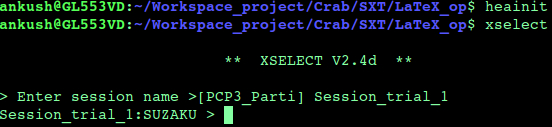
\includegraphics[width=1.0\linewidth, height=4cm]{Step_1.jpg}
\caption{Step 1}
\label{step_1}
\end{figure}
\paragraph{}
Once the Xselect terminal is open, Xselect will prompt you to enter the session name. This is just the name of the session and is up-to the user to decide the session name. In my case it was \path{Session_trial_1}. Remember space doesn’t work and hence \path{_} is advisable.
\paragraph{}
Now let us start by selecting the clean even file we made, for FW mode or for PC mode. The way we do that is to first use the command:
\begin{center}
\item \large \textbf {read event}
\end{center}
\paragraph{}
Xselect will then prompt us for the directory of the clean event file, here we are supposed to enter the directory location of the clean event file, and not the file itself, after which Xselect will prompt us again for the file name, which we are supposed to enter then. After which Xselect will prompt us to change the mission we are working on, to which we would answer ``yes" and get the following output:
\begin{figure}[h]
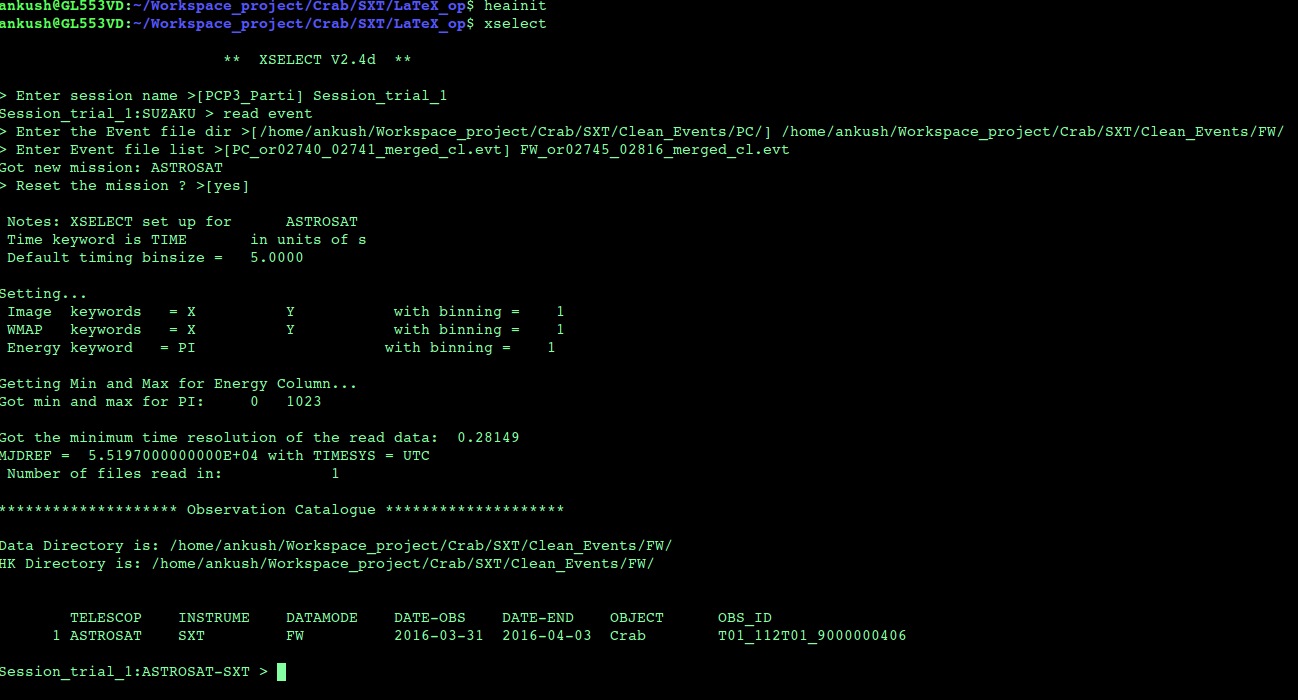
\includegraphics[width=1.0\linewidth, height=8cm]{Step_2.jpg}
\caption{Step 2}
\label{step_2}
\end{figure}
\paragraph{}
Now, we are ready to analyze PC/FW mode data. Up until now the steps are the same for both modes. First we would start off by extracting the data from the clean event files, data includes everything, i.e. img, evt, lc, pha, etc. files as we had discussed previously. The command to do that would be:
\begin{center}
\item \large \textbf {ext all}
\end{center}
\paragraph{}
This stands for extract all. The commands of HEASoft can be written in short form as well, as long as they are not ambiguous. So, extract all becomes ext all. Now, the first thing we need to check is whether the data is proper or not, we would do that by plotting the image using the command:
\begin{center}
\item \large \textbf {pl im}
\end{center}
\paragraph{}
Which means, Plot Image. This command would open a window of SAO ds$9$ and display the fits image there. The images one might get for starters might look something like this:
\paragraph{}
\begin{figure}[h]
\begin{subfigure}{0.5\textwidth}
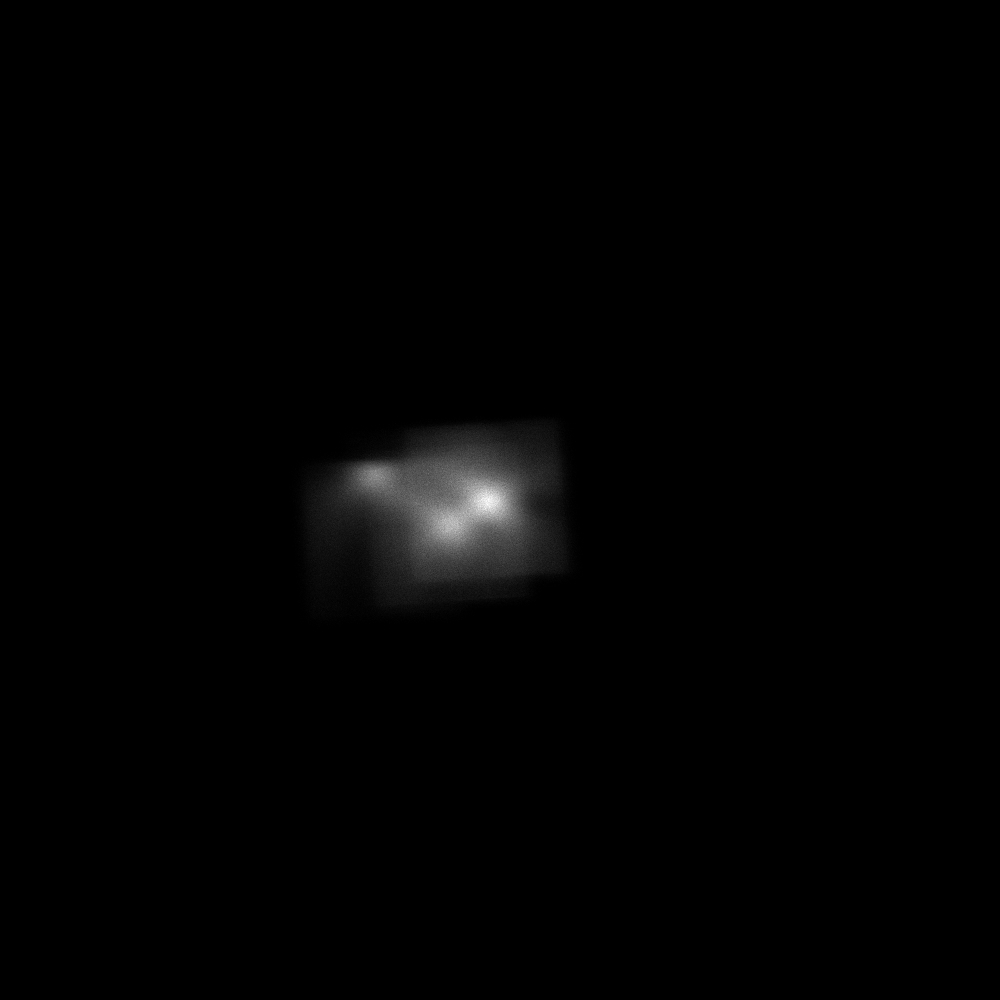
\includegraphics[width=1.0\linewidth, height=7.5cm]{FWF1_nt.jpeg} 
\caption{FW mode without time filter}
\label{FW_1}
\end{subfigure}
\begin{subfigure}{0.5\textwidth}
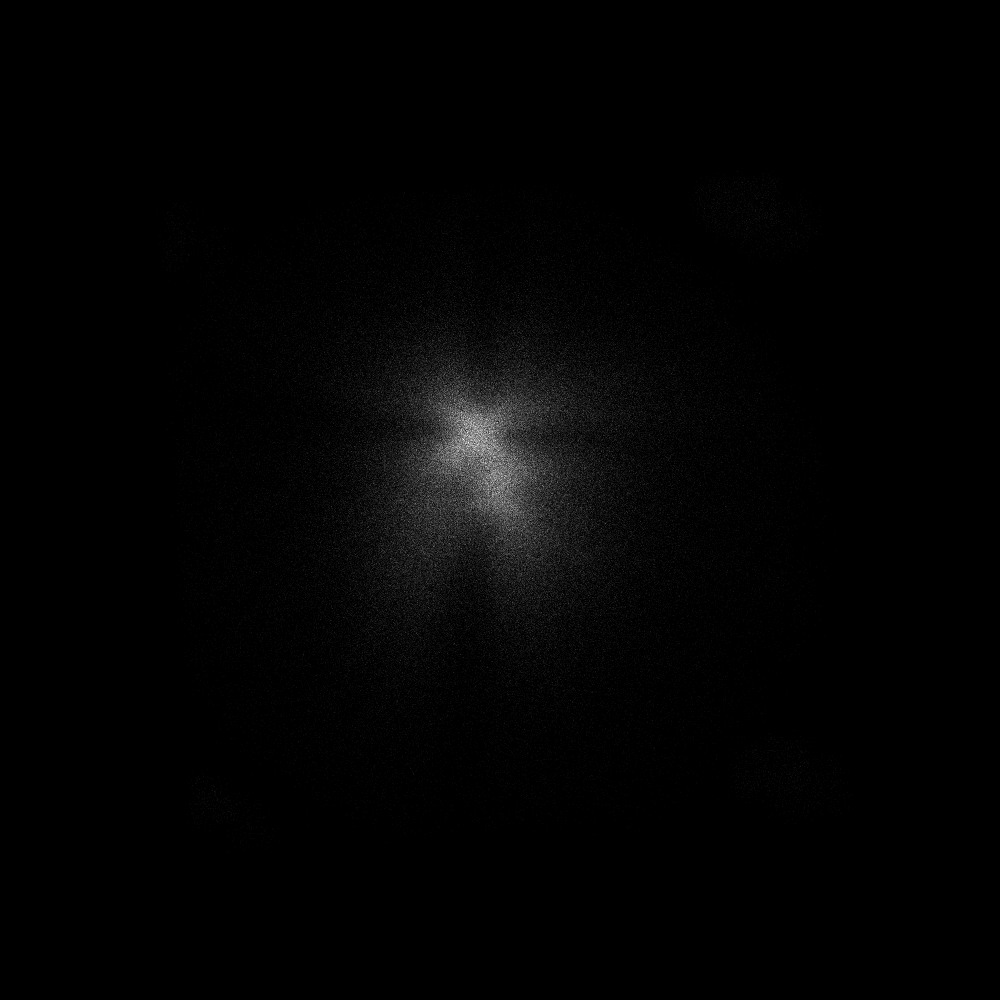
\includegraphics[width=1.0\linewidth, height=7.5cm]{PC_nofilt.jpeg}
\caption{PC mode without time filter}
\label{PC_1}
\end{subfigure}
\caption{}
\label{FW_PC_NT}
\end{figure}
\paragraph{}
Now, it is quite prominent by looking at the images that the data we have is skewed (some of the GTIs have bad aspect solution, hence they aren't, in essence ``Good" time intervals, based on the definition of aspect solution we discussed prior to this). i.e. There are certain GTIs in the list that are when the telescope wasn’t pointing towards the source, or, when the telescope hadn’t completed the slew to the object. However, we also see that there are certain GTIs that have the object at the center. We will be needing those GTIs. This is where it could get a bit tricky, since now, we are supposed to eliminate the bad GTIs. There are many ways of doing the said task. We could isolate different sets of GTIs by opening the time list file we got from fv, and select different sets of GTIs (first five GTIs become one set, the second five become the second set, so on and so forth), and save them in different .txt files. We do the same for both PC and FW modes. (note that it is not mandatory that we select GTIs in the sets of 5 only, we could take sets of $2$, $3$, $4$ etc. depending on the number of GTIs we have) A rule of thumb would be that since it is the initial stages of the observation that the telescope hasn’t slewed properly to the object, the initial GTIs have a higher chance of being skewed (however, it is not compulsory).Once we have the time files, we use the following command to filter out (filter every other GTIs out other than the ones mentioned in the list) the time interval:
\begin{center}
\item \large \textbf{filter time file (file name with path)}
\end{center}
\paragraph{}
Note that if you have followed the auxiliary step, section $4.1.3$, and have your own GTI filtered clean event file, then you need not further filter time using the above command (i.e. filter time). You can bypass this step, and move on to region filtering directly. 
\paragraph{}
Now, all the while we are filtering, we need to check the light curve as well, for the GTI set we are plotting. We plot the Light curve using the following command: 
\begin{center}
\item \large \textbf{pl curve}
\end{center}
The light curve, as mentioned previously, is a plot of intensity with time. If there are any intensity peaks in the light curve, it would suggest that the GTI where this peak occurs is a bad GTI. A good time interval from a bad time interval can be differentiated as follows: 
\paragraph{}
\begin{figure}[h]
\begin{subfigure}{0.48\textwidth}
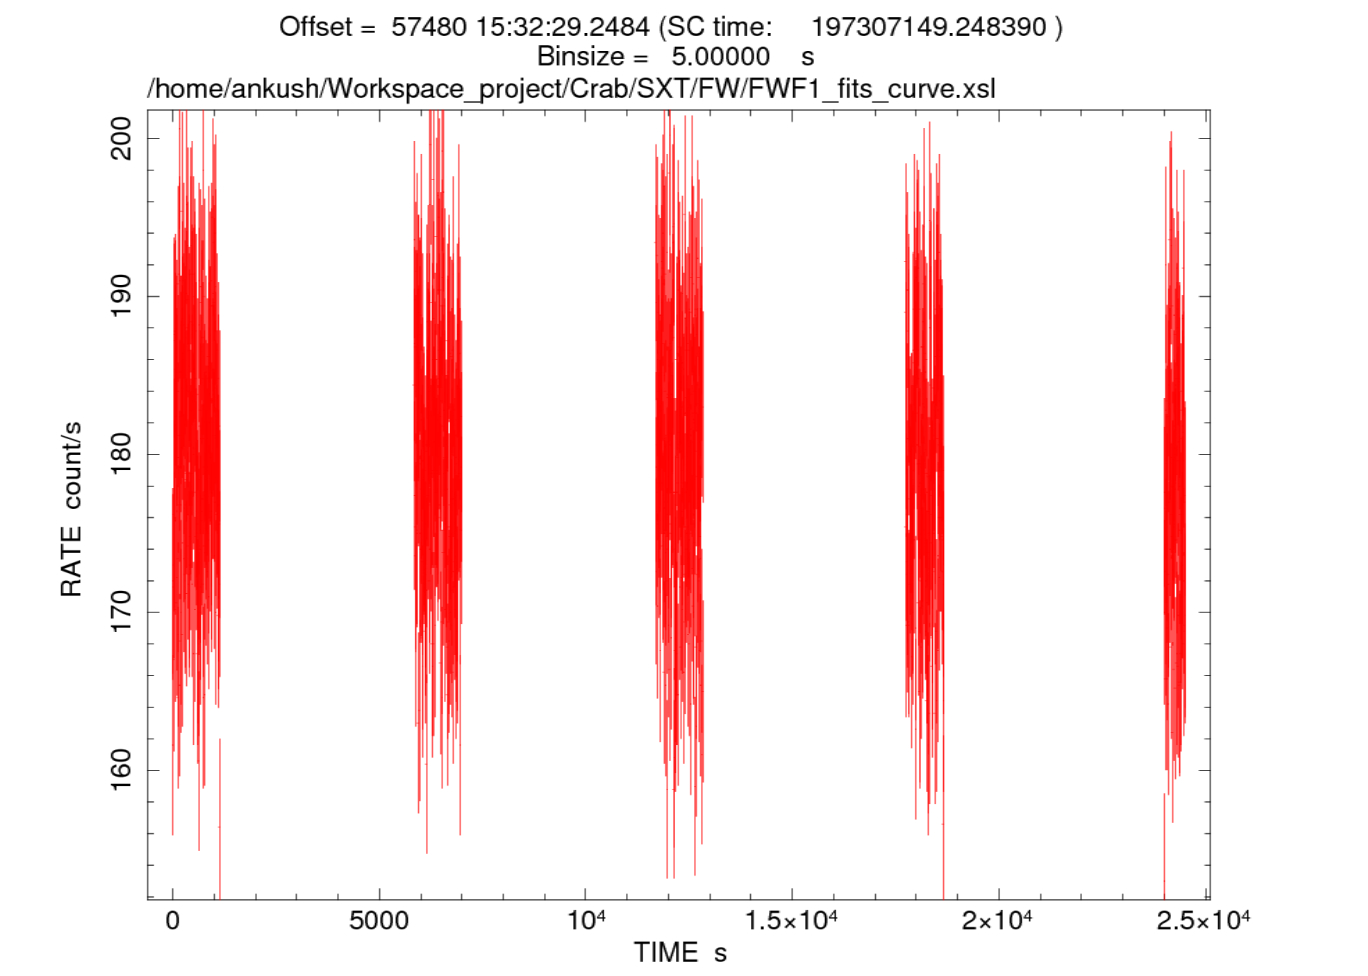
\includegraphics[width=1.0\linewidth, height=7.5cm]{Good_GTI.jpg} 
\caption{Good GTI Set}
\label{GTI_Good}
\end{subfigure}
\begin{subfigure}{0.48\textwidth}
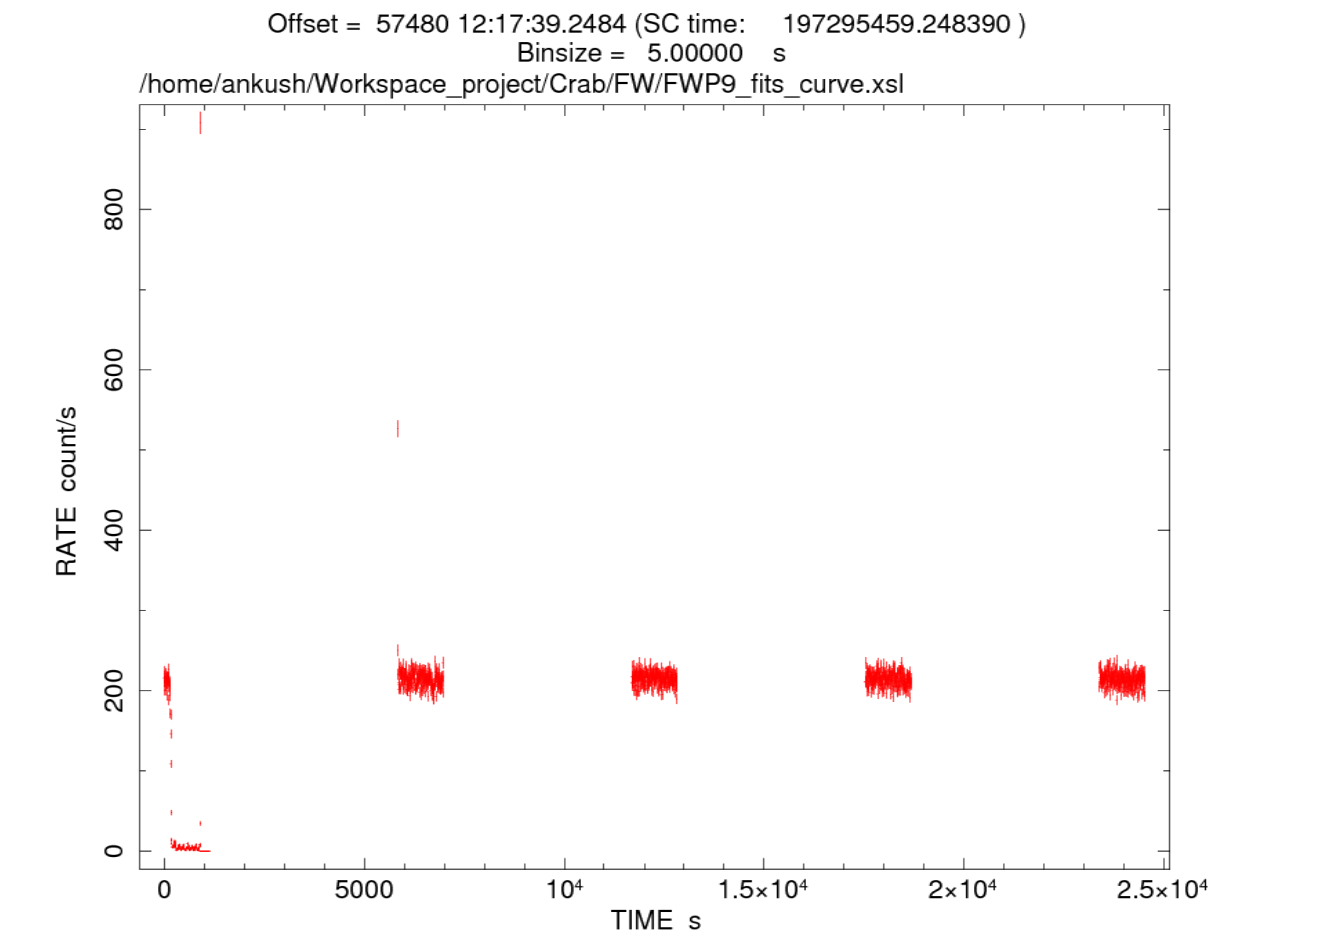
\includegraphics[width=1.0\linewidth, height=7.5cm]{Bad_GTI.jpg}
\caption{Bad GTI Set}
\label{GTI_Bad}
\end{subfigure}
\caption{The above is for FW mode data, as mentioned in the image itself}
\label{Good_And_Bad_GTI}
\end{figure}
\paragraph{}
After performing the GTI filter, we should now have a set of GTIs that are $1$). Not Skewed, and $2$). Do not have unnatural peaks in intensity (something that isn’t supposed to be there, however, the details are debatable, and beyond the scope of this report, for now).
\paragraph{A very important note:}
Given that you might end up eliminating majority of the data in this manner, this method would only be somewhat useful when you are trying to get the energy spectrum of the source. There are several things that could contribute to the sudden jumps in intensity, things such as thermonuclear bursts, among other things. However, such features can be seen across all devices and energy ranges. Hence, it is always advisable to compare the light curves across multiple devices if you wish to make sure that the features you are seeing are because of outliers and/or corrupted data. Also, longer duration features such as outbursts (in case of NS XRBs ref \cite{SB}) would also be visible in longer duration observations, and hence would not require one to alter the GTI selections.
\paragraph{}
After applying the necessary time filters, extracting everything and plotting the images again, should give us the output as shown in the figure \ref{Good_FW_and_PC};
\begin{figure}[h]
\begin{subfigure}{0.48\textwidth}
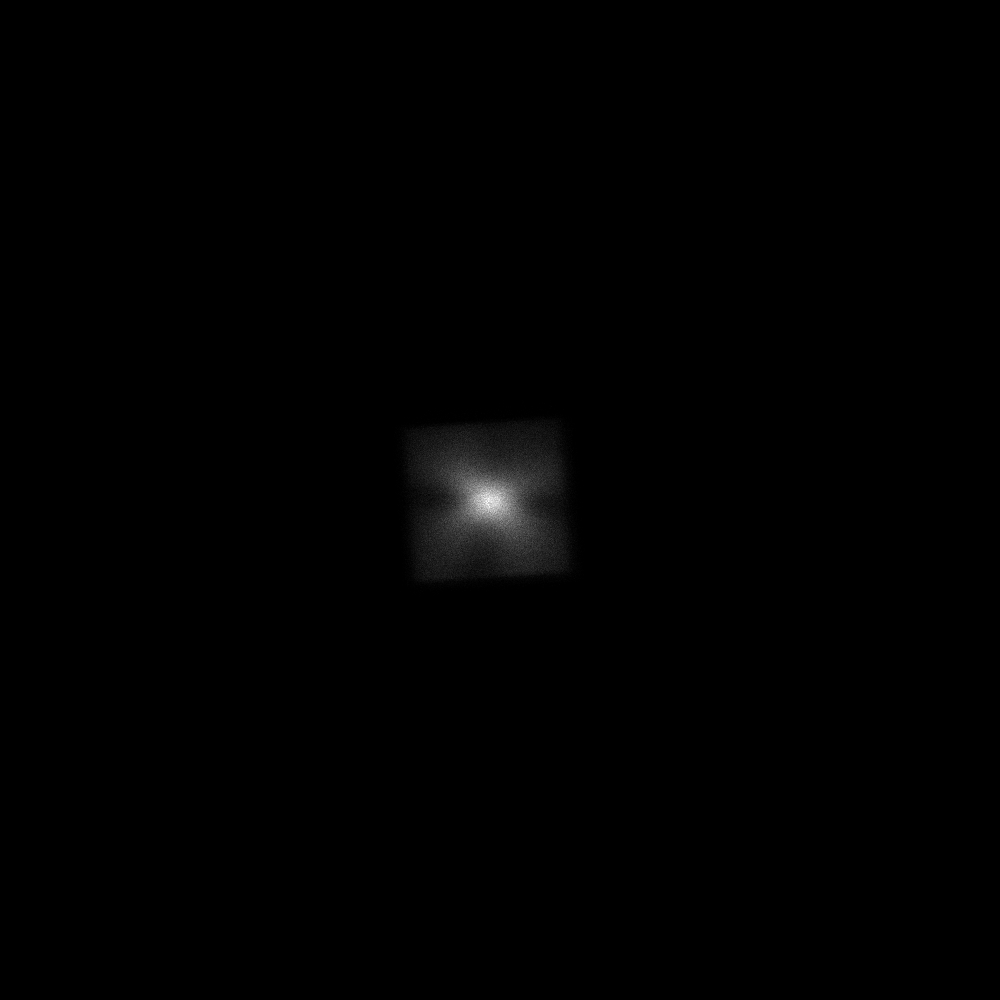
\includegraphics[width=1.0\linewidth, height=7.5cm]{FWF1_t.jpeg} 
\caption{FW mode with time filter}
\label{FW_Good}
\end{subfigure}
\begin{subfigure}{0.48\textwidth}
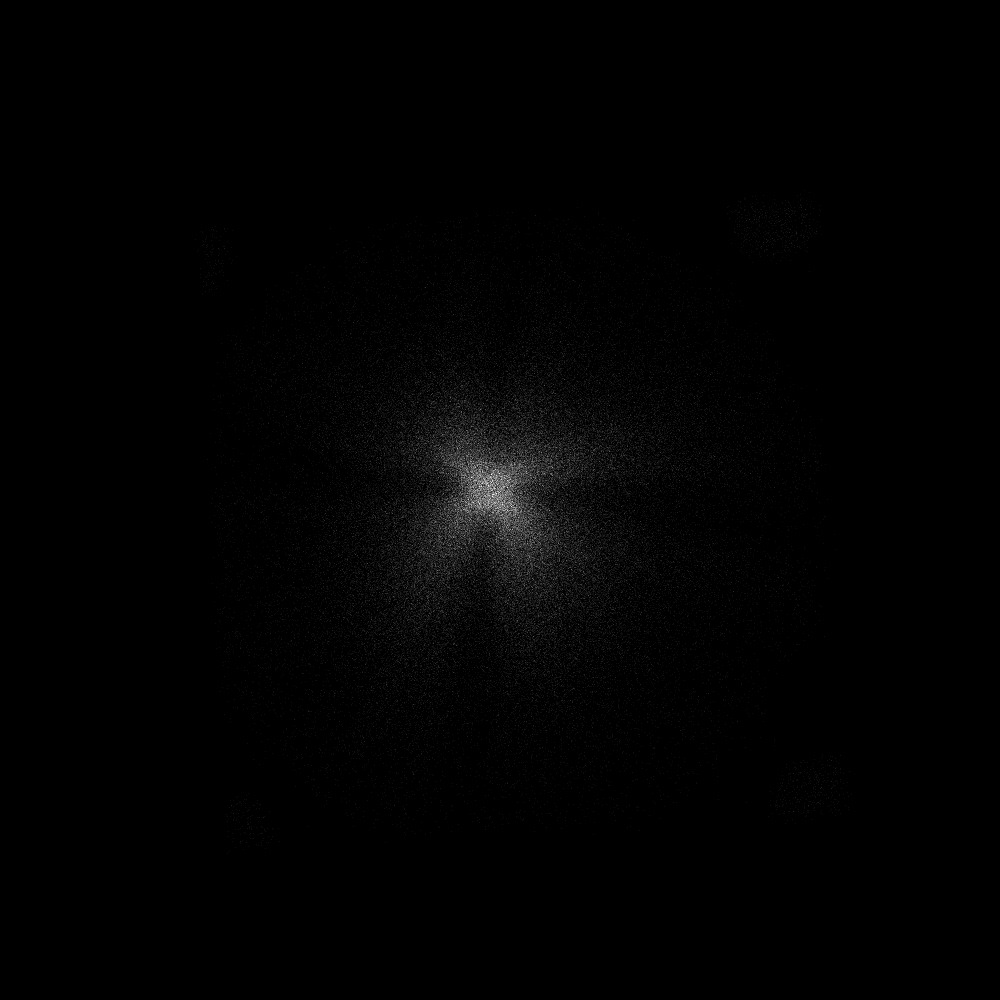
\includegraphics[width=1.0\linewidth, height=7.5cm]{PC_filt.jpeg}
\caption{PC mode with time filter}
\label{PC_Good}
\end{subfigure}
\caption{}
\label{Good_FW_and_PC}
\end{figure}
\newpage
\paragraph{}
Now that we are done with time filtering we need to apply region filters to the above before the output becomes usable with Xspec. In order to perform region filtering we first need a region file. A region file (with an extension .reg) is a two dimensional filter that can be used to include or exclude data from a given file. They are read and created using SAO ds9. In order to create regions file, we need to plot the image, click on edit, in the section where none is selected by default, select region, then in the same tool bar, click on region, a menu drops down, click on shape, and select annulus, i.e. a region of the shape of a ring, once done left-click on the image, and we should see a green (by default) color ring appear where we had clicked. Click on that ring, and now you can adjust the radius of both, the inner and outer circle of the ring. Once you have selected the ring, on the quick access panel, click on the region section, within which click on the information button. We would then see a small window pop up, which would give me the radius of the inner and outer circle in degrees. Click on the “degrees” button and select arcmin to display the radius in arc minutes (am). 
\paragraph{Note:}
Another thing that one has to take care about is that when selecting regions for PC mode, since you are selecting the regions manually, the centroid might not be the centroid of the image. In order to know the exact centroid coordinates (which will be used later in the SXTMKARF part), we need to click on the information button on the tool bar, which would open another window, with the x,y coordinates of the center, along with the radius values. Once done, click on the region drop down menu again, and select centroid. Ds9 will automatically try to detect the centroid of the image, since it is like a PSF, and hence would move the region's center to that location. Note down the centroid coordinates, and save the region. Keep doing this for every regions to get the best possible results.
\paragraph{}
Now, this is where we have different ways of selecting the regions. 
\paragraph{}
For FW mode, the regions have to be with;
\begin{enumerate}
\item $5$ $am$ outer circle radius and no exclusion from the center (using a circular region instead of an annulus) and,
\item $5$ $am$ outer circle radius with $1$ $am$ central exclusion. Meaning, the outer radius of the annulus is $5$ $am$ and the inner radius of the annulus is $1$ $am$.
\end{enumerate}
\paragraph{}
For PC mode, the regions have to be with;
\begin{enumerate}
\item $16$ $am$ outer circle radius and $1$ $am$ inner circle radius.
\item $16$ $am$ outer circle radius and $2$ $am$ inner circle radius.
\item $16$ $am$ outer circle radius and $3$ $am$ inner circle radius.
\end{enumerate}
\paragraph{}
Once generated, we need to save them with names discernible among other region files. Now, we would have to apply these region filters using the command:
\begin{center}
\item \large \textbf{filter region (file name of the region file with .reg extension)}
\end{center}
\paragraph{}
Note; to avoid bugs in the output files, it is advisable to apply one region filter, save the output (discussed later), quit, open xselect again, open the clean event file, use the time filter that was selected previously as the Good GTI filter, then apply the second filter, save, rinse and repeat for all the regions ($2$ for FW and $3$ for PC mode). 
\paragraph{}
The output of the above operations would be as follows:
\begin{figure}[h]
\begin{subfigure}{0.48\textwidth}
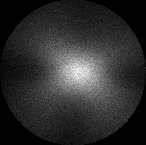
\includegraphics[width=1.0\linewidth, height=7.5cm]{FWF2_5am.jpeg} 
\caption{FW mode no central exclusion}
\label{FW_5am}
\end{subfigure}
\begin{subfigure}{0.48\textwidth}
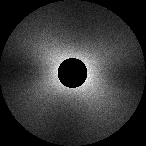
\includegraphics[width=1.0\linewidth, height=7.5cm]{FWF2_5am_1am.jpeg}
\caption{FW mode with $1$ $am$ central exclusion}
\label{FW_5am_1am}
\end{subfigure}
\caption{FW Mode outputs}
\label{FW_op}
\end{figure}
\begin{figure}[h]
\begin{subfigure}{0.32\textwidth}
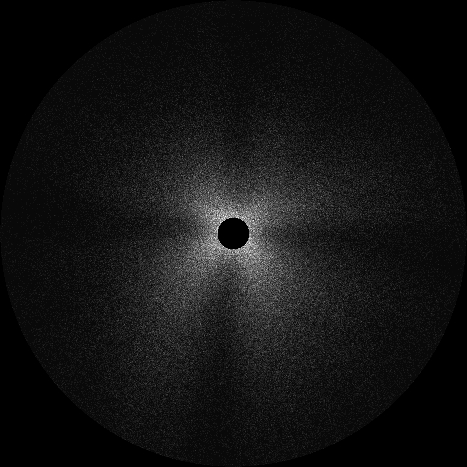
\includegraphics[width=1.0\linewidth, height=5cm]{PCP4_1am.jpeg} 
\caption{PC mode with $1$ $am$ exclusion}
\label{PC_1am}
\end{subfigure}
\begin{subfigure}{0.32\textwidth}
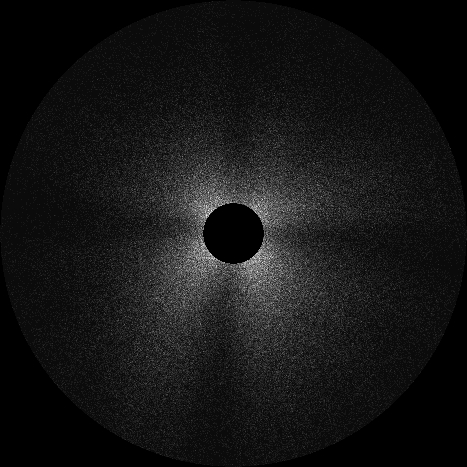
\includegraphics[width=1.0\linewidth, height=5cm]{PCP4_2am.jpeg}
\caption{PC mode with $2$ $am$ exclusion}
\label{PC_2am}
\end{subfigure}
\begin{subfigure}{0.32\textwidth}
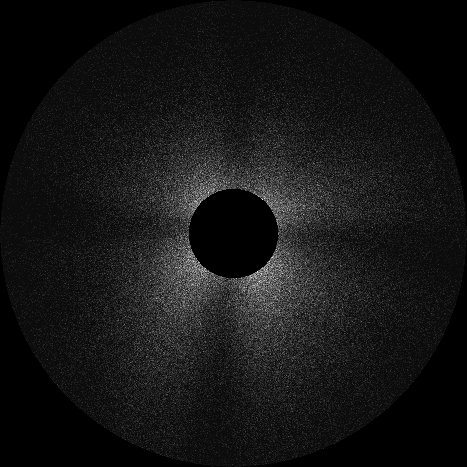
\includegraphics[width=1.0\linewidth, height=5cm]{PCP4_3am.jpeg}
\caption{PC mode with $3$ $am$ exclusion}
\label{PC_3am}
\end{subfigure}
\caption{PC Mode outputs}
\label{PC_op}
\end{figure}
\paragraph{}
Once the region filtering is done, and we have obtained the images as mentioned above, we are supposed to save each outputs with the command:
\begin{center}
\item \large \textbf{save all}
\end{center}
\paragraph{}
The above command will save the light curve as a .lc file, the image as a .img file, the spectrum as a .pha file and the event as a .evt file. 
\paragraph{}
Note that on region filtering and then plotting the image we might not exactly get the same output as shown above, what I have shown in Figure \ref{FW_op} and \ref{PC_op} are what you would see on opening the spectrum file (i.e. the .pha file) in ds$9$. 
\paragraph{}
At this point, the work of Xselect is pretty much done. We would now move on to Xspec. 
\subsection{Step 4: SXTMKARF}
\paragraph{}
When the telescope is collecting data, there is a finite probability that the data that we receive might be off-axis, when compared to the telescope axis, meaning, the peak intensity wont be at the center of the sensor. Now, recall that the effective area, and the quantum efficiency is multiplied together to obtain the Auxiliary Response File (arf). Now, since the quantum efficiency depends on the aspect solution (which in turn means how well the telescope is pointing towards the object and how well it is able to track the object over time), any off centered object (i.e. poor/bad aspect solution) would cause changes in the ultimate result. Hence a tool such as sxtmkarf is used to generate an OGIP style arf which would have its center as the object's center and not the telescope's axis. In FW mode this shouldn't make much difference, however, in PC mode this would make a considerable difference. 
\paragraph{}
Now in order to perform the necessary corrections we use the following inputs:
\begin{enumerate}
\item Spectrum file 
\item ARF 
\item RMF 
\item The RAWX and RAWY coordinates of the center of the object.
\end{enumerate}
\paragraph{}
We have all the data by this point other than the RAWX and RAWY coordinates. In order to obtain that we need to use Xselect and plot the image (with the time filters and without region filters). Once done, the following instruction is used to set the coordinates to RAWX and RAWY coordinates.
\begin{center}
\item \large \textbf{set xyname rawx rawy}
\end{center}
\paragraph{}
Then we need to extract and plot the image. Upon which we would see that on hovering the mouse over the object, instead of seeing its wcs coordinates, we would see the  pixel coordinates. Now, in order to get the centroid coordinates, select a circular region, and place it at the center of the object, roughly. Once done, the information window (the one we used to see the dimensions of the region while region filtering) would show you the centroid coordinates. However, it is crucial that one does not use these centroid coordinates yet. In order to obtain the correct (or close to correct) centroid we would have to click on the region drop down menu from the tool bar and keep clicking on the centroid button, upon doing so, you would observe the region moving. Keep clicking unless the region stops to move. Once done, we now would have a region that is very close to the centroid. Note down the centroid coordinates from the information window. The first coordinate is rawx and the second is rawy. 
\paragraph{}
Once we have this last bit of information, we can proceed with generating an off-axis arf using the SXTMKARF tool. 
\paragraph{}
In order to run this tool, we need the file sxtmkarf.sh, which comes with the software package. In order to run this we first need to "tell" the system to accept and run the python script as a command with access to change files in the working directory. We do that by using the command: 
\begin{center}
\item \large \textbf{chmod 755 sxtmkarf.sh}
\end{center}
\paragraph{}
After which we use the command:
\begin{center}
\item \large \textbf{./sxtmkarf.sh}
\end{center}
\paragraph{}
To compile and run the python script. This instruction then goes into the sxtmkarf.sh text file and based on the parameters mentioned within the file executes the sxtmkarf command with the mentioned parameters as arguments. The text with arguments (in bold) will look something like this:
\paragraph{}
$sxtmkarf$ \\$phafile=(your \ spectral \ file).pha $ \\$outfile=(output \ file \ name).arf$\\ 	$rmffile=(the \ default \ response \ file).rmf$ \\$inarffile=(the \ default \ arf \ file).arf$\\ $expofile=NONE$ \\ $psfflag=N$\\ $vigfile=CALDB$\\$srcx=-1$ \\$srcy=-1$ \\$chatter=4$\\ $clobber=Y$ \\$history=Y$\\ $cphead \ (the \ default \ arf \ file).arf+1 \ (output \ file \ name).arf+1$
\paragraph{}
Note that the user is supposed to copy and paste the names of their respective files in place of the files I have mentioned above as arguments. The last line is crucial as well since this is the instruction that is responsible for copying the headers from the old arf to the new arf, so that xspec is able to recognize the new off-axis arf as a valid input. 
\paragraph{}
Once the user enters all the above, and saves the contents of the file and then runs the execution command, the program should ask for the rawx and rawy coordinates of the centroid, once entered, the program should give you the output with the entered name, besides $outfile$. * Don't forget to initialize heasoft first *
\paragraph{}
Once done, the user should have the required off-axis arf files to work with on the spectrum file which will be explained in the following section.
\newpage
\subsection{Step 5: Xspec}
\paragraph{}
Now that we have extracted the spectrum files we can move on to spectral analysis using Xspec. There are in particular four files we need as inputs for Xspec.
\begin{enumerate}
\item The Spectral file i.e. the pha file
\item The Background pha file
\item The Response file, i.e. the rmf file, and 
\item The Auxiliary response file, i.e. arf file.
\end{enumerate}
\paragraph{}
The \textbf{Spectral File}, as discussed previously, contains the point based count histogram obtained from an X ray observation, representing the integrated charge per pixel from an event. 
\paragraph{}
\begin{wrapfigure}{r}{0.35\textwidth}

\includegraphics[width=1.0\linewidth, height=5cm]{Background_crab.jpeg}
\caption{Detector Background}
\label{Back_sample}
\end{wrapfigure}
Similarly, the \textbf{Background File} contains the background counts observed by the satellite, and looks something like the image shown in figure \ref{Back_sample}. Other than the occasional background flares, the background  soft cosmic x-rays and cosmic ray induced events are relatively constant and do not change much over time (meaning, their behavior is quite predictable), the background pha file doesn't really need any change.
\paragraph{}
The \textbf{Redistribution Matrix File} (rmf) contains the probability map of all the pixels to detect an event when a X ray photon is incident on the sensor. This is sensor dependent and hence remains the same for a particular sensor. In other words, rmf maps the energy space into detector pulse height (or position) space. An ARF (Auxiliary Response File) is needed with an RMF to produce the input energy spectrum  weighted by telescope area and detector efficiencies. (**)
\paragraph{}
The \textbf{Auxiliary Response File} (or arf) contains the combined telescope/detector/filter effective areas (because of reflectivity and vignetting and other such effects, the geometric area of the telescope is reduced to an effective area), and the quantum efficiency of the detector as a function of energy averaged over time (and therefore over aspect solution). This means that a bad aspect solution data would give skewed values. Hence it is necessary for us to use tools like SXTMKARF in order to correct for this error, by generating arf files which are off-axis (to match up with the bad aspect data) using the pha files from the data we extracted from Xselect. 
\paragraph{}
Based on the aforementioned discussion on the types of files needed for Xspec to work; Xspec uses those files as follows:
\begin{enumerate}
\item Choose a parameterized model which is thought to represent the actual spectrum of the source.
\item Choose values for the model parameters. 
\item Based on the parameter values given, predict the count spectrum that would be detected by the spectrometer in a given channel for such a model.
\item Compare the predicted spectrum to the spectrum actually obtained by the instrument.
\item Manipulate the values of the parameters of the model until the best fit between the theoretical model and the observed data is found.
\item Then calculate the “goodness” of the fit to determine how well the model explains the observed data, and calculate the confidence intervals for the model’s parameters.
\end{enumerate}
\paragraph{C(I): The Observed Spectrum}
In order to generate an observed spectrum, Xspec uses two files, The input pha file (or in better terms the data file) containing D(I), and the background file containing B(I), both being a function of the energy channel I. The data file tells Xspec how many data counts was detected by the instrument in a given channel and the background file tells the same for background photons in a given channel. Xspec then uses the back file to obtain a set of background subtracted spectra C(I) in units of counts per second. The background subtracted count rate (for each spectrum) is given by (ref. Xselect manual);
\begin{equation}
{C(I)} = \frac{D(I)}{a_{D(I)} t_D} - \frac{b_{D(I)}}{b_{B(I)}} \frac{B(I)}{a_{b(i)} t_B}
\end{equation}
\paragraph{}
where D(I) and B(I) are counts in data and background files, ${t_D}$ and ${t_B}$ are exposure times in the data and background files, ${b_{D(I)}}$ and ${b_{B(I)}}$ are background scaling values from data and background files and ${a_{D(I)}}$ and ${a_{B(I)}}$  are area scaling values from data and background files, which together refer the background flux to the same area of the observation as necessary. When this is done, Xspec has an observed spectrum to which the model spectrum can be fit.
\paragraph{R(I,E): The Instrumental Response}
Before Xspec can perform any prediction, Xspec must know the specific characteristics of the instrument. This information is known as the detector response. Recall that for each spectrum the response R(I, E) is proportional to the probability that an incoming photon of energy E will be detected in channel I. As such, the response is a continuous function of E. This continuous function is converted to a discrete function by creating a response matrix which defines the energy ranges $E_j$ such that (ref. Xselect manual):
\begin{equation}
{R_D(I,J)} = \frac{\int\limits_{E_{J-1}}^{E_J} R(I,E) dE}{{E_J}-{E_{J-1}}}
\end{equation}
Xspec reads both energy ranges $E_J$ and the response matrix $R_D (I,J)$ from a response file in a compressed format that only stores non zero elements. 
\paragraph{}
XSPEC also includes an option to use an auxiliary response file, which contains an array $A_D (J)$ that is multiplied into $R_D (I, J)$ as follows (ref. Xselect manual *Insert Xselect manual reference here*):
\begin{equation}
{R_D (I,J) \rightarrow R_D (I,J) \times A_D (J)}
\end{equation}
\paragraph{}
This array is designed to represent the efficiency of the detector with the response file representing a normalized Redistribution Matrix Function, or RMF.
Conventionally, the response is in units of $cm^2$.
\paragraph{M(E): The Model Spectrum}
The model spectrum, M(E), is calculated within XSPEC using the energy ranges defined by the response file (ref. Xselect manual):
\begin{equation}
{M_D (J) = \int\limits_{E_{J-1}}^{E_J} M(E) dE}
\end{equation}
and is in units of photons/$cm^2$ /s. XSpec allows the construction of composite models consisting of additive components representing X-ray sources (e.g.,power-laws, blackbodies, and so forth), multiplicative components, which modify additive components by an energy-dependent factor (e.g., photoelectric absorption, edges, ...). Convolution and mixing models can then perform sophisticated operations on the result. Models are defined in algebraic notation.
\paragraph{Fits and Confidence Intervals}
Once data has been read in and a model defined, XSpec uses a fitting algorithm to find the best-fit values of the model parameter. At the end of a fit, XSpec will write out the best-fit parameter values, along with estimated confidence intervals. These are one sigma confidence intervals and are calculated from the second derivatives of the fit statistic w.r.t. the model parameters at the best-fit. These are however unreliable. XSpec has a separate command (error or uncertain) to derive confidence intervals for one interesting parameter, which it does by fixing the parameter of interest at a particular value and fitting for all the other parameters. New values of the parameter of interest are chosen until the appropriate delta-statistic value is obtained. XSpec uses a bracketing algorithm followed by an iterative cubic interpolation to find the parameter value at each end of the confidence interval.
\paragraph{}
Now that we have had a basic idea as to what XSpec does with the data, let us see how the operations are realized in practice using commands. 
\paragraph{}
We first start by initializing HEASoft (as we do for Xselect) and then we initialize XSpec. Once done, we should see the XSpec prompt like this:
\begin{center}
\item \large \textbf{XSPEC12$>$}
\end{center}
\paragraph{}
We then enter the following commands in sequence to initialize XSpec with the data. 
\begin{center}
\item \large \textbf{XSPEC12$>$ data (data file name with location and extension)}
\item \large \textbf{XSPEC12$>$ back (back file name with location and extension)}
\item \large \textbf{XSPEC12$>$ resp (rmf file name with location and extension)}
\item \large \textbf{XSPEC12$>$ arf (arf file name with location and extension)}
\end{center}
\paragraph{}
To check whether the data is initialized correctly, we type the following command:
\begin{center}
\item \large \textbf{XSPEC12$>$ show data}
\end{center}
\paragraph{}
If we get an output as follows; then we know that the data has been accepted by Xspec.
\begin{figure}[h]
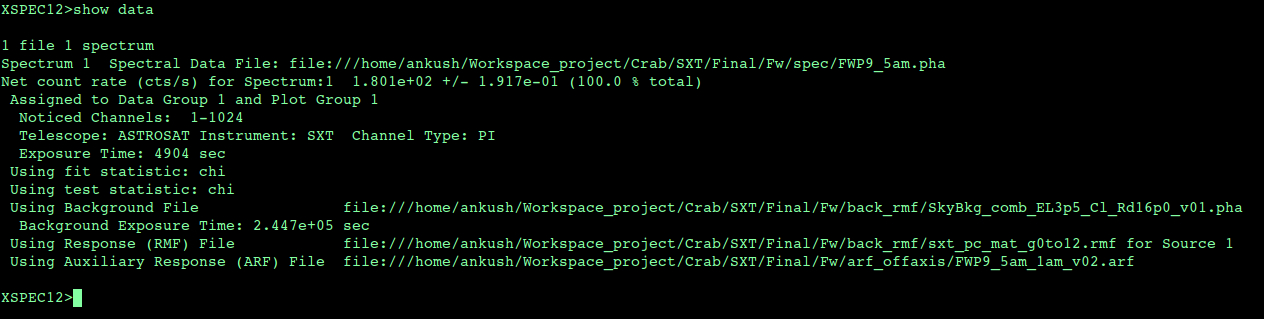
\includegraphics[width=1.0\linewidth, height=5cm]{xspec_sd.jpg}
\caption{Xspec show data output}
\label{Xspec_show_data}
\end{figure}
\paragraph{}
We now need to set the plot to an energy scale so that we get the normalized count (i.e. counts compared to the reference level set by the rmf and arf files) with energy in KeV. This is done by using the command:
\begin{center}
\item \large \textbf{XSPEC12$>$ setplot energy}
\end{center}
\paragraph{}
Now, since the energy sensitivity range of SXT is $0.3$ to $8.0$ $KeV$, anything other than that would be meaningless data. However, the signal to noise ratio towards the ends of the energy range is high, hence it is advisable that we consider only the central region of the spectrum (Note that you can use this command to ignore channels as well, just don't enter the channel limits in float, because for this command, float=energy in KeV, and integer=channel number). We do the above using the following command:
\begin{center}
\item \large \textbf{XSPEC12$>$ ig **-0.7 7.0-**}
\end{center}
\paragraph{}
Here, ig is a short form for ignore. The above command tells xspec to ignore all the energies below $0.7$ $KeV$ and above $7.0$ $KeV$. One thing that helps us mediate the binning issues is \textbf{grppha} to bin the data, which would help reduce the impact due to noise, among several other things (ref. *insert xspec manual reference here*) on the model fit and hence it's impact on the reduced $\chi^2$ value.
\paragraph{}
Now, we are ready to introduce a simulation model into xspec. As mentioned above, we do that by using the model (or mo, in short) command as follows;
\begin{center}
\item \large \textbf{XSPEC12$>$ model tbabs*(powerlaw)}
\item \large \textbf{1:TBabs:nH$>$ $0.21$}
\item \large \textbf{2:powerlaw:PhoIndex$>$ $2.14$}
\item \large \textbf{3:powerlaw:norm$>$ $10.4$}
\end{center}
\paragraph{}
We can also enter the command mo tbabs*(po) in place of the above since both mean the same. Now, as it is mentioned above, we need to take care about the object's location, and basic optical signatures as well in order to conclude what would be a good model for it. Now, in this case since crab nebula is near the galactic arm, the light coming for there would face extinction due to the ISM in the galactic arm. This model calculates the cross section for X-ray absorption by the ISM as the sum of the cross sections for X-ray absorption due to the gas-phase ISM, the grain-phase ISM, and the molecules in the ISM (ref. ). The parameters entered is the best fit parameters that were found out for the ideal case, which is obtained from different sources. 
\paragraph{}
Now, if you wish to change the value of any of the parameters, you do it by using the following command (in this example we are setting the first parameter):
\begin{center}
\item \large \textbf{XSPEC12$>$ newpar *}
\end{center}
\paragraph{}
Now, the format for changing any parameter is as follows:
\begin{center}
\item \large (Value of new parameter) (step value) (minimum limit) ( minimum value) (maximum value) (maximum limit)
\end{center}
\paragraph{}
Once we do that, Xspec asks us for parameter values for nH, phoIndex and Norm, however, for now let us exit the terminal using /*. Once done, we now command xspec to fit the predicted model to the data received, using the command;
\begin{center}
\item \large \textbf{XSPEC12$>$ fit}
\end{center}
\paragraph{}
Once done, Xspec fits the model spectrum to the data spectrum. And Xspec writes down the best fit parameter values. Now, we would have to plot the spectrum with our plotting tool. The one I used was xw. To load the tool we need to type the following command; 
\begin{center}
\item \large \textbf{XSPEC12$>$ cpd /xw}
\item \large \textbf{XSPEC12$>$ pl ldata ratio}
\end{center}
\paragraph{}
The above command plots the logarithmic data on both axes. It also plots the variations in the data when compared to our model in a graph below the plot. The output is as follows;
\begin{figure}[h]
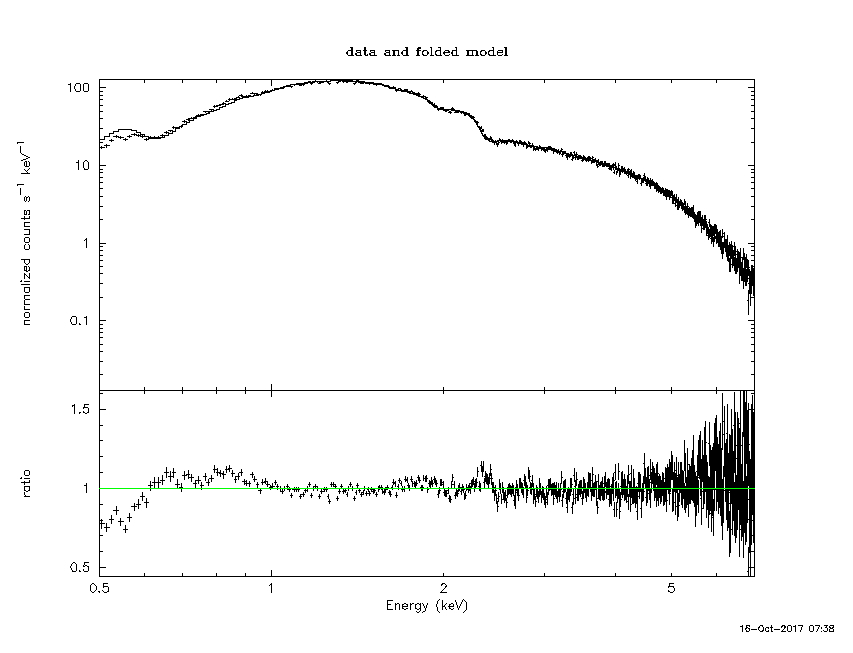
\includegraphics[width=1.0\linewidth, height=10.5cm]{7.jpg}
\caption{log data plot}
\label{log_dp}
\end{figure}
\paragraph{}
The next thing we would have to do after we plot is to adjust the gain of the model. This is done using the command; 
\begin{center}
\item \large \textbf{XSPEC12$>$ gain fit}
\item \large \textbf{slope$>$ $1$ $-1$}
\item \large \textbf{offset$>$   }
\item \large \textbf{XSPEC12$>$ fit}
\end{center}
\paragraph{}
This would adjust the gain so that we have a slope frozen to 1 and an offset calculated by the system, to have the best fit. We then fit the above and use the command \textbf{pl} again to obtain the above plot (Figure \ref{log_dp}). 
\paragraph{}
Now, we can see that the low energy region shows a significant amount of deviation. This can be further corrected using several commands, one of them being setting the solar abundances using the command, abund. As a rule of thumb, it is our intention that the normalization be the lowest possible. And, the $\chi ^2$ value be close to one. Now, there are several tables used for plasma emission and photoelectric absorption models. We could set different abundances, however, the table ``wilm" seems to give us the least norm and $\chi ^2$ value closest to one. So we would follow this abundance model for now. We do that by using the following command:
\begin{center}
\item \large \textbf{XSPEC12$>$ abund wilm}
\item \large \textbf{XSPEC12$>$ fit}
\end{center}
\paragraph{}
After that we get the following curve:
\begin{figure}[h]
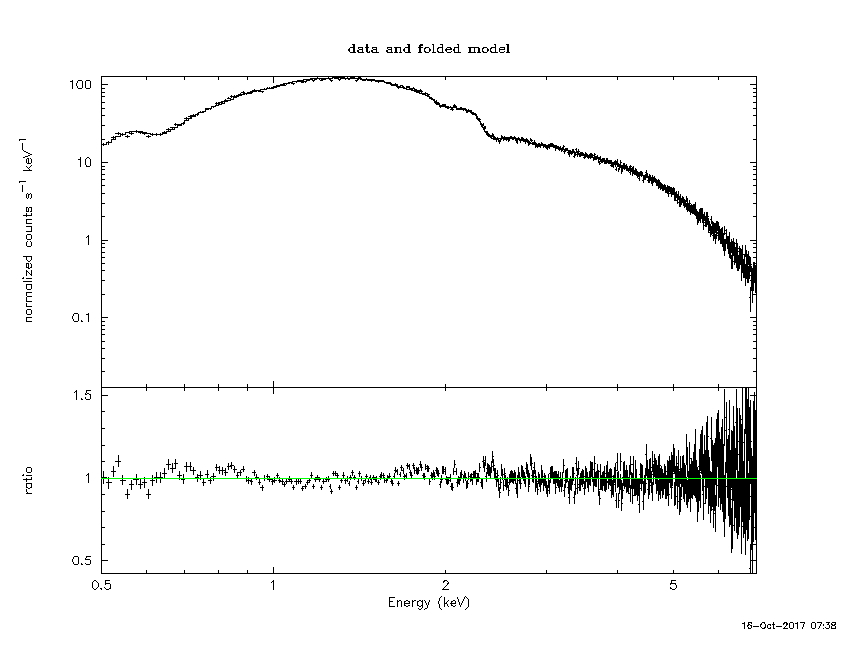
\includegraphics[width=1.0\linewidth, height=10.5cm]{8.jpg}
\caption{log data plot with abundance set with wilm table}
\label{log_dp_abund}
\end{figure}
\paragraph{}
However, it is not mandatory that we stick to one model since it depends on the source as to what solar abundance ratio table is appropriate for it, hence, we might do well to check other abundance models as well. I say this because different elements form by different processes. Some of the elements are formed by type II supernovae (light metals i.e. Mg, C, O etc. Note that anything heavier than Hydrogen and Helium is considered a metal) and some are formed by type Ia supernovae (i.e. the ``Iron peak" elements i.e. Fe, Ni, Zn, Co, Mn, Cr). Type II supernovae are  mostly because of massive stars (meaning, stars with low life time, since they are burning fuel, faster) and type Ia supernovae are because of white dwarf stars exploding in a binary system when they go over the Chandrasekhar limit, maybe due to in-falling matter from the companion star (in short they are from stars that have had a long life span, i.e. low to intermediate mass star). Since these stars go ``boom" at different times, the elements formed by these explosions are incorporated into new stars at different epochs during the star formation history of the galaxy. This could mean, that finding a correct (that gives $\chi ^2 \approx 1$ meaning an ideal fit of our model with the data) solar abundance model (comparison of log of element to element ratio in the observed object to that of the same element to element ratio in the sun) could give us an idea as to what that source is made up of. However, this hypothesis is up for debate because of my lack of knowledge, as of now. Also, looking at the abundance ratio of different stars can give us strong clues as to what their age might be.
\paragraph{}
Since the object we are observing also happens to be an emission nebula, there are certain photoionisation effects that could impact our data since the model we are using is an absorption model. We do that by using the command, xsect. Now, there are three options in this case;
\begin{enumerate}
\item obcm (from Balucinska-Church and McCammon with old Helium crossection), 
\item bcmc (from Balucinska-Church and McCammon with new Helium crossection), and,
\item vern (from Verneret. et. al.)
\end{enumerate}
\paragraph{}
For now, we will be using bcmc. We do that as follows:
\begin{center}
\item \large \textbf{XSPEC12$>$ xsect bcmc}
\item \large \textbf{XSPEC12$>$ fit}
\end{center}
\paragraph{}
The last thing that we need to define is the systematic error in the model we used. We do that with the help of the command systematic. Systematic errors are the errors that might be introduced into the final result due to flaws in the equipment or in the design of the experiment. Unlike random errors, systematic errors cannot be reduced by merely repeating the experiments with the same equipments, and hence may lead to an overall alteration of the final result. Hence there is a need to introduce a model dependent systematic term to the variance. We set a systematic error of $2$\% by using the following command. 
\begin{center}
\item \large \textbf{XSPEC12$>$ systematic $0.02$}
\item \large \textbf{XSPEC12$>$ fit}
\end{center}
\paragraph{}
Once we reach this step, we now have the results of the object in que
\;stion which we need to analyze. We also have the final plot of the en[-ergyp] spectrum by now. Note that since the properties of every object are different, the above method (which was for the crab nebula data that I had) will vary. A significant variation will be with the model we would use, which, as mentioned above is completely based on the object we are observing and it's property. In case of this being an unknown source, we are supposed to take educated guesses as to what the object might be like, hypothesize, accordingly select the model, look at the reduced $\chi ^2$ value and judge whether the model we used to fit is the correct model explaining the source. If not, then rinse and repeat unless we find the best fit model. As mentioned in the previous sections, we check for the goodness of the output by using two commands;
\begin{center}
\item \large \textbf{XSPEC12$>$ goodness}
\item \large \textbf{XSPEC12$>$ error 1-3}
\end{center}
\paragraph{}
These commands help us determine whether the variation in values we got for the three parameters (if we use one model to fit), i.e. nH, phoIndex and norm, has the accepted values of those parameters within their variation range. If not, then we are making some mistake somewhere. 
\paragraph{}
Note that this command is crucial for you to determine whether the fit is proper or not. The error command would refit the entire spectrum again and again unless the model fits the data properly. 
\newpage
\section{LAXPC data processing}
\paragraph{}
Now, once the software is set up, which is mentioned in the previous section, we will perform the following steps to obtain the data required to plot the light curves and spectra. Now, since it is mentioned that there are two software for LAXPC data processing, we would stick to one software package for analyzing the data. Now, another thing to note is that the pipeline from IUCAA, had some problems with processing the background files, at the time of writing this report, I am not sure whether this is resolved yet, however, because of this, we would be sticking to the code by Dr. H. M. Antia, with the new background software (released in December $2017$). Also, since I mentioned that the IUCAA code is just with a python shell around the FORTRAN code by Dr. Antia, I would  focus on how to use the code from Dr. Antia, for now. 
\paragraph{}
Unlike the SXT analysis, the number of steps needed to analyze the LAXPC data is comparatively less since most of the work is done by a black box pipeline software (reason being I myself am not sure how the software works =]exactly). Things such as the GTI filtration is done by the software and we need not bother with explicitly removing the GTI like we did during SXT analysis. Now, one of the primary differences in a proportional counter design and a telescope design is the fact that telescope focuses the photons, and the proportional counter counts the energy of the photons based on how far they go within the Xenon-methane gas, i.e. based on what anode layer depth they go. 
\paragraph{}
Now, why is LAXPC used? Other than the fact that the energy range is broad (at the time of writing this report, LAXPC has the largest sensitivity range possible for any X-ray Proportional Counter, which is $3-80$ $KeV$ energy range), one of the many uses being the data generated is perfect for power spectrum analysis, i.e. plotting the power spectrum using the data, because the Nyquist frequency achievable using the data obtained goes upto $4000$ $hz$ and above if I recall correctly. This helps us detect QPOs, thermonuclear bursts (not sure if they would show up in frequency powspec), and other such signatures. 
\paragraph{}
Now, the software is responsible to convert the level one data into level two. This is unlike the data that is processed in SXT since the data we work with is level $2$ data. The LAXPC software corrects for the GTI (poor aspect solution, high background e.t.c.), and other such effects. Once done, the software generates the light curve and the background light curve out of this data which is then used with the software such as lcurve (to obtain light curve) or powsepc (to obtain the power spectrum) out of the data. 
\subsection{Processing steps}
\paragraph{}
Once the data is obtained, it should be in the following format. 
\begin{figure}[h]
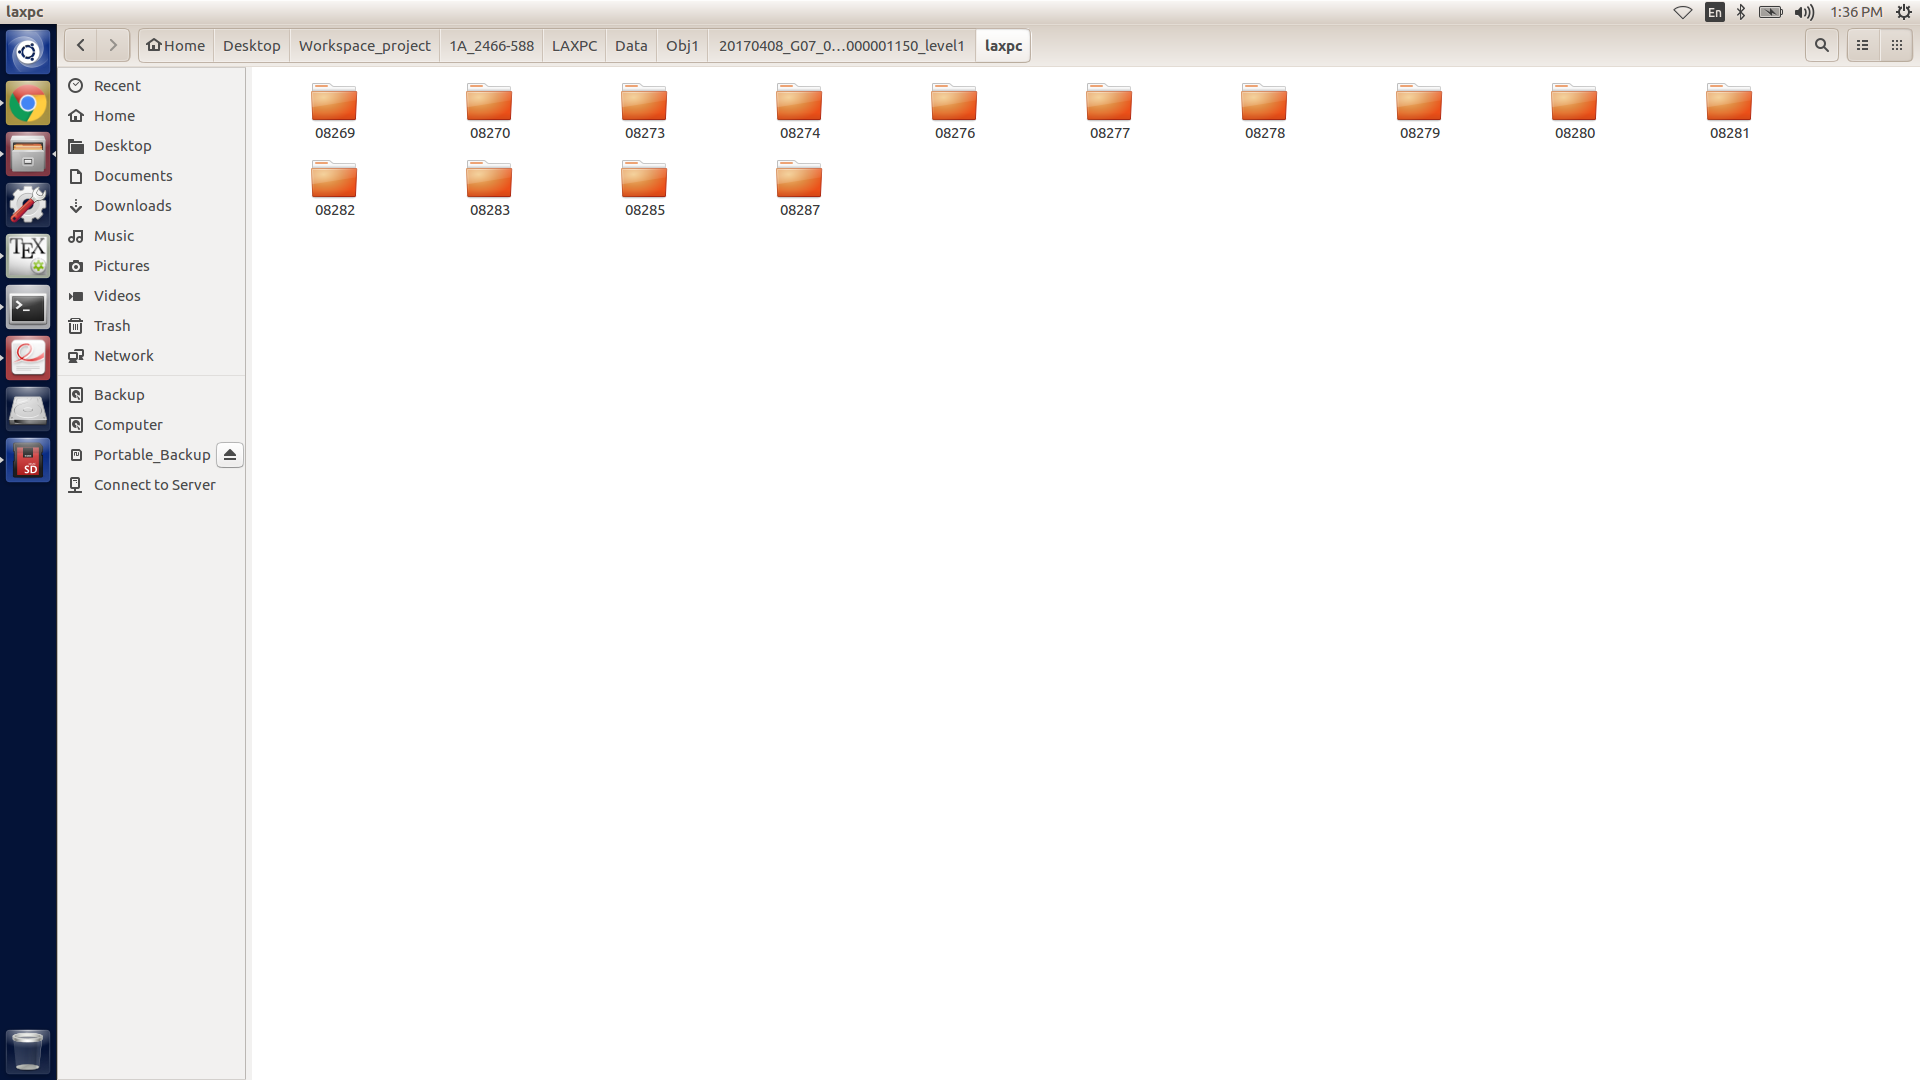
\includegraphics[width=1.0\linewidth, height=8cm]{Screenshot_from_018-02-03_13-36-32.png}
\caption{LAXPC data sample}
\label{LAXPC_data_sample}
\end{figure}
\paragraph{}
Now, in the above image, each file represents one orbit, where the GTI isn't filtered. Now, the data wouldn't always be in the same format as shown, since it depends on how the data was obtained. Now, the main intension of the user would be to obtain the data in the form as shown above, i.e. all the orbits in the same directory as shown. One way to do that would be to use the copy command from linux to copy all of them in one directory.
\paragraph{}
Now, once done, we are ready to work with the data. We now have to make a list of four particular files within each orbit. It is in a format as shown below:
\begin{center}
\item {$20170408\_G07\_065T02\_9000001150\_level1/laxpc/08269/AS1G07\_065T02\_9000001150lxp\_level1.mkf$}
\item {$laxpc/08269/aux/AS1G07\_065T02\_9000001150lxp\_level1.tct$}
\item {$laxpc/08269/lxp1/modeBB/AS1G07\_065T02\_9000001150lxp1BB\_level1.fits$}
\item {$laxpc/08269/lxp1/modeEA/AS1G07\_065T02\_9000001150lxp1EA\_level1.fits$}
\end{center}
\paragraph{}
The main goal now is to make a list of these files, i.e. the two .fits, one mkf and one .tct file from every orbit into one list file having the locations of the said files. laxpcl1, i.e. the fortran executable file requires these files to run. There is a script written to perform this function, with the name \textbf{findfile}. One would have to change the arguments in this file and run this file. You would have to change the location within the file for it to work. It is just a script that finds files within any directory and procedurally copies the locations of these files into one file. The output file would be called ls1 (the name can also be changed within the find file script). 
\paragraph{}
Another thing to note is that for laxpcl1 to work, one would need a gti interval as well. This is not present by default, and hence each time you wish to run the laxpcl1 script, it would look for the good time interval file, and hence would give an error prompt if it does not find the file. Hence one would have to first create a file \textbf{gti.inp} and in the first line put $0$. This is done so that the software can detect a blank file which it will later change and put in the correct gti intervals. 
\paragraph{}
Once these things are done, one can run the laxpcl1 script. In the first line it would ask you for the pcu number, i.e. out of the $3$ LAXPC pcu, which one would you like to use. Note that at the time of writing this report, the $3^{rd}$ pcu is not operational, since there is some kind of leakage in the chamber, because of which the pressure in the pcu isn't exactly 2 atmospheres, and hence it's composition is different from the other pcus, hence rending the data un-reliable. 
\paragraph{}
However the next thing which the program will ask for is the time bin needed. This is where you define the time bin needed by you. Note that this is also important since this decides the Nyquist frequency (half of max sampling frequency, needed in power spectrum). For example, if you would want to detect some event that you hypothesize to give a peak frequency of $300$ $Hz$, then you need to have a time bin of less than 0.006 seconds. This would translate to the maximum possible frequency of $300$ $Hz$, (insert van der klis paper reference). After that we mention the anode layers we need, \textbf{0} for all the layers, \textbf{1} for the top layer (A1+A2), \textbf{3} for Second layer (A3+A4), \textbf{2, 4 to 10} for the respective anode layers. For example, to get the laxpc pcu $1$ data, for a time bin of $0.00025$ seconds (Nyquist frequency of $2000$) and the data from all the pcu levels, we enter the following;
\begin{center}
\textbf{1 0.00025 0}
\end{center}
\paragraph{}
Then, the software will prompt for the channel numbers needed, i.e. the lower channel limit and the upper channel limit, the signal within which will be considered. The rest of the signal, outside these channel numbers will be ignored. Now, in order to find out the channel number, and their corresponding energy ranges, we need to open the response file for the particular pcu at the time of the observation. This is done using the software called backshiftv2 which is generated along with laxpcl1 (but using a different FORTRAN code). Now, once you execute the executable file, (similar to laxpcl1), it will ask for the pcu number and the and the anode level, the anode labeling is same as the one used for ./laxpcl1 in the previous paragraph. Then once you press enter it should ask for the time bin, lower limit channel number, upper limit channel number, and nul flag, which is a flag to fit low energy background. set it to $-2$ for using fit to layer 1 background for channels 0-200 (< about $20$ $keV$). Now, since you do not have any output from ./laxpcl1 yet, you will not have the file it asks for next, which is the background file generated from ./laxpcl1. However, keep the section blank and just press enter. Upon doing so, the software would give you an error and would prompt you to enter the date of the observation, upon doing so, and pressing enter, look for a line that says, "\textbf{use ---- response file}", note down the name of that response file. Now, assuming you have downloaded the latest response files from the website, you would have to find the response file within that folder containing responses for every consecutive dates, and once found, open that response file with fits viewer (part of heasoft package, hence you would have to initialize heasoft first, and then enter fv followed by the fits file name). Once open, look for the \textbf{EBOUNDS} row, and under the view column, click on 'All', this will display the energy bounds for the respective channels. Write down the channel numbers for the respective energy bounds. This is what enter as the lower and upper channel limit. 
\paragraph{}
Once done, the software will ask for the number of channels to be used in the spectrum. The response files are made with $512$ channels for LAXPC PCU $1$ and $3$, and $256$ channels for LAXPC PCU $2$. This could also be seen when one opens the response files for each pcu (found out using the backshiftv2, for each pcu). 
\paragraph{}
Once done, the software should ask for earth occultation correction, this is done because, as mentioned in the previous section, ASTROSAT takes data throughout the orbit, even while it is behind earth when facing the object, LAXPC has a provision of correcting this, hence this step. For starters, unless mentioned, we will consider skip this step with \textbf{*/}, and press enter. 
\subsection{Products}
\paragraph{}
After doing that, the software will process and finally through out the following data:
\begin{enumerate}
\item \textbf{lxpilevel2.event:} Summary of frames read from level 1 EA mode, the 'i' in the file name stands for i$^th$ pcu. So, for LAXPC1, it would be lxp1level2.event
\item \textbf{lxpilevel2.evn:} This is the FITS giving data for each "valid" event. The quotations around valid is to emphasize when a GTI interval is considered, i.e. refer the part where we discussed what makes a GTI.
\item \textbf{lxpilevel2.evn1:} This the ASCII file containing the event data.
\item {\textbf{lxpilevel2.lc:} This is the ASCII file for the light curve. The following are the column value (ref. the manual attached within the laxpc folder):
\begin{enumerate}
\item \textbf{col-1:} Instrument time (sec from switch on of STBG)
\item \textbf{col-2:} UTC time (sec from 1 Jan 2010)
\item \textbf{col-3:} counts in the specified time bin (\textbf{not count rate})
\item \textbf{col-4,5:} RA, Dec of pointing direction (in deg)
\item \textbf{col-6-8:} Longitude, latitude (in deg) and altitude (km) of satellite
\item \textbf{col-9:} Elevation of source above the Earth's limb (in deg)
\item \textbf{col-10:} ULD count rate (per sec)
\item \textbf{col-11:} CPM counts
\item \textbf{col-12:} Fitted background count rate (per sec)
\item \textbf{col-13:} Rate of rejected events (per sec)
\item \textbf{col-14:} Total count rate in all anodes and channels corrected for dead-time.
\end{enumerate}
There are other entries in the file as well in the last line of the document, they are (from left):
\begin{enumerate}
\item ObsID of the last file processed along with source and observer names
\item lxpi: giving the detector used
\item frbk: A factor by which the fitted background in the 12th column of the file needs to be multiplied if range of anodes or channels is restricted.
\item Efficiency of observations, i.e., fraction of GTI during the entire observation
\item fbk: A factor by which the average background spectrum is multiplied, depending on the latitude and longitude range covered during observation
\item fraction of time in data gap (excluding SAA)
\item Total exposure time for observation in sec as obtained from GTI
\item Fraction of frames lost, i.e., missing or marked bad or eliminated
\end{enumerate}
}
\item \textbf{lxpilevel2.lcurv:} FITS file giving the light curve. This shows only the time covered by GTI and shows count rate per sec. The count rate is for the specified anode and channel range and is corrected for the dead-time.
\item \textbf{lxpilevel2.lcbk:} FITS file giving the light curve for fitted background model. This shows the time covered by GTI and the count rate per second. The cont rate is for a specified anode and channel range and is corrected for the dead time. 
\item \textbf{lxpilevel2.pha:} ASCII file giving the spectrum. It contains count rate per sec averaged over all time specified by GTI. The number of channels is taken from the input value for NCA. First column is channel number, the next 10 columns are count rate in anodes A$1$-$10$ and last column is the total count rate in A$1$-$7$. Irrespective of value of input parameter IAN all anodes are included. The spectrum is corrected for the dead-time.
\item \textbf{lxpilevel2.spec:} FITS file giving the spectrum for the specified anode averaged over all time specified by GTI.  The number of channels is taken from the input value for NCA. The spectrum is corrected for the dead-time.
\item \textbf{lxpilevel2back.pha:} ASCII file giving the modelled spectrum for the background averaged over the same duration as the source spectrum. For NUL=0 the background model based on ULD counts is used, while for NUL=$-1$ background model based on fit to latitude and longitude is used.  For NUL=$-3$ fit in 3D is used, but this is not very good. The format is the same as that for source spectrum.
\item \textbf{lxpilevel2back.spec:} FITS file for background spectra for the specified anode. The format is the same as that for source spectrum.
\item \textbf{lxpilevel2.gti:} ASCII file giving the GTI generated from the observed light curve.  The first line is no. of entries and the subsequent lines specify the time range. First two columns specify the Instrument time which are used by the program, the next two columns are in UTC. This file can be edited and moved to gti.inp and the program has to be run second time to use the GTI input. To generate GTI file it is advisable to run the program with a time bin of about 1 sec and full range of anodes and channels. Once the gti.inp file is prepared the program can be run for required time bin, anodes and channels.
\item \textbf{lxpilevel2.four:} The Fourier transform of the entire light curve. If there are too many entries then time range  may be truncated. This may not be very useful as it would cover the Earth occultation and SAA passage also, with gaps set to $0$.
\item \textbf{lxpilevel2.mkf:} Summary of .mkf file read. It could be used to check the time range covered by each file or to check if all files are read.
\item \textbf{lxpilevel2.uld:} ASCII file giving the ULD counts as read from the level-1 BBC file.
\item \textbf{lxpilevel2.gap:} The first several lines are same as the .lc file but covering those period when there is a gap in data. The gaps due to SAA passage are excluded. This can be used to identify where data are missing. The last few lines give the range of Instrument time for the gaps and the last line gives the total time lost.
\item \textbf{lxpilevel2.frame:} Summary of frames read from level1 fits files grep Frame lxp?level2.frame will give the summary of frame lost in each orbit one per line giving lxpi, obsID, orbit no., total No. of frames, bad frame, total frames eliminated.
\end{enumerate}
\paragraph{}
As one might notice, the above points have been quoted directly from the read me files provided with the software. One would do good to refer to those if one would like to get an in-depth understanding of the software. 
\paragraph{}
Now that the above is done, we can do several things with the fits files that are provided to us, such as plotting the light curve, and hence obtaining the power spectrum of the same. Now, there are several ways of doing the above, one could use the ASCII files to obtain obtain the plots, I personally used python to plot the data and perform normalizations (Leahy with Poisson noise level = $2$, Fractional rms squared normalization with Poisson noise level = $2$/\textit{meanrate} and  Absolute rms squared normalization with Poisson noise level = $2$ $\times$ \textit{meanrate}). However, at the time of writing this email, I am also working on recreating those plots on IDL and read from the event file, if that would make any difference. 
\subsection{Creating window files using xronwin}
\paragraph{}
Before we go into making the power spectra, we need to know how to filter out outliers in the data and/or remove bad GTIs (Like we did in the case of SXT previously). One of the ways of doing so is to manually point the data using a cursor and remove those time intervals, another way of doing so is to ignore those parts of the data using windows files (this is where the xronwin tool from heasoft comes in). There are four kinds of windows that one can create using xronwin, namely:
\begin{enumerate}
    \item \textbf{Time Windows}
    \item \textbf{Phase Windows}
    \item \textbf{Intensity Windows}
    \item \textbf{Exposure Windows}
\end{enumerate}
\paragraph{}
For our case we would be primarily using time and intensity windows, however, in order to do phase resolved spectroscopy, one might have to use phase windows as well. A detailed description of the different windows can be found at \cite{xronwin1}. Creating a time window lets you filter out unwanted orbits, without having to filter them each time yo create a new light curve. Of-course one can remove the data files of those orbits completely, however, I feel that would actually result in the loss of valuable data, just because there was one outlier in the GTI. 
\paragraph{}
Using xronwin to create time windows is fairly straightforward. Select the time window option, then it would ask if you need to add more time intervals or delete any existing time interval. Select add time interval, and then it would ask for a minimum time and a maximum time. These are to be entered in a specific format as it would be mentioned over there itself. To get the time which needs to be entered, one would have to first open the light curve using lcurve. Then use a limited number of newbins per interval so that one can obtain the start and stop time in MET (Mission Elapsed Time) as would be mentioned in the start and stop time at the bottom of the light curve, and then use that time accordingly to obtain the necessary time interval for the window file. Another, much easier way of doing the same would be to use the GTI file, which gives the GTIs in terms of MJD, and write a program to convert it into MET, which one can then use to create an xronwin time window file. 
\paragraph{}
Apart from creating a time window file, one can, within the same instance, create other windows as well. Just like time windows, intensity windows also share the same logic, wherein, all you need to do is mention the maximum/minimum intensity the light curve will have, which would then create the window file accordingly. 
\paragraph{}
Yes, one can obviously use the ASCII output from the pipeline tools to obtain the lightcurve, and use python to correct for the data gaps and hence plot the power spectrum using python's FFT module (or simply use a tool called stingray which has inbuilt modules to perform FFT and normalize the PS accordingly) or one can use xronwin to get rid of the data gaps by ignoring those time windows, it is heavily dependent on the user and what he/she is comfortable with. 
\subsection{Power Spectrum}
\paragraph{}
The importance of plotting the power spectrum is something of a necessity since knowing what periodicities we have in the signal is something that would tell us a lot of things. Depending on what you are observing, it could be anything, orbit of the satellite around earth, if the object has a companion, then their orbit around each other, if the star is accreting, then the rotation of the disc, so on and so forth. Now, if one wishes to quickly see whether there is anything in the data or not, (which would include red noise and QPOs, etc.) one can simply use the lxpilevel2.four file, which is, as mentioned above, the Fourier transformed power spectrum, i.e. the ASCII file for the power spectrum (since you need FFT to obtain the power spectrum from the light curve). One can simply use tools of their choice to plot the power spectrum, i.e. gnuplot, or fplot (which is a part of the heasoft package), or simply python, which would give you a rough idea if there is anything in the data to spend more time into and look at later. 
\paragraph{}
Now, if the object looks interesting, then one can proceed further to use tools such as powspec, or python to further perform normalizations and hence obtain the plots needed. 
\paragraph{}
If one wishes to perform normalizations using python, one can search for the stingray package for python, and how to use it. One can easily obtain the said normalizations, and other things such as the dynamic spectrum, etc. using the software. 
\paragraph{}
However, since the standard software used to plot power spectrum is called \textbf{Powspec}, I would focus on how can one use it to perform normalizations. Note that powspec, at the time of writing this report just had two normalizations available, i.e. Leahy normalization and RMS squared normalization. Now, when you are using POWSPEC you need to remember that it works with arguments, and hence depends heavily on what parameters you pass it while you execute the "powspec" command. A detailed description of the powspec commands could be found on the powspec.txt available on-line. However, lets say someone wishes to use it, one would need the following: 
\begin{enumerate}
\item The light curve fits file. 
\item The window file (one can use - i.e. the default window file, or generate custom window using xronwin task)
\end{enumerate}
\paragraph{}
Once done, you enter the following in your terminal, ( preferably within your working directory):
\begin{center}
\textbf{powspec norm=.....}
\end{center}
\paragraph{}
In place of the dots (.....) you can have the following options based on what kind of normalizations you need: (ref. powspec.txt found in the ftools page)
\begin{enumerate}
\item \textbf{0} = power spectra is normalized by dividing by the number of good newbins per interval.
\item \textbf{1 or -1} = (d/f); power spectra are normalized such that the (white) noise level expected from the data errors corresponds to a power of $2$ (note that correcting the data errors for instrument dead time might be necessary to bring the expected noise level to $2$) The minus sign is to be put when one needs to subtract the white noise level from the powerspectrum and then display it. \textbf{(Leahy Normalization)}
\item \textbf{2 or -2} = power spectra are normalized such that their integral gives the squared rms fractional variability (therefore the power spectrum is in units of (rms)**$2$/Hz). The expected (white) noise level must be subtracted to obtain the rms fractional variability of the series. The minus sign has a similar significance as in the previous case. (RMS squared normalization)
\end{enumerate}
\paragraph{Note:}
Now, one might find it appealing to write their own code in IDL in order to find their own normalizations, since powspec is limited in that sense. I do recommend the same. As mentioned above, one can always use tools such as python and/or IDL in order to achieve the task, which would give endless flexibility to the user to perform tweaks to the code. However, it is advisable that one compares the results using powspec or any other tools as well and try and reproduce the results in all the cases so as to be absolutely sure that the code that they wrote works and gives valid results. 
\paragraph{}
Coming back to the task at hand, once the user has entered the default window file, the user would be prompted to enter the new bin value. Now, this is a very important step since this is where you change the two parameters that help you determine whether or not you would observe a particular signal or not. 
\paragraph{}
Now, I would briefly take a break and explain, in brief what this, and another parameter you would enter in the following section is, and why it is important to detecting your signal. Now, one should refer the paper \textbf{Fourier techniques in Xray timing ($1988$) by M. Van Der Klis}, this is a beautiful paper which one should read if one needs to get a brief understanding of the Fourier techniques involved in obtaining a  power spectrum. 
\paragraph{}
Now, the two important parameters are:
\begin{enumerate}
\item \textbf{Dividing the entire light curves into equal frequency bins (W)}
\item \textbf{Dividing the light curve into equal intervals/segments (M)}
\end{enumerate}
\paragraph{}
Now, a detailed explanation of the aforementioned parameters can be found in the paper by van der klis, however, one thing to note is that these are the two parameters that you would have to change in order to bring out narrow features (NS rotation frequencies, pulsar frequencies e.t.c.) or broad features (QPOs, red noise e.t.c.). Note that changing the newbin interval sizes changes the number of segments that the new powerspectrum plot would have. Changing this parameter would also change the Nyquist frequency (which is half the sampling frequency, which decides the maximum frequency of the powerspectrum) hence this parameter is not changed as much. However, the other parameter, changing the frequency bins is what is preferable if anyone wants to detect any broad or narrow features in the signal.
\paragraph{}
Coming back to powspec, Now that you have entered a newbin value (or just kept it at default value) it will ask you for the number of newbins per interval, you can go with the default value (by typing \textbf{INDEF}) or enter whatever value you see fit. 
\paragraph{}
Once done, the program would ask you for the number of intervals per frame. One is the default value, in any integer is entered above 1, then the software might calculate the average out of the entered frames and then display the averaged results. 
\paragraph{}
Then powspec asks for the frequency re-binning, i.e. the first parameter, W. This, as mentioned above plays an important role in observing any features in the data. Now, at this stage there are three options available to the user, if the user wants a \textbf{geometric re-binning} (then enter any value less than $-1$), from what I have observed, this logarithmically bins your frequency, with a steady increase of the bin size (however, I might be wrong), the second option is to have \textbf{no frequency rebinning}, i.e. $0$, and the third option is to have a linear rebinning, i.e. constant rebinning i.e. $>$ $1$. The user is free to choose whatever rebinning suits the feature they are trying to observe. 
\paragraph{}
Once the above step is done, powspec would ask for the output file name, the plotting device (a list of which could be found in the help command) till now I have used /xw (Xwindows device, helps you view the results immediately and make changes to it in the plot window) however, one is free to use whatever plotting device (/gif, /ps etc.) one sees fit, after the plotting device it would ask if the user wants to plot the results, clicking yes on this would plot the powerspectrum and move you to \textbf{PLT$>$} terminal where you can make changes to it however you see fit. 
\subsection{Background Subtraction from the light curve}
\paragraph{}
Now, the reason why I have put this after powspec is because, as I had mentioned above, powspec is used when one wants to plot a power spectrum out of "any" light curve, be it light curve with or without background. Now, in order to perform background subtractions, heasoft has a tool called the \textbf{lcmath}, which you can access using lcmath command. 
\paragraph{}
Upon entering the command, the software would ask for your light curve file. In case of laxpc analysis, we would input the recently created laxpc lightcurve fits file \textbf{lxpilevel2.lcurv}. 
\paragraph{}
On doing the above, lcurve would ask for the background fits file. You would then have to enter the name of the background fits file. In case of laxpc it is recommended that you use the shifted background fits light curve you obtain from the backshiftv2 (at the time of writing this report) command. Upon entering the file, it would ask for the output file name. 
\paragraph{}
Upon entering the above it would ask for the scaling factor (which is 1 by default, so better leave it at that for now) for both lc and background. 
\paragraph{}
Then it would ask whether you would like to add the background instead of subtract, select what you would like to do. I think it would be advisable to add the background instead of subtract when you intend to look at the background fluctuations, and other features such as QPOs or red noise. However I myself am doubtful about the same since some sources say that QPOs and red noise are a part of the background, but are also related to the source in a sense, which I fail to understand at this moment (..insert QPO reference here..). Now, coming back to the add or subtract background part, you could subtract the background to obtain a light curve that would give you a power spectrum without the background periodicities. Once done, the software would give you a light curve that is background subtracted. 
\paragraph{NOTE:} 
Don't forget to use shifted background. 
\paragraph{}
Since, as mentioned above, one of the main intentions of LAXPC is to detect timing properties of an object, we focused on this up until now. However another important function of LAXPC is to obtain energy spectrum, much like any other PCA available. Given the huge energy sensitivity of LAXPC (however with inferior energy resolution than SXT) it is also useful while plotting energy spectrum above the energy sensitivities of SXT. Now, remember that one of the products of laxpcl1 were two .spec extension files. These are the files you would use to obtain the energy spectrum of the source to be observed. The files I am referring to are:
\begin{enumerate}
\item lxp2level2.spec
\item lxp2level2back.spec
\item (The response file you used to obtain the channel numbers for energy filtering).rmf
\end{enumerate}
\paragraph{Note} Here, as mentioned in the previous sections, you would have to use the shifted background spectrum file, which would be something like \textbf{lxp2level2back\_shifted.spec}. Also, the response file mentioned above, which would be needed as an input for xspec is the same response file that you used to obtain the channel to energy relation while performing energy filtration of the particular light curve. 
\paragraph{}
Now, we use \textbf{xspec} to obtain the energy spectrum even in this case, with the same methodology as mentioned in case of SXT. However, one difference is that we do not have an auxiliary response file in this case because of obvious physical reasons (LAXPC is a PCA.. unlike SXT which is a CCD sensor). 
\paragraph{Quick fact:}
Given what I just said above, you can actually get the energy spectrum without using the arf file for SXT, however it is not recommended that you do so. 
\subsection{Creating Color-Color and Hardness Intensity Diagrams}
\paragraph{}
As would be mentioned in the following sections a color color diagram is essentially a plot of the ratio of hard and soft color intensities (colors translating to wavelengths and hence energy, hard being high energy and soft being low energy) of the source. We get the intensities from the light curves. Now, we need four different light curves to get the color color diagram, each of them made for a particular energy bin (for example, the four light curves would be made for 3 to 5 KeV, 5 to 9 KeV, 9 to 13 KeV and 13 to 20 KeV). Each would have different intensities to them depending on which energy the source peaks in emission. Then once the light curves are obtained, all we need to do is to compute the ratios of the energies (like (5 to 9 KeV)/(3 to 5 KeV) as soft color and (13 to 20 KeV)/(9 to 13 KeV) as hard color) and hence plotting them with hard color along the y axis and soft color along the x. Since the change in the state of the source translates directly to it's intensities in different energy bands, the color color diagram shows us how the source changes with time over the duration of the observation. 
\paragraph{}
Creating a color color diagram is easy since all you have to do is use lcurve, then, when it asks you to enter the number of files to work with, (that is the first option) enter 4. Then, in an ascending order enter the different light curves for different energies, and then when the program asks to plot the CCD, press 1. Note that this is where the window file that you created with xronwin plays a crucial role of eliminating outlier data for all the light curves, and maintains uniformity (mind you, this would be the case only when the instrument is the same). Now, one can also use light curves for different instruments, together to make one CCD, however, it would further complicate things since now, it is necessary that we normalize all the light curves first before using them to plot the CCD. One way to do so would be to use python to normalize the light curves with a known calibration data (presumably Crab data taken by the same instruments) and then plotting the ratios of the counts as mentioned above. Now, note that the bin time of the the light curves should be the same in all the above cases. 
\paragraph{}
Now, just like in the case of CCD, the Hardness Intensity Diagram (HID) is plot using two (and in some cases 3) light curves. The HID is basically a plot of the Hardness (that is the ratio in hard or soft color) and the intensity of the counts in that ratio. Now, when I mentioned that there are some cases when there are 3 light curves used, the HID axes for Hardness is plot using two energy levels (say 3-5 and 5-9 KeV) and the intensity is taken for the combined energy range using the third light curve (that is 3-9 KeV). Personally I do hav e my doubts with the latter method. 
\paragraph{}
Examples of the same can be seen in the final section regarding my work. 



\newpage
\clearpage
\section{Plotting Combined energy spectrum using SXT and LAXPC data}
\paragraph{}
Following the previous sections we know that we use Xspec for both LAXPC and SXT energy spectrum, the only difference being in the models we use for both, which are just slightly different. However, in this section we would look at the combined energy spectrum plot using both LAXPC and SXT data. 
\paragraph{}
Now, when it comes to initializing the data, the response and the background files for both plots (for now it is two, later we can plot multiple spectra within one plot), we use the following line within the xspec terminal.
\begin{center}
\textbf{XSPEC$>$ data 1:1 (low energy spectrum 1) 2:2 (high energy spectrum 1)}
\end{center}
\paragraph{}
We need to keep in mind that we enter the location of the FITS files if the directory we are working on does not hold the input files. Once done we enter:
\begin{center}
\textbf{XSPEC$>$ back (back for low energy spectrum 1) (back for high energy spectrum 1)} \\
\textbf{XSPEC$>$ resp (resp for low energy spectrum 1) (resp for high energy spectrum 1)} \\ 
\end{center}
\paragraph{Note:} Maintain the order as in the data file sequence.
\begin{center}
\textbf{XSPEC$>$ setplot energy} \\
\textbf{XSPEC$>$ ig 1: **-(low energy limit) (high energy limit)-**} \\
\textbf{XSPEC$>$ ig 2: **-(low energy limit) (high energy limit)-**}
\end{center}
\paragraph{}
Apart from this, the rest is the same with the models, xsect, abund, systematics, e.t.c. However, one thing to note would be the models, since there are two spectra being used here, xspec would prompt for two different parameters for both the models. Also, another thing to note while inputting the models is that, because the instruments are different, when we want to plot the energy spectrum, because of their different responses, we would have different normalizations, this would give different results than what one could expect. Hence to mediate for this, we use a constant which we multiply with all the data points to mediate for the difference in response of the two devices. Now, xspec does the calculation on it's own and based on the best fit parameters selects the constant and plots the corrected spectrum. This is relevant mostly in case of high energy xrays. Now, in order to perform the corrections, we just enter the model as follows:
\begin{center}
\textbf{model constant*tbabs (bbody + powerlaw)}
\end{center}
And when it prompts for the first model, we just enter \textbf{1 0} to freeze the constant for lower energy to $1$, and skip the rest. So, essentially, what we end up having is one of the constants is frozen to $1$ and the software calculates the offset (constant) in the second data set's case based on the best fit parameters and spews out the result. 
\paragraph{Note}
Even when you wish to enter the gain fit command, you need to keep in mind that you would have to enter gainfit for both spectrum as follows:
\begin{center}
\textbf{gain fit 1} for the first data set \\
\textbf{gain fit 2} for the second data set \\ 
... so on and so forth
\end{center}
\paragraph{}
The rest is the same as that mentioned for SXT, i.e. freezing the slope as 1 and calculating the best fit offset value. The following is a good example of a combined light curve which gives a good estimate of the energy spectrum of the object within $0.4$ $KeV$ to $20$ $KeV$. Now one of the reasons why this is important is that it allows the object to be seen through several instruments and helps compare them all in one plot. 
\paragraph{}
Now as I had mentioned earlier, it is not mandatory that this should contain just two plots, it can contain more than two plots, and each can overlap one another. The black spots data points are the SXT data set, and the red data points are the LAXPC PCA $2$ data points. One can also add LAXPC $1$ and SXT FW mode data points as well, however, I do not yet have the FW mode data for this source. A combined energy spectrum for LAXPC1 (green), LAXPC2 (red) and SXT (black) is as shown in in figure \ref{LAXPC1+2+SXT combined spec}.\newpage
\paragraph{}
\begin{figure}[h]
\begin{center}
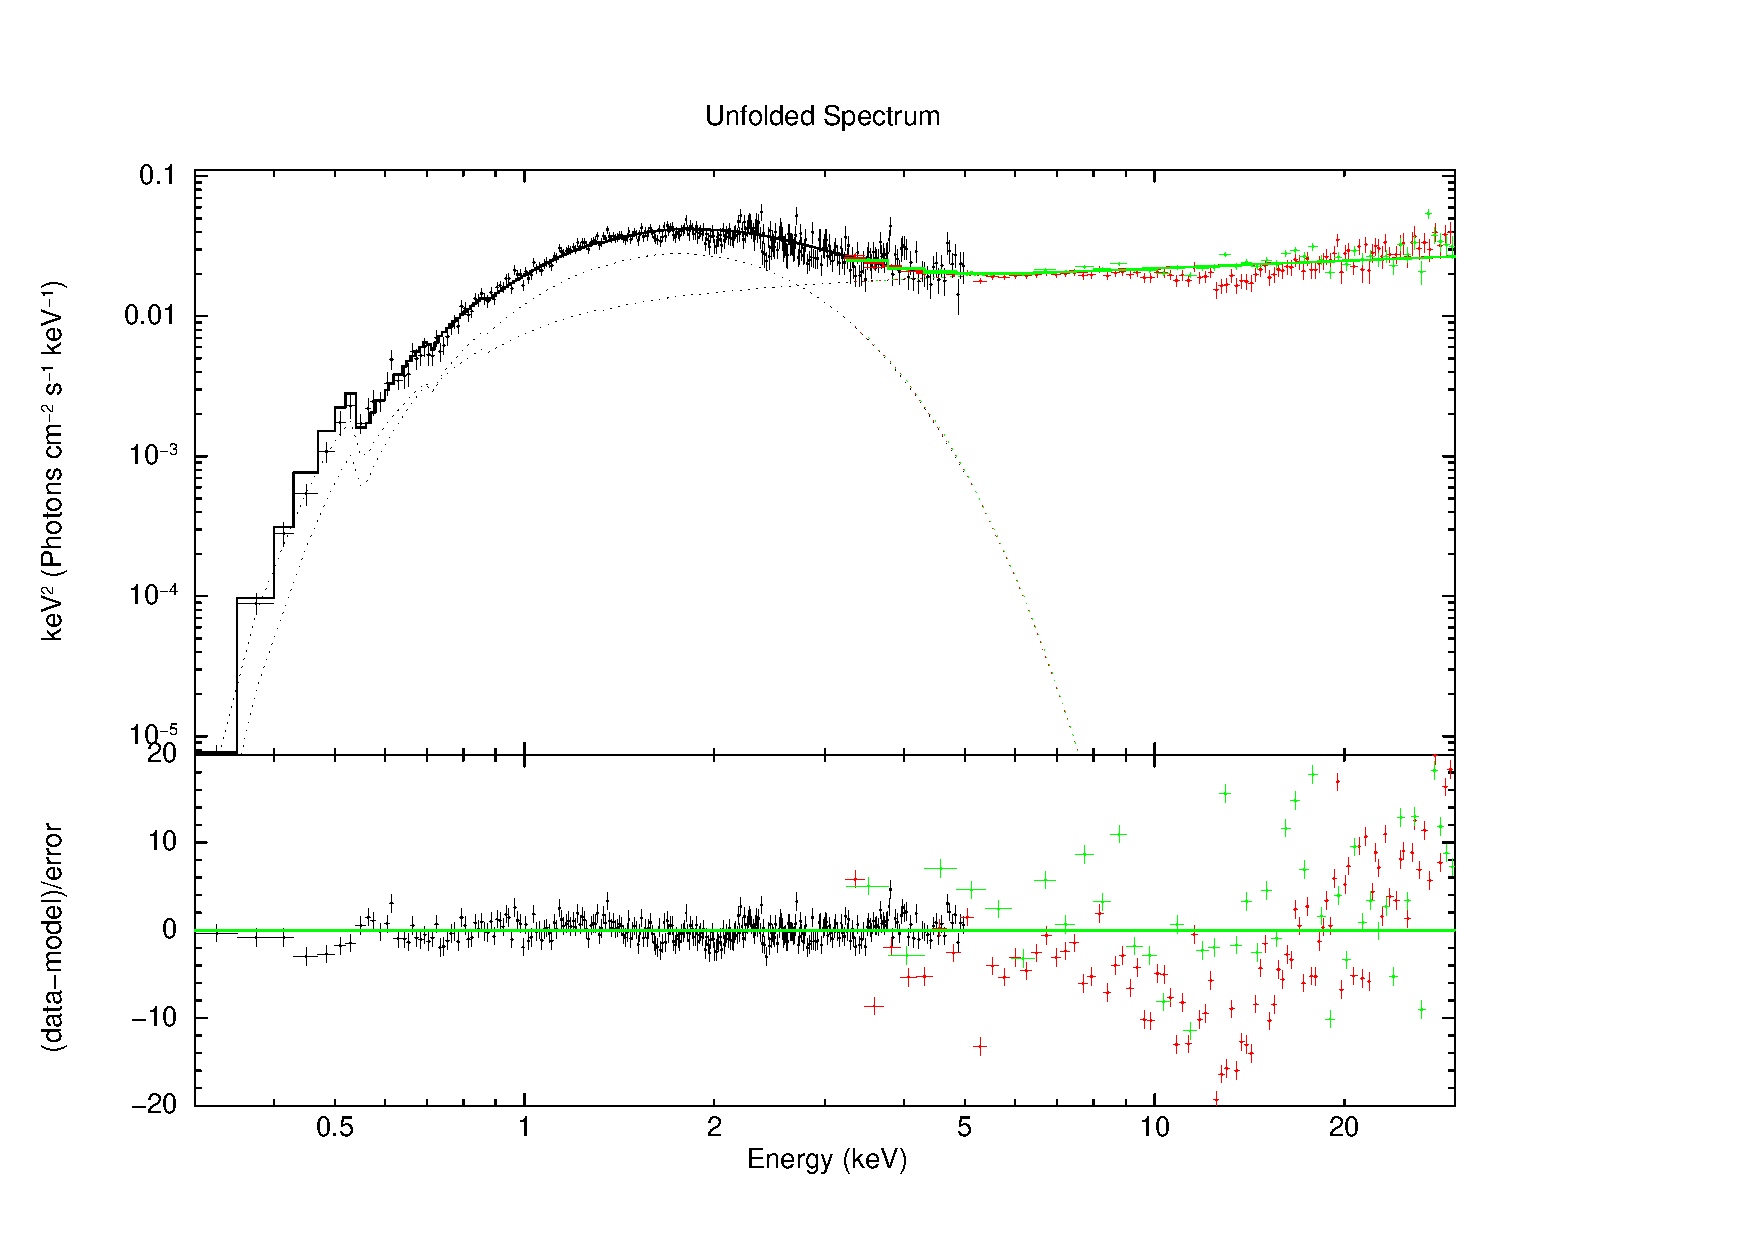
\includegraphics[width=0.8\linewidth, height=8cm]{tbabs_bbody_pow_SXT_laxpc1-2.pdf}
\caption{LAXPC2 + LAXPC1 + SXT combined Spectrum}
\label{LAXPC1+2+SXT combined spec}
\end{center}
\end{figure}
\paragraph{}
Another minor detail to note would be that time bin chosen for the data is of no concern in this case since the time element is lost when one tries to plot the energy spectrum of the data. 
\paragraph{}
Now, one might notice that the spectrum has several dotted lines as well. These are the model contributions to the data. This particular plot was made using four models with various parameters. The same one mentioned above. However, once you plot these in the /xw plotting window, you might not see the model contribution pop right up. for that you would have to use the command:
\begin{center}
\textbf{XSPEC$>$ pl eeufspec del}
\end{center}
\paragraph{}
After that and a few model parameter alterations (so that the models fit to the data in the best possible manner) we arrive at the final result. 
\paragraph{}
Now, do note that what statistics you use for the data analysis is crucial for the results to be reliable. If the data is poissonian, one cannot use $\chi^2$ statistics to fit the model. The same applies to the background. Hence usign correct statistic model is required, refer \cite{redchisquared}.








\newpage
\chapter{Background Physics}
\paragraph{}
Now that we have discussed the data processing techniques, let us first brush up on a few important concepts regarding the background physics one might need in order to understand the data received, and make sense of the numbers.
\section{Stars and their life cycles}
\paragraph{}
The story of a remnant body starts from the death of a star. This is when the nuclear fusion in the core of the star is not able to balance the immense gravitational attraction of the mass that makes it up. Hence it collapses under its own weight, much like an implosion. Let us discuss these things one step at a time. 
\subsection{What happens to the stellar core on collapse}
\paragraph{}
Let us try and understand this step by step. 
\paragraph{}
A star forms when there is enough gas, cold enough (~$10$ to $20$ $K$) to condense to such an extent that, after a certain period of darkness caused due to their temperature and low optical depth for visible light (however we do see emissions in the IR spectrum e.g. Bernard $68$ since the optical depth is wavelength dependent) and their density, and a tinge of push from any strong enough neighboring event (could be anything from supernovae explosion to fluctuations i.e. Jean's instability in the massive gas cloud etc. or, the galactic density wave interacting with a cloud), could trigger further collapse, but not nuclear burning, in this stage the star is a proto star, i.e. a dense gas cloud that is well on its way to become a star, but doesn't have nuclear fusion happening at its core. However, as more matter is pulled in and the core keeps getting hotter and hotter, eventually triggering nuclear fusion at its core. Hence, at this stage the star enters the main sequence. 
\paragraph{}
\begin{wrapfigure}{r}{0.5\textwidth}
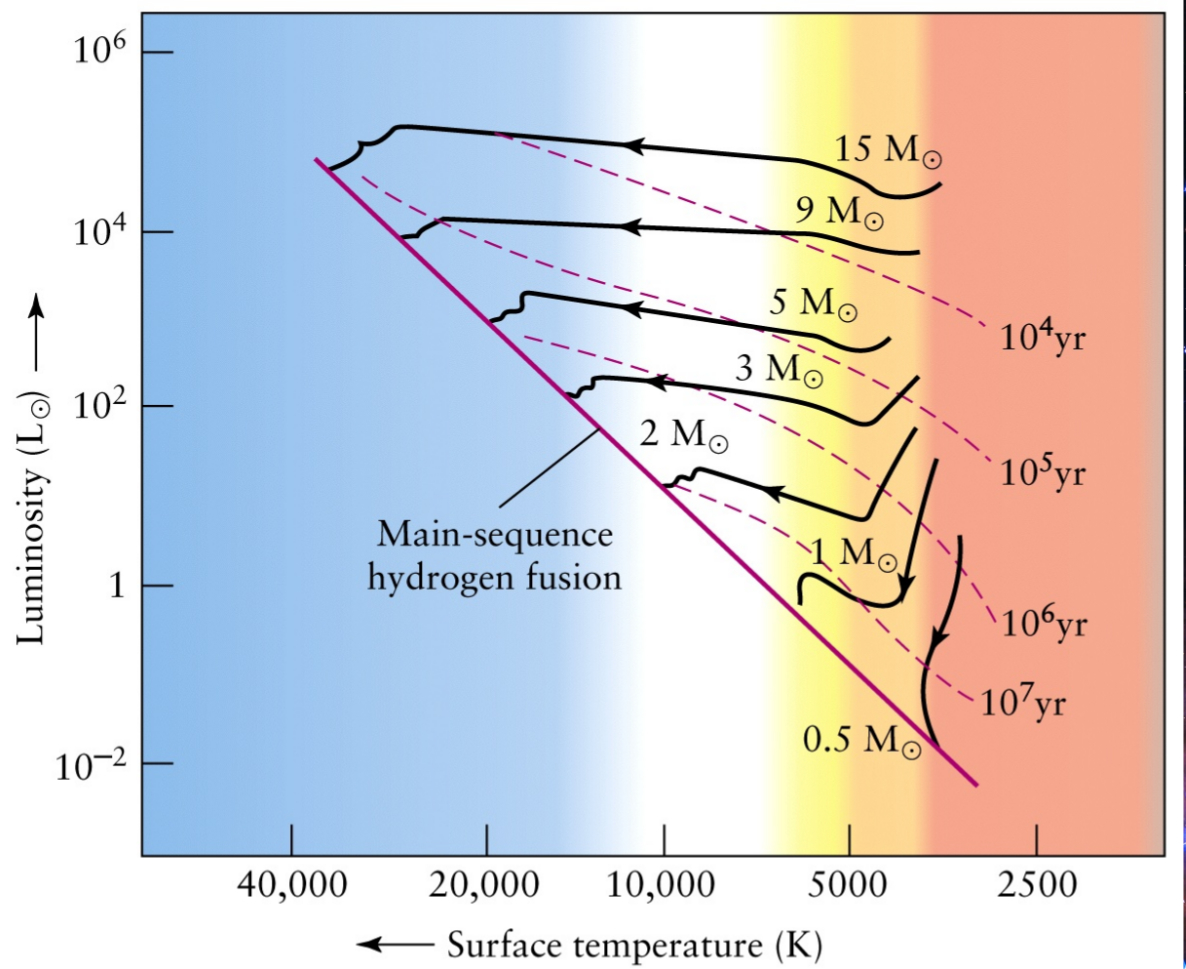
\includegraphics[width=1.0\linewidth, height=5cm]{HR_Diagram.jpg}
\caption{Star's transition from proto to Main sequence (Hayashi and Henney track)}
\label{Hayashi and henney track}
\end{wrapfigure} 
Now, depending on how much mass the proto star had when it was forming, it steps into the main sequence stage at different times (the less massive star enters the main sequence later than the high mass star since the "big one" starts burning hydrogen earlier attributed to the higher density at it's core), depending on several conditions such as the mass of the collapsing gas cloud, e.t.c. This also decides where in the main sequence the star will end up when it enters, the massive ones ending up at the upper end and the less massive ones in the lower end of the HR diagram. Note that in order for the hydrogen burning to start, the molecules would have to cross the coulomb potential barrier. However, given the temperatures at the stellar cores which are of the order of $\approx$ $10^8$ K, we could rarely expect that to happen, however, the only other mechanism that could cause fusion at such energies would be Quantum Tunneling (George Gamow, $1928$). Upon doing some Q value calculations, we can see that the maximum energy release is by hydrogen burning and it decreases all the way to iron, after which it goes to negative (i.e. in order to fuse nuclei heavier than Iron one would have a net loss in energy, in other words, one would lose energy implying no outward force to maintain a spherical shape).
\paragraph{}
\begin{wrapfigure}{r}{0.5\textwidth}
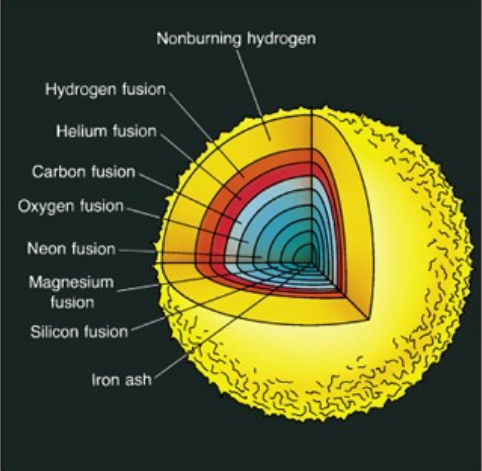
\includegraphics[width=1.0\linewidth, height=7cm]{star_shell.jpg}
\caption{Shell structure of high mass stars}
\label{Star_shell}
\end{wrapfigure}
Since the the amount of light fuel is limited within the star, (H and He are the "light" fuel, and in astronomy terms, anything heavier is termed as a metal, so oxygen is a metal, and the abundance of such elements would increase the star's "metallicity"), the product that forms when a star dies varies with what was the last thing that was burnt in it's core, which essentially dictates the consecutive outer shell composition of the star, which in turn decides the energies radiated when collapse occurs, which then would decide the luminosity of the (super/hyper) nova and would also decide what the core would end up as. Now, given the nuclear reaction chains, when hydrogen burns in it's core the star remains in the main sequence, however, the amount of hydrogen fuel in it's core is limited and hence once it runs out, the star starts to burn heavier elements, the next element being helium. Once it starts burning helium at its core, the region around the core (spherical shells called cells) gets hot enough to burn hydrogen, and hence the core now ends up burning helium and the first shell around the core starts burning hydrogen. This is when the star grows in size since now both hydrogen and helium burning increases the radiative pressure and hence causing the star to bloat. A better illustration would be to look at Figure \ref{Star_shell}. Now, one more thing to note is that the diagram shows an ideal case, in reality, because of the inhomogeneities in the star, one shell of the star may burn different elements at one time depending on several factors. All the while the star burns different fuel, it grows and shrinks in size and goes back and forth form the main sequence towards the top right side of the HR diagram (the red giant phase). This is where most of the variable stars are located at (however, this uis a debatable concept and is up for discussion). However, once the star starts to form iron in it's core, that is when stuff starts going out of hand (or limb of the star), since we loose energy while fusing iron, the star would no longer be able to push the shells and maintain it's shape, and hence, the star's core would contract (the star doesn't contract as a whole, it's just the core that does), once the core collapses, the amount of photons released causes photo-disintegration of most of the iron present in the core releasing a lot of energy (of the order of $\approx 10^8$ to $10^9$ K). 
\paragraph{}
\begin{wrapfigure}{l}{0.6\textwidth}
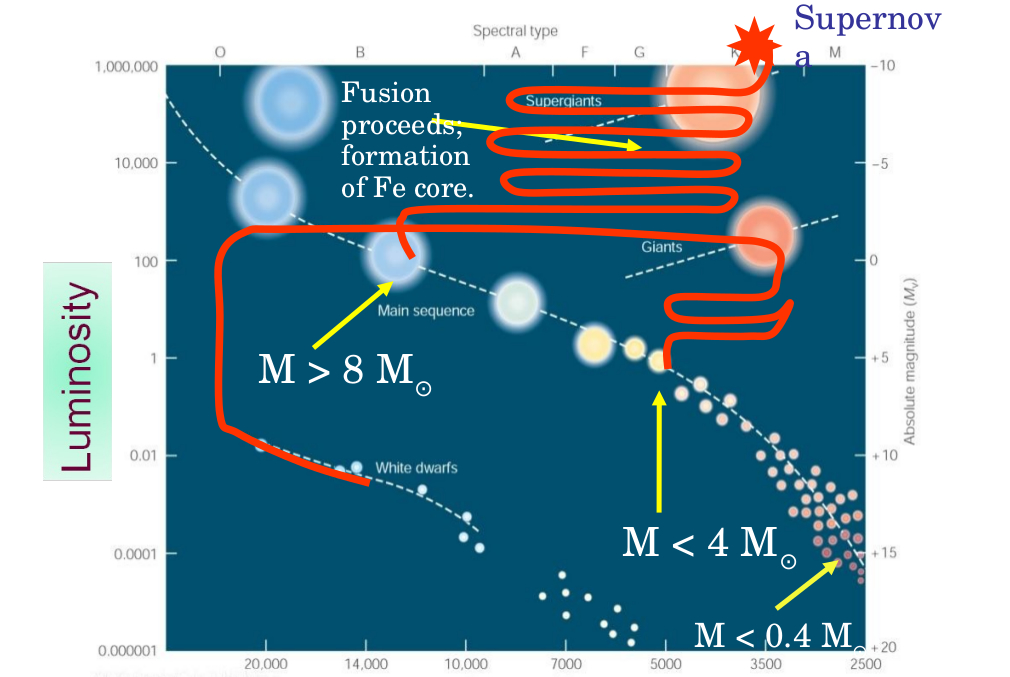
\includegraphics[width=1.0\linewidth, height=6cm]{evo_of_stars.jpg}
\caption{Story of evolution of the stars}
\label{NS_Diagram}
\end{wrapfigure}
The pressure during these times is so high that the electron degeneracy pressure can't stop it (if it is enough to halt the collapse, the remaining core forms a dwarf star), nor can the atomic structure can stop it, at this stage the electrons and protons are crushed together to produce neutrons, with a heck load of gamma radiation and neutrinos. This is when the in-falling lighter material gets ejected out (as a rebound to the in-falling heavier element that crashes into the core). This, added to the huge amounts of photons that are released during the photo-dissociation of elements in the core, causes the outer shells of the super giant to expand exponentially. This expansion causes the optical depth of the material to decrease letting the huge quantities of photons, that would otherwise be scattered and absorbed by the inner layers of the star, to be sent out into space, leading to huge flux of photons radiated at all directions. This would explain the huge EM flux radiated from the core during this process, leading to supernovae being few of the brightest events to occur in a galaxy (or maybe even the universe). This is the time when most of the heavy elements (heavier than iron and a few that are lighter) form in the universe and are scattered throughout the galaxy. 
\\
\begin{wrapfigure}{r}{0.5\textwidth}
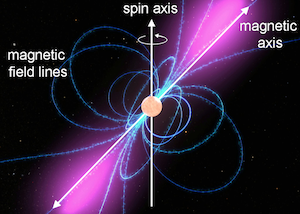
\includegraphics[width=1.0\linewidth, height=5cm]{ns_pulsar_diagram.png}
\caption{Neutron Star diagram (ref. Hayashi-Henny Track)}
\label{Star Evolution Diagram}
\end{wrapfigure}
\paragraph{}
Out of this craziness, there are several things that are born, i.e. there are several different phases of the core that is left behind. All these depend primarily on the mass of the star's core during the collapse. The fate that we are interested in is the remnant left behind after the core shrinks (because no fusion = no outward force = gravity rulez!! = shrinks the core), and not just any remnant, but a neutron star. Now, these cores, are primarily made up of neutrons, (*mention NS formation ref.*), however, the outer layers could be made up of iron left over from the core of the star. Because of this core collapse, and because the the star being an isolated body needs to conserve angular momentum, the remnant core spins up to conserve AM(*NS star spin reference enter here*). Now, one thing to note would be that neutron stars are not entirely made up of neutrons, and because of the end stages of the stellar core ending in iron, the neutron star has a thin crust of iron, this and a few other charged particles could be the reason for the magnetic field of the neutron star (*NS B field reference here*). 
\paragraph{}
\begin{wrapfigure}{l}{0.5\textwidth}
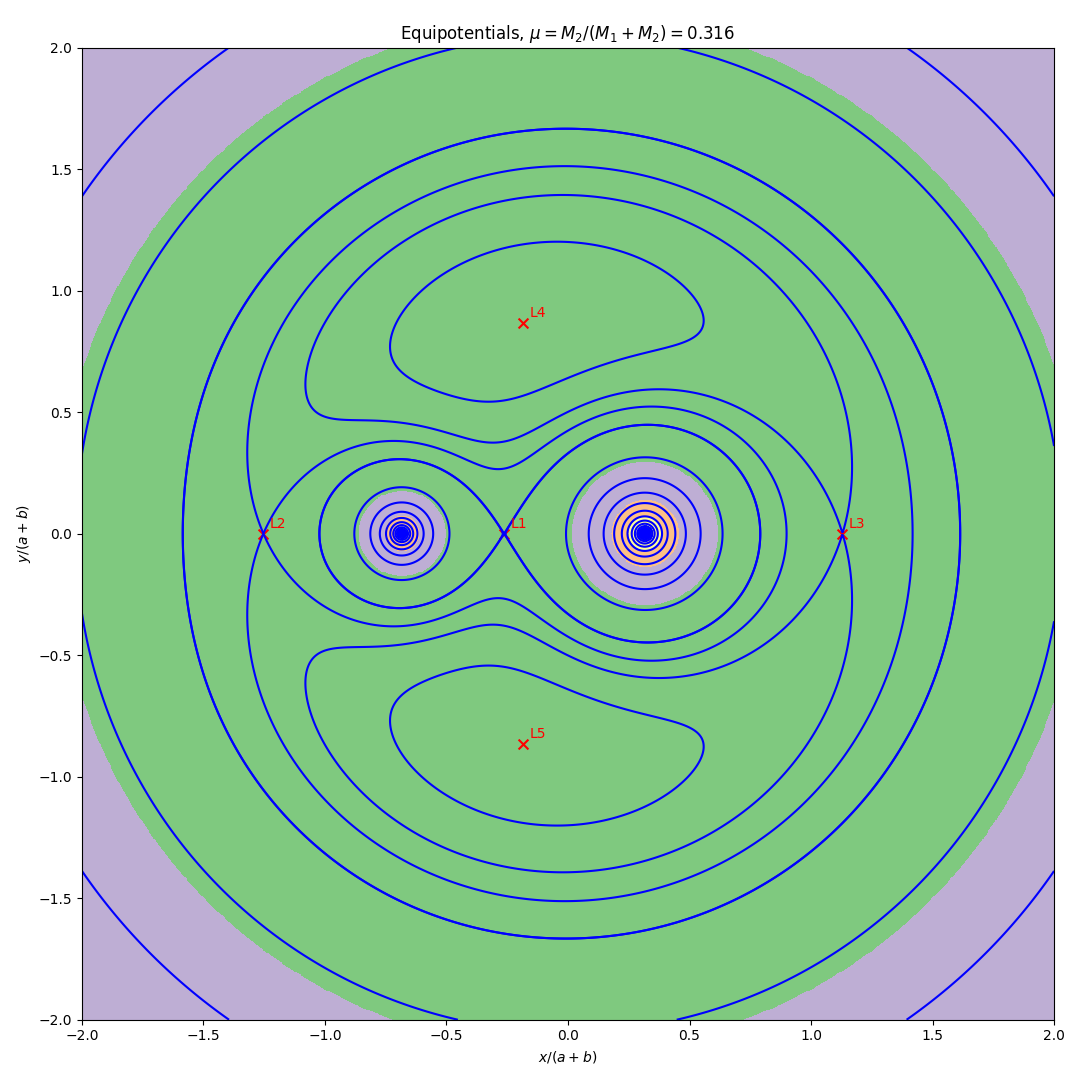
\includegraphics[width=1.0\linewidth, height=8.1cm]{equipotentials_mu_0316.png}
\caption{Equi-potential surfaces with $\mu$ = 0.316}
\label{Star Evolution Diagram}
\end{wrapfigure}
Now when the matter falls into the star, i.e. if there is any star nearby that has a size larger than it's Roche limit, (ref. two body interaction figure \ref{Star Evolution Diagram}) the extra mass (outside the lobe) spirals into the neutron star. Now, while on it's way towards the star, due to the extreme conditions (velocities, friction, etc.) while the matter falls into the neutron star, it leads to the ionization and hence emission of radiation from the neutron star and the inner regions of the accretion disk, (*Insert accretion disk reference and optical depth reference*), some of this matter that makes it to the surface leads to impart some of it's momentum to the NS causing it to spin up. There are many other things such as nuclear fusion e.t.c. that happen at the surface leading to high energy emissions such as x and gamma rays (*insert NS reference here*), and some of the charged matter that gets influenced by the magnetic fields of the star gets funneled out of the star (in the process, carrying some of the star's angular momentum away *insert NS slowing ref. here*). This funneled matter is what is detected by the radio telescopes and X ray telescopes as pulses (*insert Pulsar astronomy book ref here*), much like a light house. 
\paragraph{}
These are just some of the activities that go on within the neutron star, and the best thing is, there are several activities that I do not yet know about, hence in this project we tried to look at the photon flux and their energies to try and piece together some of the properties of the Neutron star binary. 
\subsection{Neutron star binaries}
\paragraph{}
As mentioned in the above section, we would be studying neutron star binaries. Now it is a well known fact given the abundance of stars in the galaxy, and their formation patterns, most of the stellar systems are either binaries or have more than two stars orbiting each other. Our sun being the oddity. 
\paragraph{}
Now, a neutron star binary is a system where one or more members of the system is a neutron star. These could be any number of combinations, and each of those combinations having their own formation history. Hence it would be good for now if we keep that subject aside just to keep this report short. 
\paragraph{}
However, coming back to the neutron star binaries, and the system of my work, Ultra Compact X-ray Binaries (UCXB). Now, from the huge number of neutron star binaries, there are some systems where the companion star is a star with mass $<1$ \(M_\odot\), i.e. $1$ solar mass (\(M_\odot\)). These systems could have anywhere from white dwarfs and sun like stars as companions. These kind of systems are called Low Mass Xray Binaries. X-ray since when they funnel matter into them they emit mostly in X-rays, which as mentioned above could come from neutron star surface or the inner regions of the accretion disk. Now, one might rightly argue that one can have a similar system with a black hole instead of a neutron star. However such a system would have a vastly different X-ray signature from, say the neutron star, and hence would need a separate discussion on their own, and since the object that we are concerned with in this report is a neutron star system, we would leave out the black hole alternatives to LMXBs and UCXBs. 
\paragraph{}
Now, coming back to the topic. we now know/have a brief idea about what a LMXB system is. Now, as mentioned earlier, these kinds of objects are further divided into different categories, out of those an UCXB is a system where the orbital period of the companion is so less that it completes one orbit around the neutron star in less than an hour. These kind of orbits are such that the companion star, in order to maintain the laws of relativity, would have to be extremely close to the neutron star, and hence, in most cases, the star would have matter outside it's Roche limit, and hence we would definitely see some kind of high energy emission, based again on the system. 
\section{1A 1246-588}
\subsection{What we know}
\paragraph{}
As mentioned above, $1$A $1246$-$588$ falls under the UCXB category. Now, one might ask how. Now because of the Roche lobe overflow, the mass of the companion star is low, and hence the companion star is faint in optical, however, because this matter is funneled into the neutron star, these systems glow very brightly in X rays, which is correlated to the size of Roche lobe (since the X ray flux would be a function of how much matter is falling into the NS, and hence would be related to the mass of the companion star and it's luminosity, and to a certain degree its composition). Hence by observing the structure of the spectrum and the x ray timing analysis of the source and the color-color diagram (CCD), one can see that $1$A $1246$-$588$ is a LMXB. For further proof refer t'Zand et.al.\cite{t'Zand}.
\paragraph{}
Now, there are two kinds of Neutron Star LMXB sources, i.e. the Z and the Atoll sources (Hasinger \& van der Klis $1989$). These sources have a characteristic color diagram (CCD) and hence by comparing the hard (high energy $>$ $10$ $keV$) and the soft (low energy $<$ $10$ $keV$) luminosities, one can classify between them. Now, using the CCD, it was observed that $1$A $1246$-$588$ falls under the category of an atoll source (supported by the narrative of atoll sources that they have low luminosity, and that their phase doesn't change as often as other sources).
\paragraph{}
Now, apart from the fact that it is a candidate UCXB, we also know that this is one of the faintest UCXBs, with an absolute magnitude of M$_V$=$3.4$ -- $4.0$ (Jonker et.al. 2006), i.e. absolute magnitude of the optical counterpart of 1A 1246-588. This also suggests (van Paradijs \& McClintock 1994) that these systems are UCXBs, since here the faintness of the counterpart is due to the re-possession of the X-rays in a physically small accretion disk. 
\paragraph{}
This is further supported by the fact that optical spectroscopic data does not show hydrogen features (Zand et al. 2008) which is in support of it being an UCXB (by Bassa et al. 2006). The same paper (Zand et al. 2008) also notes that since there are no persistent dips (eclipses) in the X-ray flux implying that the inclination angle is at most 70$^o$ (Horne 1985). The correlation factor which is used to derive the accretion flux (as mentioned, periodic dips in the X ray luminosity due to eclipsing caused by the companion star), from the observed flux, is at most 3 (=1/cos70$^o$). Combining both uncertainties, the ratio between the persistent flux and the Eddington limit is accurate to within a factor of 4. This being a constrained measurement since it is significantly below the 2\% mark, a regime in which a source is said to be UCXB, further confirming that 1A 1246-588 is an UCXB (t'Zant et al. 2007). 
\paragraph{}
This is qualitatively explained by the smaller accretion disks in UCXB needing a smaller irradiation flux to remain in a hot high viscosity state, that sustains accretion into compact object (van Paradijs 1996). For a much more detailed reference, refer the paper by 't Zand et al. 2008 \cite{t'Zand}.
\paragraph{}
Now, we also know that this object has a Kilohertz QPO at 1258 KhZ, with a single trial significance of more than 7 $\sigma$(Jonker et al. 2007) in the soft high flux state. However this was not observed in our data, more on that later. The same paper also confirmed, using spectral properties that the object is an atoll source. This paper also reports the mass limits of the neutron star to be at M$_{NS} < 1.75 M_{sol}$ and R $<$ 15.5 kilometers. The same paper also reported that during the low-flux stage, it's spectrum resembles that of the crab.
\paragraph{}
These along with several other points were to be, first, verified and then built upon.
\subsection{My work on $1$A $1246$-$588$}
\paragraph{}
Predominantly when one receives data, there are two things to be done, with it, namely spectral analysis, where one looks at the energy spectrum of the source, and the temporal analysis (also known as the timing analysis) wherein we look a the change of flux throughout the duration of the observation. These two analysis are completely different since we cannot perform energy spectral analysis using timing data, and similarly we cannot perform timing analysis using energy spectrum. 
\paragraph{}
Now, we start with the temporal analysis, from which we can determine the classification of the source, which would then let us take the further steps. Upon first plotting the CCD, we can very clearly see that the source is an atoll source, along with being primarily in the soft state:
\begin{figure}[h]
\begin{center}
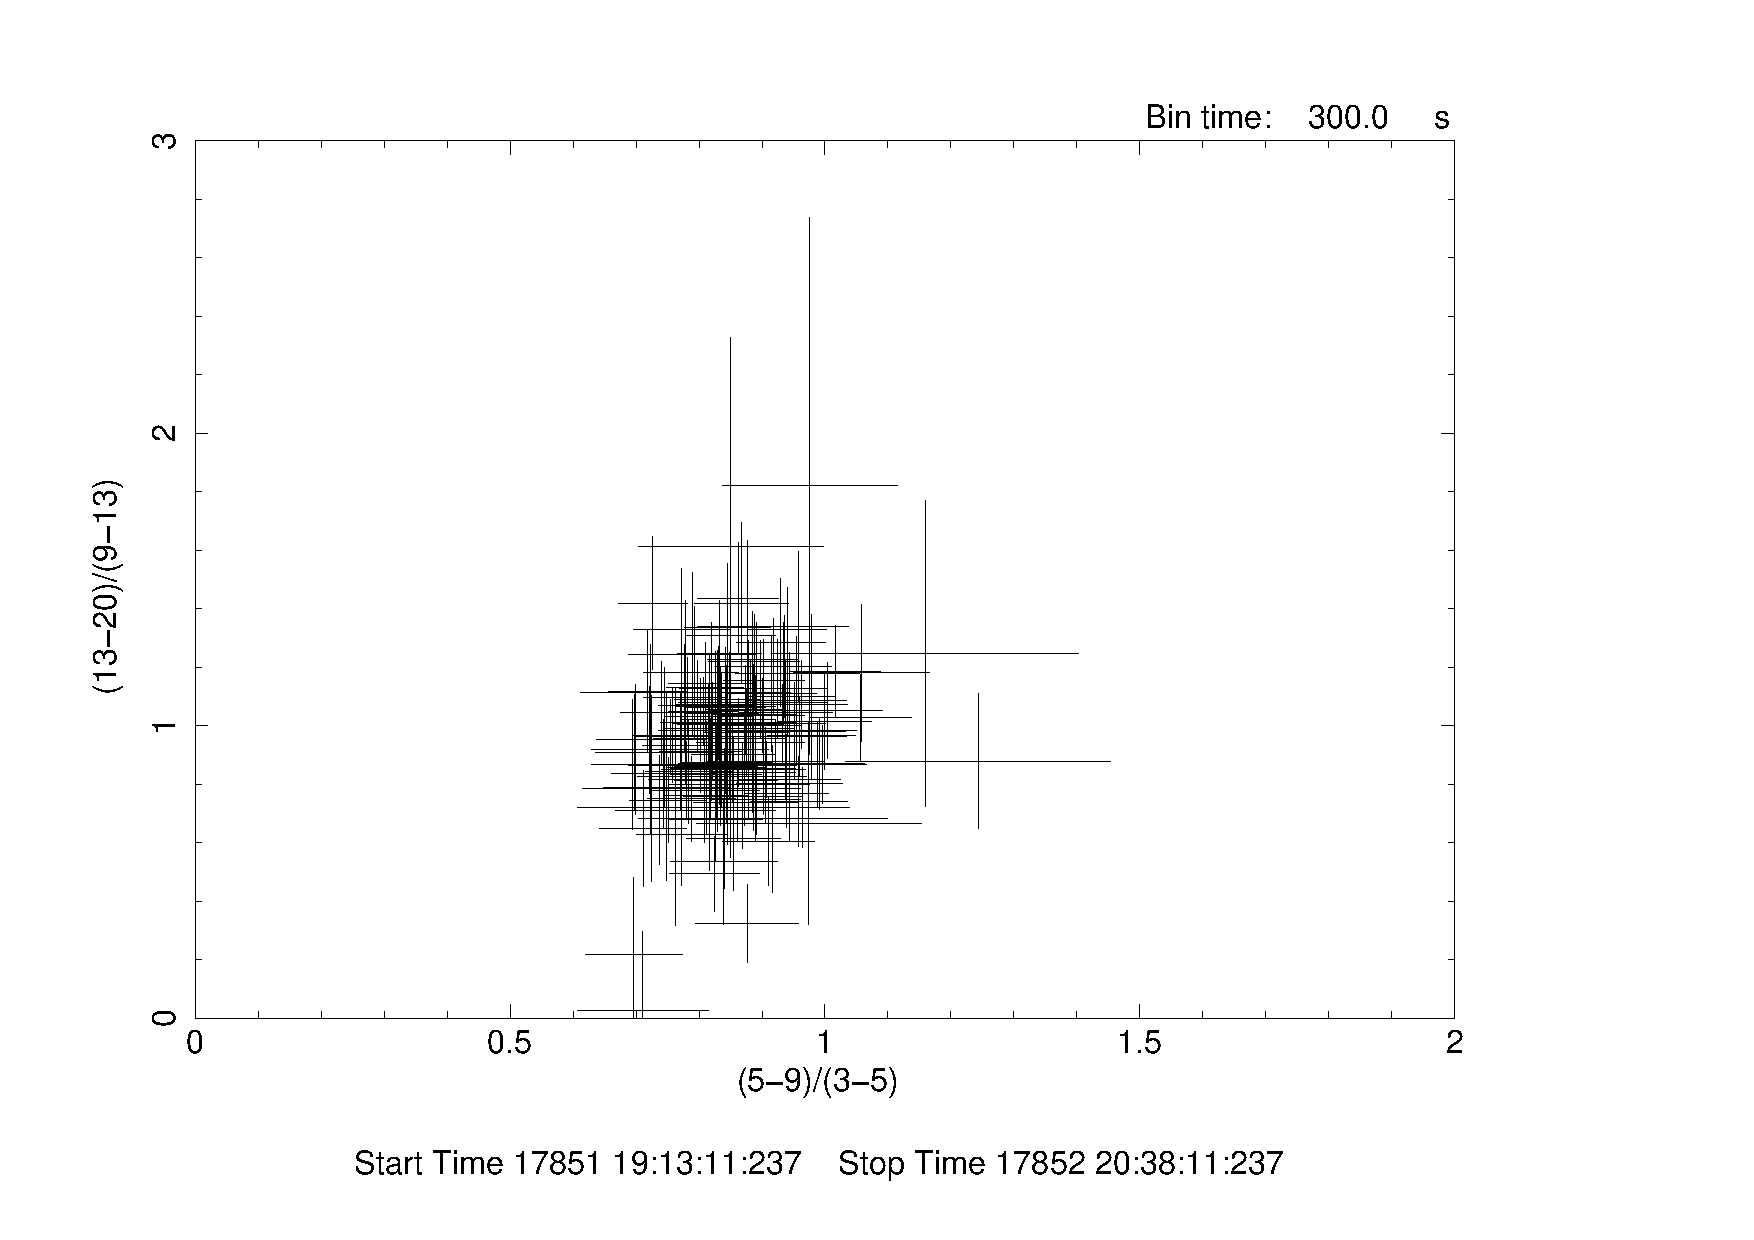
\includegraphics[width=0.8\linewidth, height=8cm]{CCD_300.pdf}
\caption{CCD with 300 second time bin. This figure clearly shows the atoll nature of the source.}
\label{CCD_300s}
\end{center}
\end{figure}
\paragraph{}
Now, the pooints with huge error bars are the outliers with huge intensity variations. Other than that, the rest is from the source. We can clearly see that most of the data points lie below 1 along the x axis, signalling towards a higher intensity in the soft x-ray band. We can also see that most of data points are around 1 in the hard energy axis, signalling that the source doesn't change much in the hard energy range. 
\paragraph{}
Given that the source doesn't change much during the observation, we do not have different phases, and hence phase resolved spectroscopy becomes pointless since all of them would yield the same results. Note that figure \ref{CCD_300s} is obtained using the lightcurves of the same instrument (LAXPC), hence no need for normalization. Also, given the above we now need to plot the power spectrum so that if there are any oscillations in the data, possibly produced because of oscillations in the data, we would be able to see them. I plot the powerspectrum using powspec as shown in \ref{Powspec_1s}.
\begin{figure}[h]
\begin{subfigure}{0.48\textwidth}
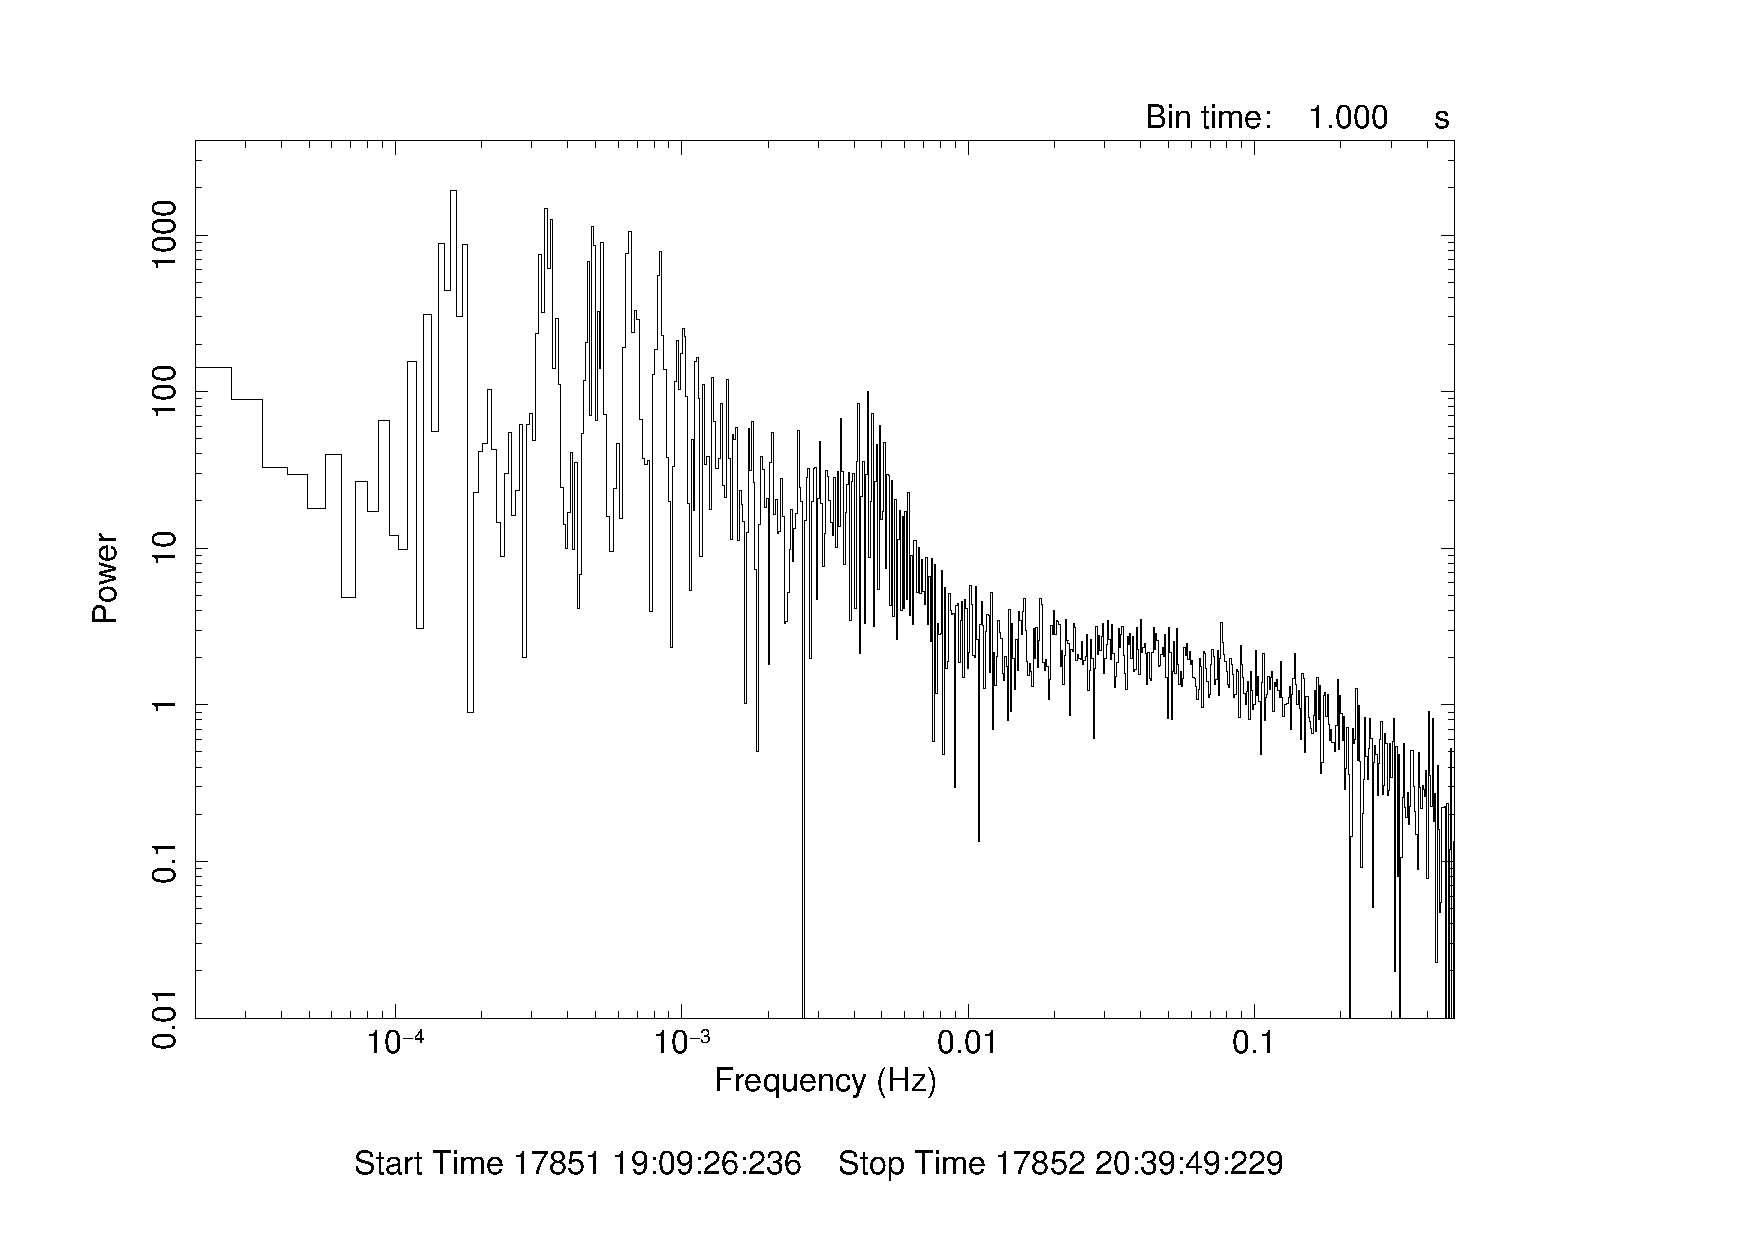
\includegraphics[width=1.0\linewidth, height=7.5cm]{powspec_1s.pdf} 
\caption{Powspec plot with Nyquist frequency 0.5 Hz}
\label{Powspec_1s}
\end{subfigure}
\begin{subfigure}{0.48\textwidth}
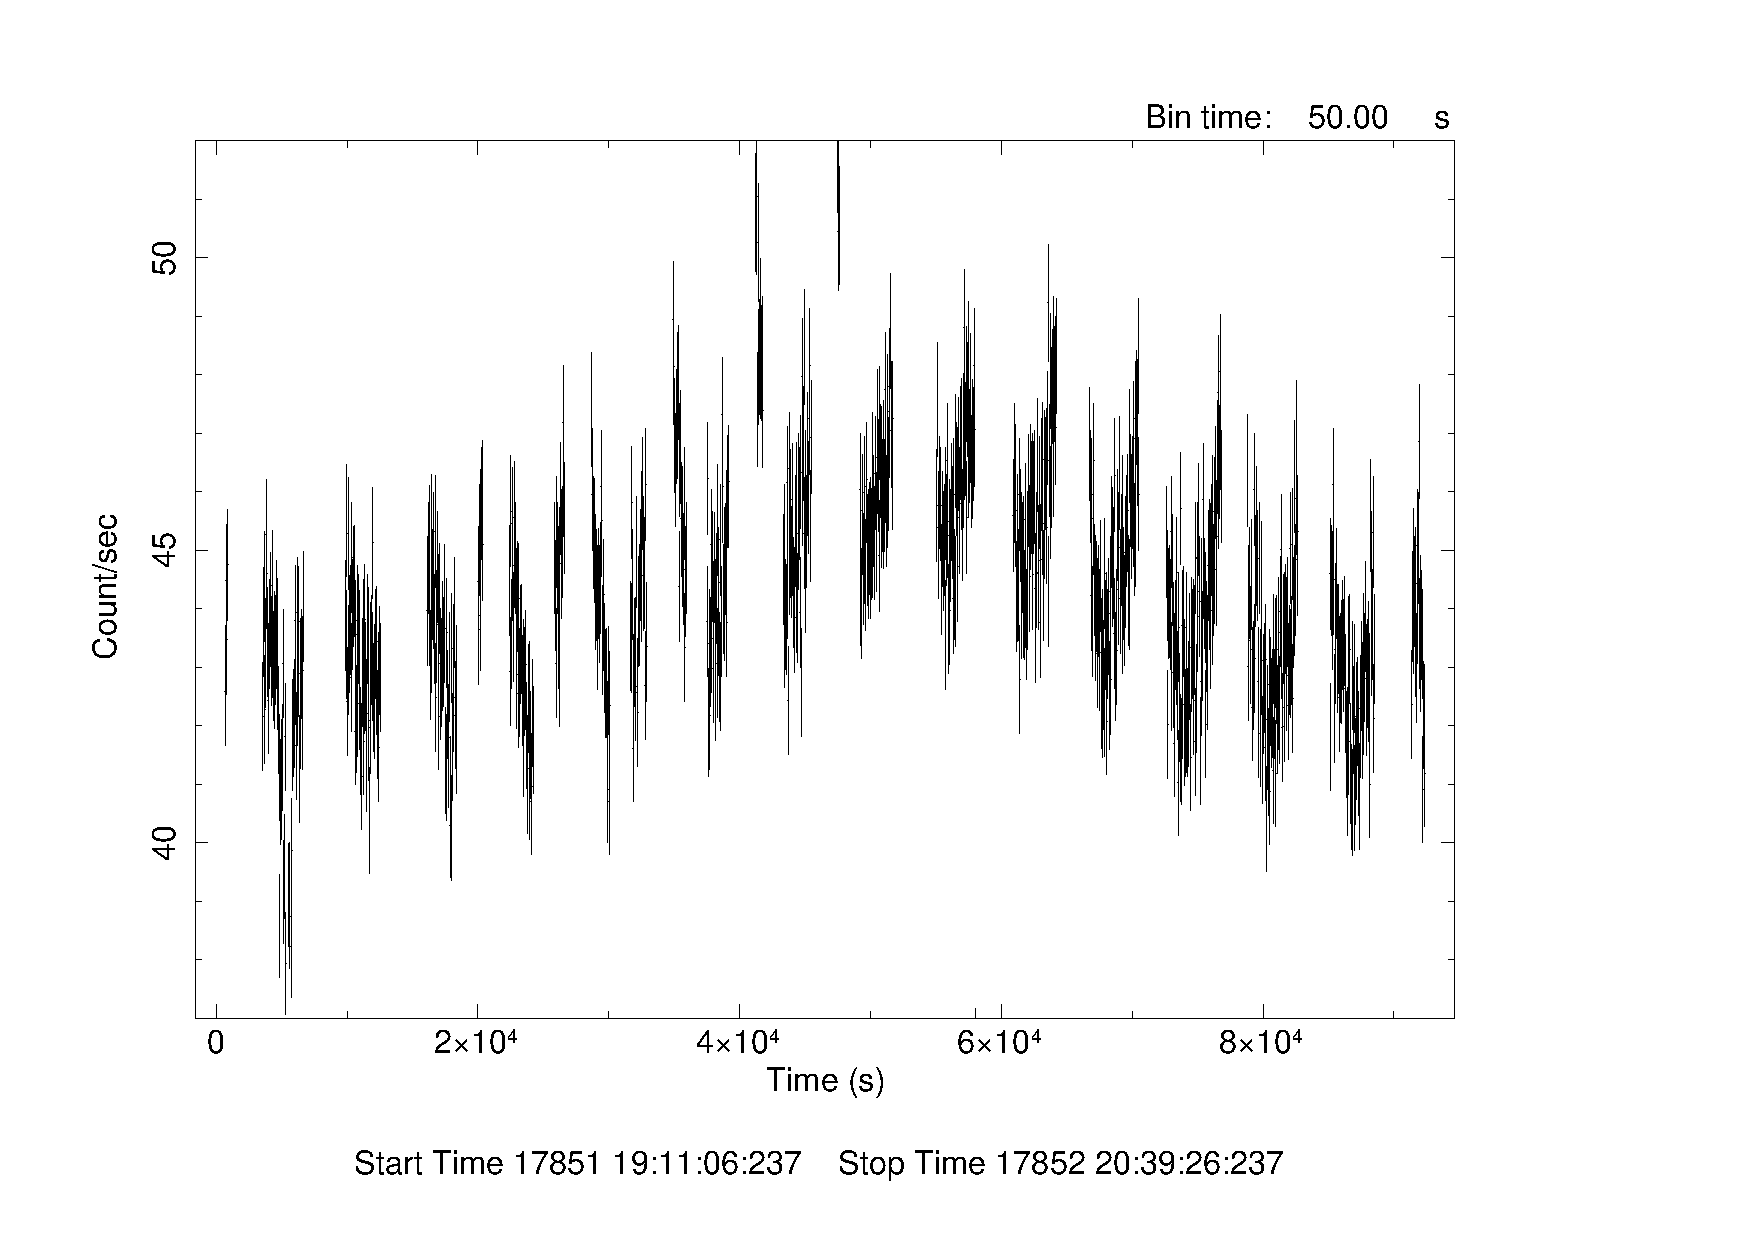
\includegraphics[width=1.0\linewidth, height=7.5cm]{LXPC2_50s.pdf}
\caption{50 second background corrected light curve using LAXPC. Here we can see the intensities rise and fall over each GTI.}
\label{LAXPC2_LC_50s}
\end{subfigure}
\caption{LAXPC Power spectrum for 1 second bin time and 50 second light curve.}
\end{figure}
\paragraph{}
The above figure is the Leahy normalized power spectrum. We see several peaks between 10$^{-4}$ and 10$^{-3}$ Hz. However, those peaks are the peaks due to the oscillations generated in the data because of the satellite passing through SAA. The flux increases each time the satellite approaches SAA and decreases when it goes away. This can be seen in figure \ref{LAXPC2_LC_50s}. 
\paragraph{}
We can also see that there seems to be a QPO like peak in the power spectrum, however, there is a strong probability that that peak is because of the gaps in light curve which can be seen in the 50s time binned version of the same. 
\paragraph{}
Apart from this, in the light curve, we also see a net rise and fall in intensity. However, turns out, this feature is present in all LAXPC data. It is prominent here since the source flux is so low that it is not discernible from the background. Apart from all these, we can also see that the light curve is mostly featureless, and so is the power spectrum. 
\paragraph{}
We also look at the hardness intensity diagrams of both the energy ratios and find a similar pattern, and it also reinforces our initial claim that the source is emitting primarily in the soft xray regime. \\
\begin{figure}[h]
\begin{subfigure}{0.48\textwidth}
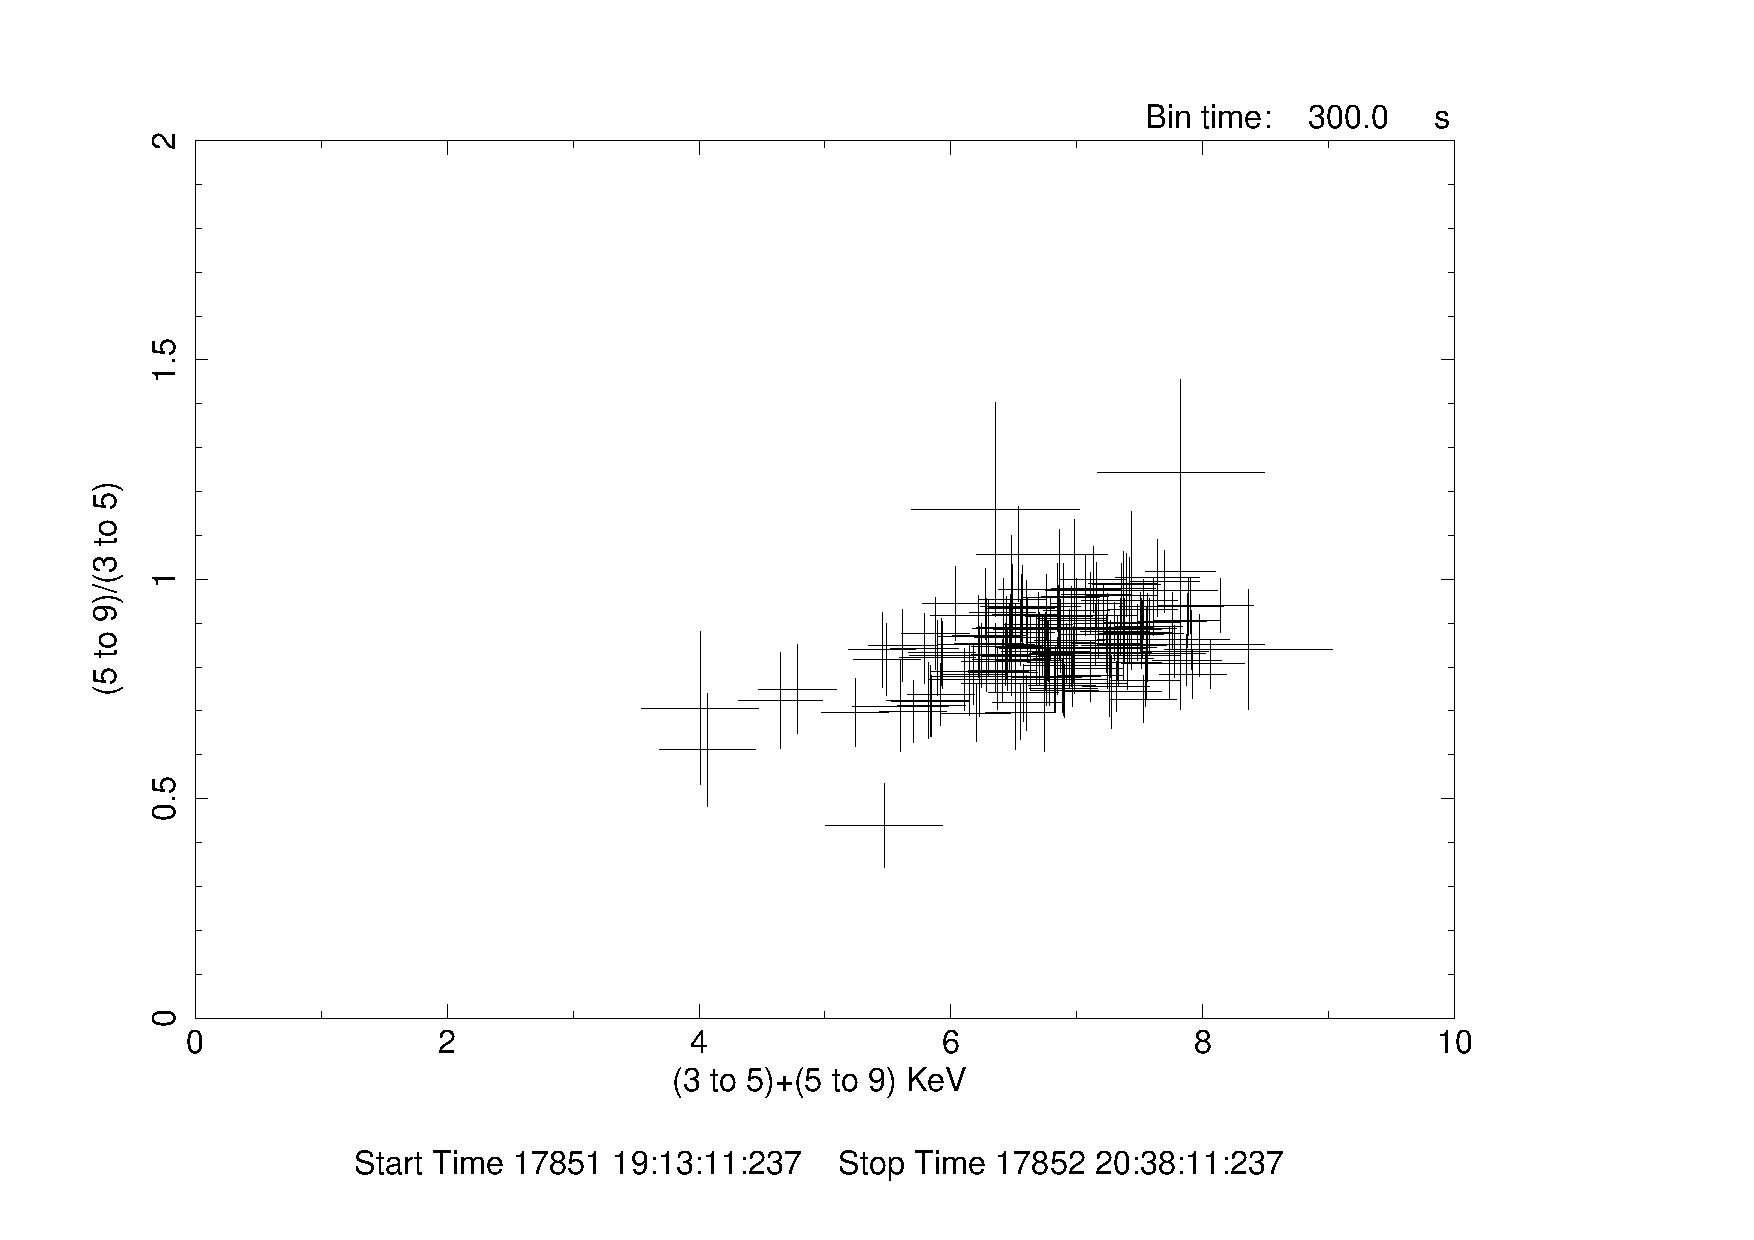
\includegraphics[width=1.0\linewidth, height=7.5cm]{3-5_5-9_HID_300s.pdf}
\caption{HID of 3-5 KeV and 5-9 KeV light curves}
\label{HID1_300s}
\end{subfigure}
\begin{subfigure}{0.48\textwidth}
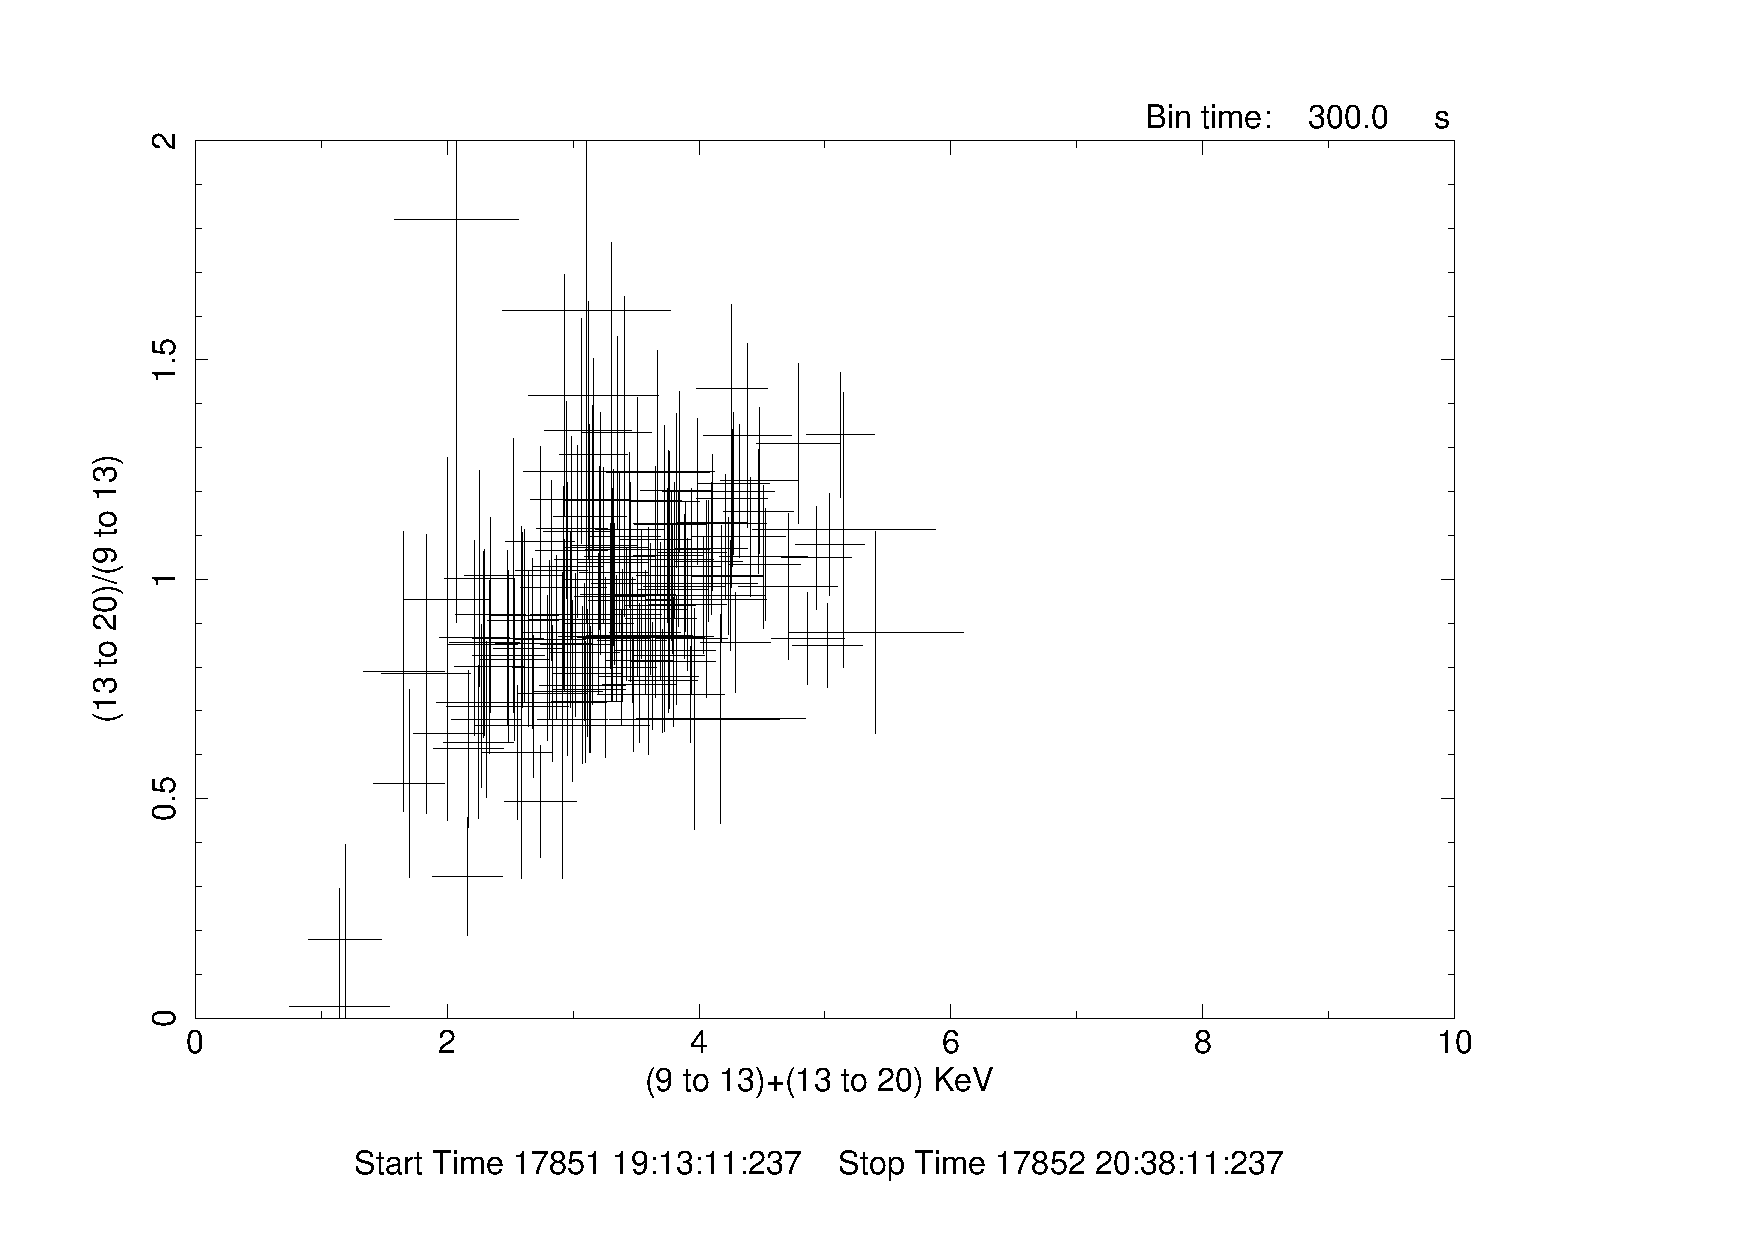
\includegraphics[width=1.0\linewidth, height=7.5cm]{9-13_13-20_HID_300s.pdf}
\caption{HID of 9-13 KeV and 13-20 KeV light curves}
\label{HID2_300s}
\end{subfigure}
\caption{HID plots of both the energies with 300 second time bins. This signals towards our earlier hypothesis that the source is emitting primarily in the soft x-ray regime}
\end{figure}
\paragraph{}
Coming to the spectral analysis. For starters, while performing the spectral analysis, I used both LAXPC 1 and 2 data for energy ranges higher than 3 KeV and, SXT data for energy ranges higher than 0.3 KeV up till 5 KeV. Since there are multiple detectors involved, we need a constant factor, hence in all the model fittings a constant factor was considered. Other than that, we used the solar abundance tables by Lodders et.al (2003). with the absorption crossection according to Balucinska-Church \& McCammon (1992). Also, since the data is mostly poissonian, we have used poissonian statistic for the spectrum and gaussian for the background. The joint SXT and LAXPC results are as follows:
\begin{table*}
\begin{small}
\caption{Summary of joint SXT and LAXPC energy spectrum without grouping}
\label{tab:spec_sxt_laxpc_3-25KeV_1}
\begin{center}
\begin{tabular}{p{3cm}cc}
\hline \hline
Fitting parameters.                             & \texttt{BBody + Powerlaw}           & \texttt{DiskBB + Powerlaw}       \\ \hline \hline
nH ($\times 10^{22}$)                           & $0.40_{-0.02}^{+0.02}$            &$0.56_{-0.02}^{+0.02}$          \\
$T_{in}, kT (KeV)$                              & $0.41_{-0.01}^{+0.01}$            &$0.53_{-0.01}^{+0.01}$         \\
$\alpha$ PhoIndex                               & $1.82_{-0.01}^{+0.01}$            &$1.79_{-0.02}^{+0.02}$         \\\hline
$norm \ Powerlaw$                                 & $1.46E-2_{-0.48E-2}^{-0.49E-2}$   &$0.0137_{-0.4E-2}^{+0.5E-2}$        \\ \hline
$norm \ Comptt/BBody$                             & $9.03E-4_{-4.90E-5}^{+5.13E-5}$   &$70.19_{-8.52}^{+9.67}$    \\ \hline
Flux($10^{-10}$ erg~cm$^{-2}$ s$^{-1}$)        & $21.79$                           &$21.77$                       \\
\hline \hline
pgstat/dof/BIC                                  &  1390/615/1428                    & 1333/615/1372               \\
\hline \hline
\end{tabular}
\end{center}
\end{small}
\end{table*}
\paragraph{}
First, as per \cite{t'Zand} The spectrum of 1A 1246-588 fit well with the comptonized model, however, what we noticed that the comptonized model did not fit well with the data. However, I tried to fit the aforementioned models \texttt{BBody+Powerlaw} and \texttt{DiskBB+Powerlaw} with the data and the fitting parameters are as shown in table \ref{tab:spec_sxt_laxpc_3-25KeV}. Note that in order to compare the fit I used Bayesian Information Criteria (BIC) \cite{BIC1} since the data that I used was poissonian in nature. 
\paragraph{}
After binning the data to make it gaussian, I performed the same analysis on the grouped data to obtain the parameters shown in table \ref{tab:spec_sxt_laxpc_3-25KeV_2}.
\begin{table*}
\begin{small}
\caption{Summary of joint SXT and LAXPC energy spectrum with grouping (Poissonian data converted to gaussian)}
\label{tab:spec_sxt_laxpc_3-25KeV_2}
\begin{center}
\begin{tabular}{p{3cm}cc}
\hline \hline
Fitting parameters.                             & \texttt{Gabs*Powerlaw + compTT}   & \texttt{Gabs*Powerlaw + DiskBB} \\ \hline \hline
nH ($\times 10^{22}$)                           & $0.43_{-0.07}^{+0.04}$            &$0.57_{-0.03}^{+0.02}$         \\
$T_{in}, kT (KeV)$                              & $38.47_{-}^{-}$                 &$0.52_{-0.03}^{+0.02}$         \\
$T_0$                                           & $0.31_{-0.02}^{+0.02}$            & ---                         \\
$\alpha$, PhoIndex                              & $1.70_{-0.06}^{+0.05}$            &$1.76_{-0.03}^{+0.03}$         \\\hline
$norm \ Powerlaw$                                 & $1.09E-2_{-1.59E-3}^{+1.57E-3}$   &$1.31E-2_{-0.86E-3}^{+1.21E-3}$\\ \hline
$norm \ Comptt/BBody$                             & $1.27E-3_{-}^{-}$               &$79.85_{-20.49}^{+23.82}$   \\ \hline
$\tau_p$                                        & $1.78E-2_{-}^{-}$               & ---   \\
\hline \hline
$\chi^2$(dof)                                   &  1.22(479)                        & 1.19(481)               \\
\hline \hline
\end{tabular}
\end{center}
\end{small}
\end{table*}
\paragraph{}
I also introduced a model to account for the slight absorption at $\approx$12 KeV (using a gaussian absorption model \texttt{Gabs}) since it looked like there was some absorption feature at that energy. After a bit of searching, that feature turned out to be an artefact due to LAXPC. The mentioned plots are as shown in figure \ref{Spec2}.
\begin{figure}[h]
\begin{subfigure}{0.48\textwidth}
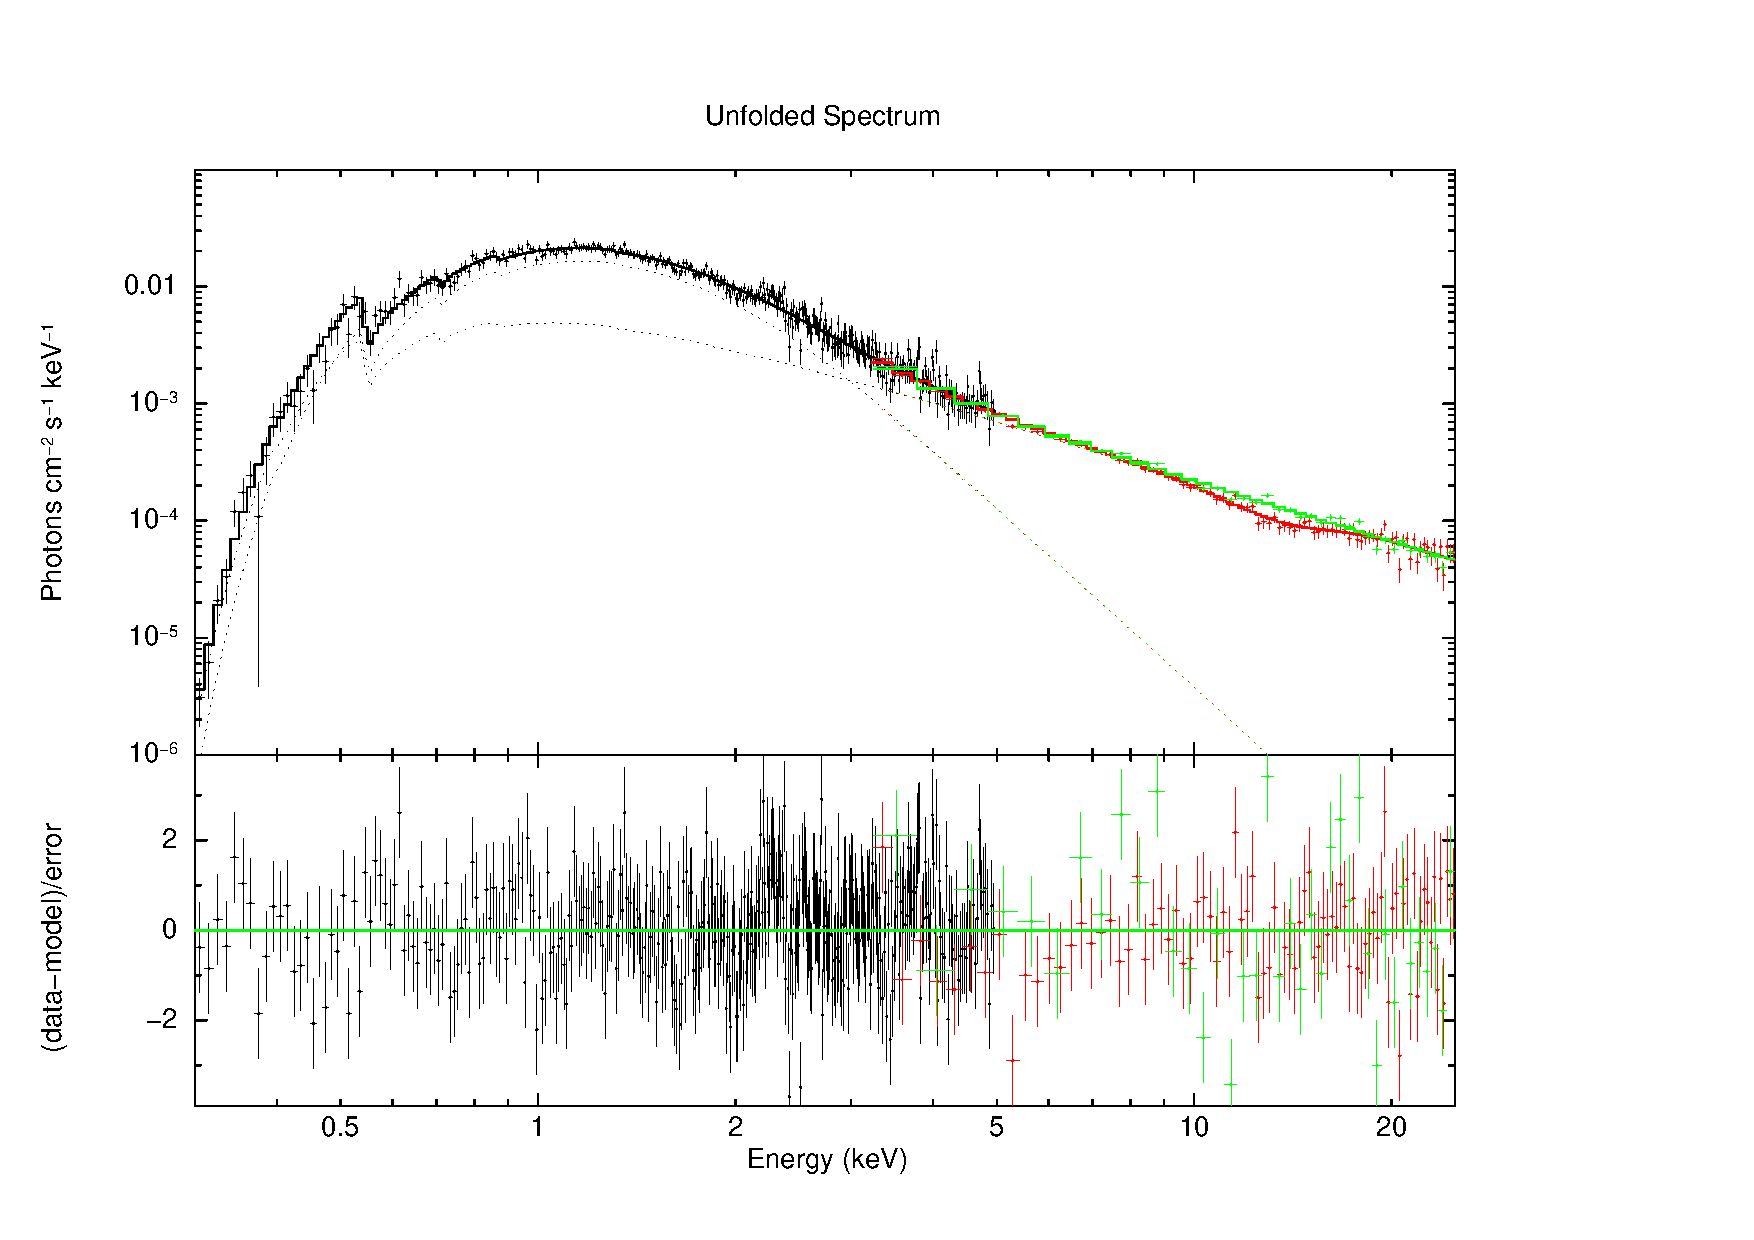
\includegraphics[width=1.0\linewidth, height=7.5cm]{tbabs_gabsPl+comptt.pdf}
\caption{\texttt{Gabs*Powerlaw + compTT} energy spectrum}
\label{Spec3}
\end{subfigure}
\begin{subfigure}{0.48\textwidth}
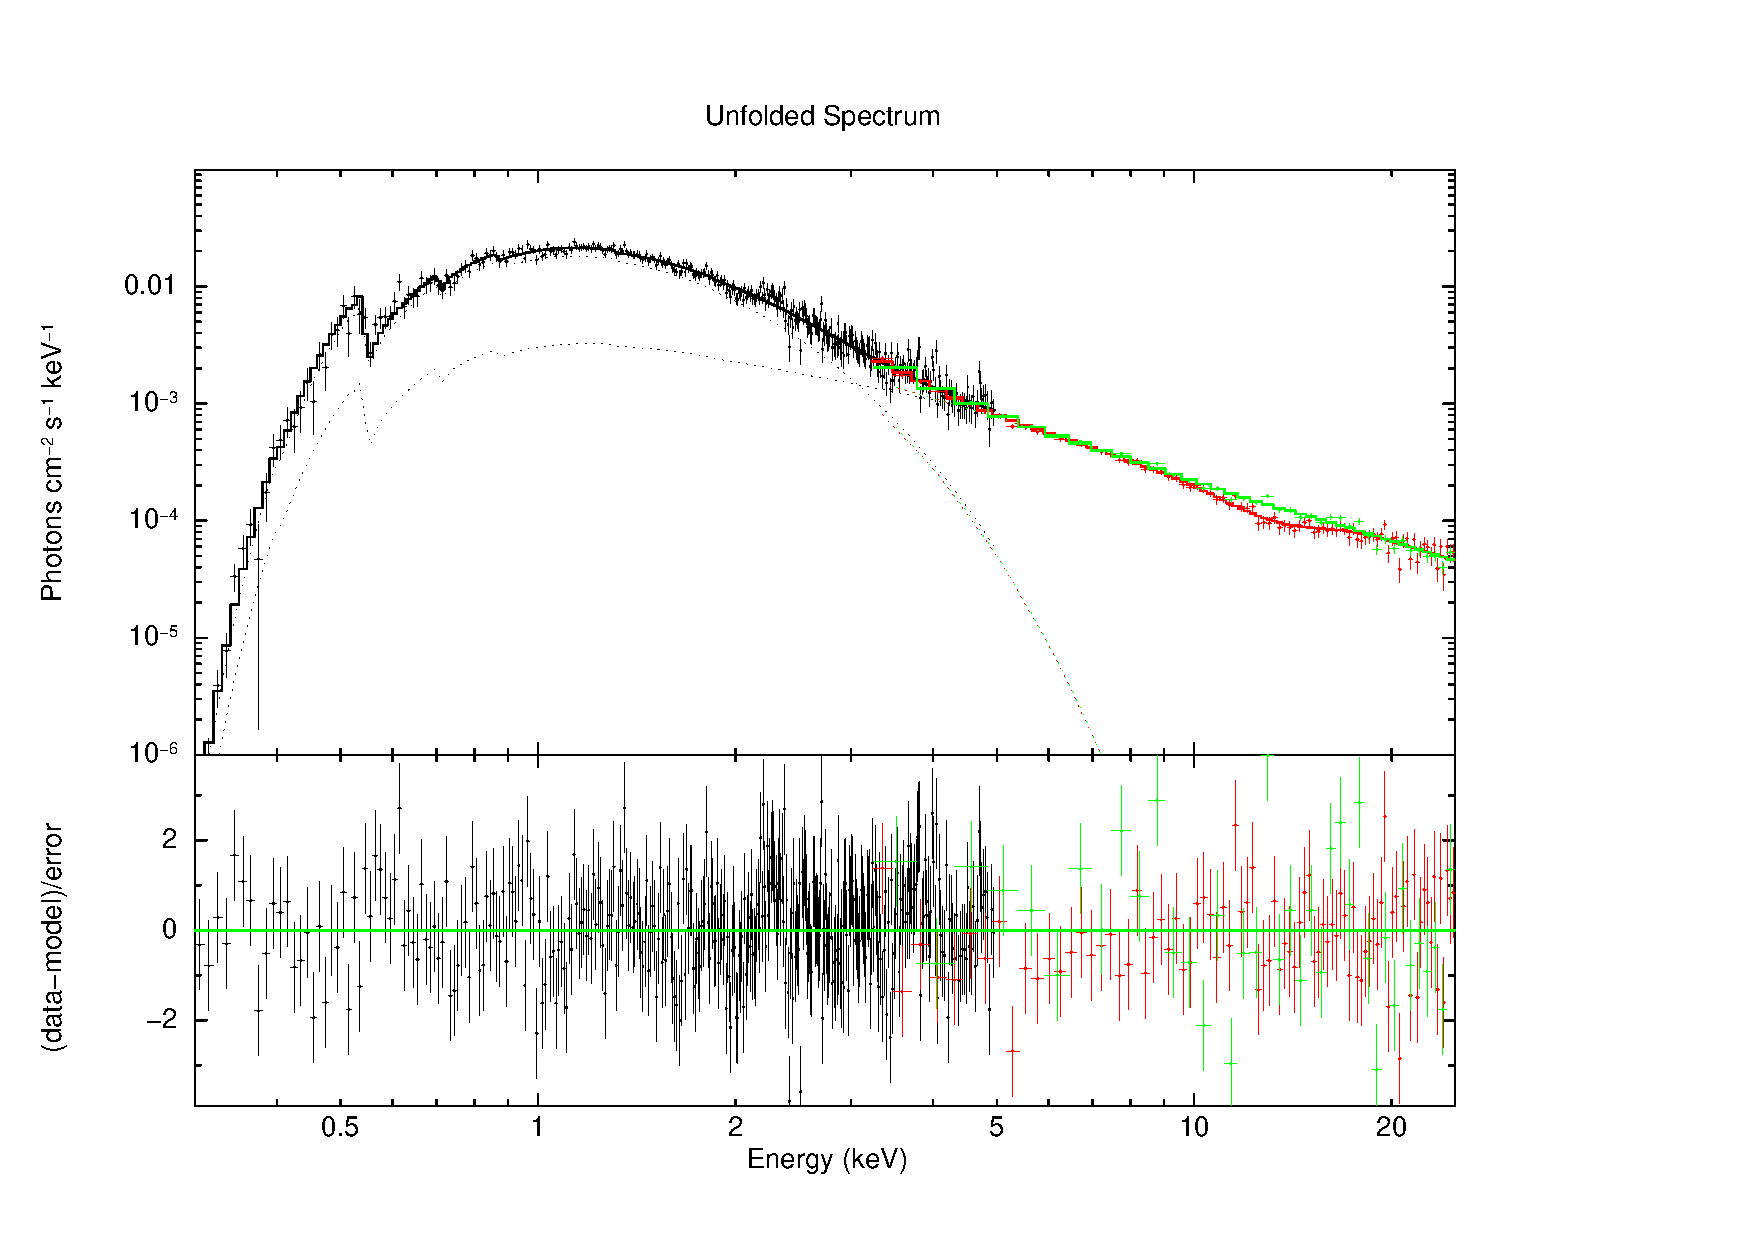
\includegraphics[width=1.0\linewidth, height=7.5cm]{tbabs_gabsPl+diskbb.pdf}
\caption{\texttt{Gabs*Powerlaw + DiskBB} energy spectrum}
\label{Spec4}
\end{subfigure}
\caption{Spectral plots for the table \ref{tab:spec_sxt_laxpc_3-25KeV_2}}
\label{Spec2}
\end{figure}
\paragraph{}
To conclude the work, the timing properties of the source remain largely inconclusive partly due to the low luminosity of the source, apart from that the spectrum of the source gives information about several parameters of the source such as the thermal temperature of the inner portion of the disk, the number of hydrogen, the seed photon temperature etc. I am still wroking on understanding the data, and what the results of the spectral analysis mean, hence this is a work in progress. 
\paragraph{}
Now, the next step of the timing analysis would be to plot the current CCD with the CCD obtained from RXTE, which is taken over an extended period of time which would give us information about what was the phase of the source during observation. This along with a strong theorotical understanding of the astrophysical phinomena would give me a deeper understanding of the source 1A 1246-588. 









\begin{thebibliography}{20}

\bibitem{KlisImp}Klis, van der. “Fourier Techniques in X-Ray Timing.” NATO Advanced Study Institutes Series. Series C, Mathematical and Physical Sciences, Anton Pannekoek Institute for Astronomy (API), 1 Jan. 1988, dare.uva.nl/search?identifier=41d71571-7c62-4ef4-871d-87cfbfec499e.
\bibitem{SB}Bhattacharyya, Sudip. “X-Ray Views of Neutron Star Low-Mass X-Ray Binaries.” [1002.4480] X-Ray Views of Neutron Star Low-Mass X-Ray Binaries, TIFR, 24 Feb. 2010, arxiv.org/abs/1002.4480.
\bibitem{Galloway}Galloway, et al. “Intermittent Dipping in a Low-Mass X-Ray Binary.” [1607.00074v1] Intermittent Dipping in a Low-Mass X-Ray Binary, Monash University, 30 June 2016, arxiv.org/abs/1607.00074v1.
\bibitem{Klis1}Klis, van der. “The Z/Atoll Classification.” SAO/NASA ADS: ADS Home Page, 1 Nov. 1989, adsabs.harvard.edu/abs/1989ESASP.296..203V.
\bibitem{Klis2}Jonker, et al. “Detection of a 1258 Hz High-Amplitude Kilohertz Quasi-Periodic Oscillation in the Ultra-Compact X-Ray Binary 1A 1246-588.” [0704.1741v1] Detection of a 1258 Hz High-Amplitude Kilohertz Quasi-Periodic Oscillation in the Ultra-Compact X-Ray Binary 1A 1246-588, 13 Apr. 2007, arxiv.org/abs/0704.1741v1.
\bibitem{Muno}Muno, et al. “How Do Z and Atoll X-Ray Binaries Differ?” [Astro-Ph/0111370v2] How Do Z and Atoll X-Ray Binaries Differ?, 22 Feb. 2002, arxiv.org/abs/astro-ph/0111370v2.
\bibitem{t'Zand}Zand, et al. “An X-Ray and Optical Study of the Ultracompact X-Ray Binary A1246-58.” [0804.2666v1] An X-Ray and Optical Study of the Ultracompact X-Ray Binary A1246-58, 16 Apr. 2008, arxiv.org/abs/0804.2666v1.
\bibitem{Voges}Voges, et al. “The ROSAT All-Sky Survey Bright Source Catalogue.” [Astro-Ph/9909315v2] The ROSAT All-Sky Survey Bright Source Catalogue, 20 Sept. 1999, arxiv.org/abs/astro-ph/9909315v2.
\bibitem{t'Zand_2}Zand, et al. “Six New Candidate Ultracompact X-Ray Binaries.” [Astro-Ph/0701810v2] Six New Candidate Ultracompact X-Ray Binaries, 15 Feb. 2007, arxiv.org/abs/astro-ph/0701810v2.
\bibitem{Bassa}Bassa, et al. “Two New Candidate Ultra-Compact X-Ray Binaries.” [Astro-Ph/0601045v1] Two New Candidate Ultra-Compact X-Ray Binaries, 3 Jan. 2006, arxiv.org/abs/astro-ph/0601045v1.
\bibitem{Astrosat}“ASTROSAT SXT.” ASTROSAT SXT, TIFR, www.tifr.res.in/~astrosat\_sxt/home.php. The website for Astrosat SXT
\bibitem{SXT}“SXT.” SXT | Astrosat, astrosat.iucaa.in/?q=node/14.
\bibitem{LAXPC}“ASTROSAT LAXPC.” LAXPC Instrument on AstroSat, TIFR, www.tifr.res.in/~astrosat\_laxpc/astrosat\_laxpc.html.
\bibitem{Kieth}Arnaud, Keith. “Xspec Manual.” NASA, NASA, heasarc.gsfc.nasa.gov/xanadu/xspec/manual/XspecManual.html.
\bibitem{Xselect_UG}“Xselect User's Guide.” NASA, NASA, heasarc.gsfc.nasa.gov/ftools/xselect/xselect.html.
\bibitem{RXTEG1}“RXTE Getting Started Guide.” NASA, NASA, heasarc.gsfc.nasa.gov/docs/xte/start\_guide.html\#directories\_top.
\bibitem{Choudhary1}Choudhuri, A. (2010). Elements of plasma astrophysics. In Astrophysics for Physicists (pp. 219-260). Cambridge: Cambridge University Press. doi:10.1017/CBO9780511802218.009
\bibitem{Choudhary2}Choudhuri, A. (2010). End states of stellar collapse. In Astrophysics for Physicists (pp. 127-152). Cambridge: Cambridge University Press. doi:10.1017/CBO9780511802218.006
\bibitem{Choudhary3}Choudhuri, A. (2010). Interaction of radiation with matter. In Astrophysics for Physicists (pp. 23-60). Cambridge: Cambridge University Press. doi:10.1017/CBO9780511802218.003
\bibitem{Choudhary4}Choudhuri, A. (2010). Introduction. In Astrophysics for Physicists (pp. 1-22). Cambridge: Cambridge University Press. doi:10.1017/CBO9780511802218.002
\bibitem{Choudhary5}Choudhuri, A. (2010). Stellar astrophysics I: Basic theoretical ideas and observational data. In Astrophysics for Physicists (pp. 61-90). Cambridge: Cambridge University Press. doi:10.1017/CBO9780511802218.004
\bibitem{Choudhary6}Choudhuri, A. (2010). Stellar astrophysics II: Nucleosynthesis and other advanced topics. In Astrophysics for Physicists (pp. 91-126). Cambridge: Cambridge University Press. doi:10.1017/CBO9780511802218.005
\bibitem{RXTE_standardProducts}“RXTE Standard Data Products.” NASA, NASA, heasarc.gsfc.nasa.gov/docs/xte/recipes/stdprod\_ \\ guide.html.
\bibitem{redchisquared}Andrae, et al. “Dos and Donts of Reduced Chi-Squared.” [Astro-Ph/0005112] A Determination of the Hubble Constant from Cepheid Distances and a Model of the Local Peculiar Velocity Field, American Physical Society, 16 Dec. 2010, arxiv.org/abs/1012.3754.
\bibitem{xronwin1}“Guide to Windows and Xronwin.” NASA, NASA, heasarc.gsfc.nasa.gov/docs/xanadu/xronos/manual/node7.html.
\bibitem{BIC1}Wikipedia contributors. "Bayesian information criterion." Wikipedia, The Free Encyclopedia. Wikipedia, The Free Encyclopedia, 14 Sep. 2018. Web. 15 Nov. 2018.


  	

\end{thebibliography}
\end{document}